% !TEX Program = xelatex
\documentclass[print, master, vlined]{DissertUESTC}
% \documentclass[print, master, review, vlined]{DissertUESTC}
% Keep bibliography fully justified while improving line breaks for URLs and English titles.
\usepackage{xurl}
\usepackage{threeparttable}
\makeatletter
\renewcommand{\bibfont}{%
		\zihao{5}\setlength{\baselineskip}{20bp}\selectfont%
	\tolerance=2000%
	\emergencystretch=2em%
	\hyphenpenalty=200%
	\exhyphenpenalty=100%
}
\g@addto@macro\UrlBreaks{\do\/\do-\do\_\do\.\do\?\do\&\do\=\do\#}
\Urlmuskip=0mu plus 1mu minus 1mu\relax
\makeatother
\SetEndCharOfAlgoLine{；}

\begin{document}
	
	% 以下两条命令为高亮示例文档中的关键内容而设，正式撰写时切不可使用
	\newcommand{\shad}[1]{\textcolor{DodgerBlue}{\ttfamily #1}}
	\newcommand{\shadcmd}[1]{\shad{$\backslash$#1}}

	% \raggedbottom  % 此命令可让LaTeX像Word那样直接堆叠页面内容，而不再默认拉伸段间距，代价是页尾可能会有明显空白
	

	% 封面示例————非双学位学士论文
	%	\uestccover[<学院名称排版风格>]{<论文题目>}{<学科专业>}{<学号>}{<作者姓名>}{<指导教师>}{<教师职称>}{<学院>} % 单学位学士、研究生通用
	\uestccover{基于在网计算的低轨卫星网络链路洪泛攻击防御研究}{信息与通信工程}{202321011337}{龚科成}{孙罡}{教授}{信息与通信工程学院}  % 空封面
				
	% 中文扉页
	\ClsNum{}
	\ClsLv{公开}
	\UDC{}
	\DissertationTitle{基于在网计算的低轨卫星网络链路洪泛攻击防御研究}
	\Author{龚科成}
	\Supervisor{孙罡}{教授}{电子科技大学}{成都}
	\Major{信息与通信工程}
	\Date{}{}
	\Grant{电子科技大学}{}
	\Reviewer{}{}
	\uestczhtitlepage

	% 英文扉页
	\uestcentitlepage{Research on In-Network Computing-Based Defense Against Link Flooding Attacks in Low Earth Orbit Satellite Networks}
					{Information and Communication Engineering}
					{202321011337}
					{Gong Kecheng}
					{Prof. Sun Gang}
					{}
					{School of Information and Communication Engineering}

	% 独创性声明与论文使用授权页
	\declaration{}{}{}

	
	
	% 开启中文摘要
	\zhabstract
	
	大规模低地球轨道卫星巨型星座凭借低时延、广覆盖和全球互联能力，正逐步成为天地一体化信息网络的重要基础设施。然而，低轨卫星的星间链路带宽有限，卫星轨道、拓扑结构和部分链路信息又具有较强的公开性与可预测性，使攻击者更容易围绕关键链路构造隐蔽的链路洪泛攻击。这类攻击通过操纵大量分布式节点向合法目标发送低速但协同的流量，使攻击流在目标链路上汇聚形成拥塞，从而降低合法业务吞吐并破坏网络可用性。

	现有防御方法难以直接适用于低轨卫星网络场景。集中式方案受制于星地控制环路时延，难以及时响应动态变化的攻击；面向地面网络设计的可编程数据面方案多依赖聚合速率等单一特征，在多诱饵目的分摊、低速化和脉冲化等隐蔽攻击下容易失效；仅在受害链路附近进行本地处置，也难以减少攻击流在上游链路上的无效传输。针对上述问题，本文面向星载可编程数据面受限环境，从单星精确识别和多星协同抑制两个层面开展系统研究。

	针对单星场景下隐蔽链路洪泛攻击难以准确识别的问题，本文提出一种基于多签名在网检测与队列调度的防御方法。该方法采用“Top-$K$ 候选生成 + 多维结构特征提取”的级联式检测架构，在有限状态开销下联合利用聚合速率、扇入度、扇出度和持续性等特征，对典型退化攻击建立更稳定的判别依据，并通过队列优先级调度将检测结果转化为低误伤的处置动作。实验结果表明，该方法能够在资源开销可控的前提下显著提升隐蔽链路洪泛攻击的识别能力，并保持较好的检测鲁棒性与业务保护效果。

	针对单星本地处置难以降低上游链路带宽浪费的问题，本文进一步提出一种基于多星协同与逐跳推回的协同防御方法。该方法通过抑制型邻居扩散协议在局部区域内聚合多星攻击证据，并结合逐跳推回机制将防御位置从受害链路前移至上游入口，从而把受害点被动缓解扩展为沿路径主动抑制。实验结果表明，该方法能够在有限协同开销下减少攻击流在网络中的无效占用，改善攻击期间合法业务的吞吐表现，并提升大规模星座环境下防御机制的整体协同效率。本文工作为大规模低轨卫星网络提供了一种兼顾低时延、低资源开销与抗退化能力的在网安全防御优化思路。

	% 中文关键字
	\zhkeywords{低轨卫星网络；链路洪泛攻击；在网计算；可编程数据平面；协同防御}
	
	

	
	
	% 开启英文摘要
	\enabstract
	
	Large-scale Low Earth Orbit (LEO) mega-constellations, with their low latency, wide coverage, and global connectivity, are becoming an important foundation of space-ground integrated information networks. However, LEO constellations rely on bandwidth-limited Inter-Satellite Links (ISLs), while orbital, topological, and partial link information remains highly public and predictable. This makes it easier for attackers to launch stealthy Link Flooding Attacks (LFAs) against critical links. In such attacks, a large number of distributed nodes send low-rate yet coordinated traffic to legitimate destinations, causing attack flows to converge on target links and degrade benign throughput and network availability.

	Existing defense mechanisms remain difficult to apply directly to LEO scenarios. Centralized approaches are constrained by the latency of space-ground control loops and cannot respond promptly to evolving attacks. Programmable-data-plane solutions originally designed for terrestrial networks often rely on single features such as aggregate rate and therefore struggle under multi-Decoy dilution, low-rate attacks, and pulsed attacks. Moreover, actions taken only near the victim link cannot prevent wasted bandwidth consumption along upstream paths. To address these issues, this thesis conducts a systematic study from two perspectives: accurate single-satellite identification and cooperative multi-satellite suppression.

	To address the difficulty of accurately identifying stealthy LFAs from a single-satellite perspective, this thesis proposes a defense method based on multi-signature in-network detection and queue scheduling. MS-SatShield adopts a cascaded architecture of Top-$K$ candidate generation and multi-dimensional structural feature extraction, jointly exploiting aggregate rate, Fan-in (FI), Fan-out (FO), and Persistence under limited state overhead to establish more reliable detection cues against degraded attacks, while translating detection outputs into differentiated queue scheduling actions. Experimental results show that the proposed method significantly improves the identification of stealthy LFAs, remains robust under typical degraded attacks, and preserves a practical data-plane resource footprint.

	To address the limitation that local handling at a single satellite cannot reduce wasted bandwidth on upstream links, this thesis further proposes a cooperative defense method based on multi-satellite cooperation and hop-by-hop pushback. CoopSatShield aggregates attack evidence within a local region through a suppressed neighbor-gossip protocol and combines it with a hop-by-hop pushback mechanism that moves the defense point from the victim link toward upstream ingress points, thereby extending local mitigation into path-aware suppression. Experimental results show that CoopSatShield can reduce wasted attack occupancy along upstream paths, improve benign throughput during attacks, and maintain low coordination overhead in large-scale constellation environments. Overall, this work provides an in-network security defense optimization framework for large-scale LEO satellite networks that jointly achieves low latency, low resource overhead, and robustness against attack degradation.

	% 英文关键字
	\enkeywords{LEO Satellite Networks; Link Flooding Attack; In-Network Computing; Programmable Data Plane; Cooperative Defense}

	
	\tableofcontents  % 主目录，必要
	
	\listoffigures  % 图多则放，反之不放
	
	\listoftables  % 表多则放，反之不放
%	
%	\listofsymbs  % 生成主要符号表标题，需要额外维护符号表内容
		

\chapter{绪论}


\section{研究背景与意义}

\subsection{天地一体化网络的发展趋势与愿景}

随着信息技术的飞速发展和全球互联需求的日益增长，构建一个能够覆盖全球、提供无缝连接的网络体系已成为人类社会发展的战略性目标。传统的地面通信网络，尽管在人口密集区域实现了高度发达的覆盖，但其局限性也日益凸显：全球约有75\%的陆地面积和90\%以上的海洋区域仍是地面蜂窝网络的覆盖盲区。为了弥合这一“数字鸿沟”，实现真正意义上的“万物互联”，学术界与工业界将目光投向了广袤的太空，孕育出了天地一体化信息网络（Space-Terrestrial Integrated Network, STIN）这一宏伟构想。天地一体化信息网络并非简单的网络延伸，而是一个以天基网络为主体、地面网络为基础，能够支持陆、海、空、天各类用户随遇接入、按需服务的革命性信息基础设施。

这一愿景已从概念走向实践，并被提升至国家战略高度。中国在其航天白皮书中明确提出，要建设天地一体化信息网络，基本建成空间基础设施体系，并将其视为维护和拓展国家核心安全利益的关键举措。与此同时，全球范围内的商业航天公司与通信巨头也在积极布局。国际电信联盟（ITU）、欧洲空间局（ESA）等国际组织亦在推动相关技术研究与标准制定，旨在定义卫星通信与地面网络融合的业务交付架构，确保在多域供应环境中提供有保障的服务质量（QoS）与体验质量（QoE）。

天地一体化网络的发展与下一代移动通信技术，即第六代移动通信（6G）的演进紧密相连。如果说第五代移动通信（5G）通过其非地面网络（Non-Terrestrial Network, NTN）标准，初步探索了卫星等非地面网络与地面网络的协同工作模式，那么6G则致力于实现二者更深层次的无缝融合。在6G的蓝图中，卫星网络不再仅仅是地面网络的补充或备用链路，而是作为一个内生的、有机的组成部分，共同构成一个异构、立体、智能化的全球网络。这一融合网络旨在实现超高速率、超低延迟和超大连接数的目标，支持全息通信、数字孪生、全球物联网等前沿应用，最终达成“全球覆盖、随遇接入、按需服务、安全可信”的终极愿景。这种从“协同”到“融合”的范式转变，标志着天地一体化网络正从一个补充性技术方案，演进为未来全球信息社会不可或缺的核心基础设施。

\subsection{卫星物联网 (Satellite IoT) 数据激增带来的挑战}

天地一体化网络愿景的实现，极大地催生了卫星物联网（Satellite Internet of Things, SIoT）市场的蓬勃发展。卫星物联网利用卫星通信技术，为地面网络无法覆盖的偏远地区（如海洋、沙漠、山脉）和特殊行业（如农业、物流、海事、应急管理）的物联网设备提供连接服务，是实现全球物联网无缝覆盖的关键拼图。近年来，一场深刻的技术变革正在重塑卫星产业的成本结构，从而引爆了卫星物联网市场的指数级增长。这场变革的核心，是从传统上依赖于部署在地球静止轨道（Geostationary Orbit, GEO）的、重达数吨、造价高昂的大型卫星，转向在低地球轨道（Low Earth Orbit, LEO）部署由成百上千颗小型化、模块化、标准化生产的卫星组成的巨型星座。这一转变，加之可重复使用运载火箭技术带来的发射成本大幅下降，使得卫星连接的单位成本显著降低，从而将卫星物联网的应用门槛推向了前所未有的低点。

成本的下降直接驱动了市场的爆炸性扩张。根据多家市场研究机构的预测，全球卫星物联网市场正经历“爆炸式”增长阶段。IoT Analytics的报告显示，全球卫星物联网连接数在2024年已达到750万，并预测到2030年，相关市场规模将超过47亿美元，年复合增长率（CAGR）高达26\%。Berg Insight的预测更为激进，预计全球卫星物联网用户数将从2023年的510万飙升至2028年的2670万，复合年增长率接近40\%。这一增长趋势得到了业界的广泛共识，它预示着在不久的将来，将有数千万甚至上亿的物联网设备通过卫星接入网络，产生海量的传感、监控和遥测数据。

然而，这种由技术进步和成本下降驱动的良性循环，正催生出一个严峻的挑战：数据激增与星地链路（Satellite-to-Ground Link）带宽瓶颈之间的深刻矛盾。卫星物联网的成功部署，意味着全球范围内数以亿计的传感器将以前所未有的规模生成数据。这些数据，尽管单个数据包可能很小，但其汇聚而成的总量将是惊人的。据预测，到2025年，全球每天产生的数据量将达到463艾字节（Exabytes）。卫星物联网将是这一数据洪流的重要来源之一。然而，卫星与地面站之间的通信链路，受限于有限的频谱资源、高昂的建设成本以及物理定律，其总带宽是有限且宝贵的。当海量的原始物联网数据，包括大量冗余、低价值甚至错误的数据，都试图通过这一“窄门”回传至地面数据中心进行处理时，必然会导致严重的网络拥塞、传输延迟和服务质量下降。这种潜在的架构性危机，即网络的成功应用反过来造成了其自身基础设施的拥塞，正成为制约卫星物联网可持续发展的核心瓶颈。因此，如何高效地管理和优化这一海量数据流，在数据离开卫星之前进行有效的预处理，已成为该领域亟待解决的关键科学问题。

\subsection{LEO卫星网络资源受限的本质}

低地球轨道（LEO）卫星网络凭借其低延迟、低损耗的优势，成为构建下一代天地一体化网络和卫星物联网的核心技术。然而，与地面数据中心或网络设备相比，LEO卫星本质上是一个资源极度受限的平台。这种限制并非偶然，而是由空间环境的物理定律和航天工程的经济学原理共同决定的，其核心可以归结为对尺寸、重量和功率（Size, Weight, and Power, SWaP）的严苛约束。

发射成本是制约卫星设计的根本因素。将一公斤有效载荷送入LEO轨道仍需数千美元的成本，这迫使卫星设计者必须在功能与重量之间做出艰难的权衡，每一克重量都需精打细算。这种对重量的极致追求，直接限制了卫星上所有部件的规模和复杂性。其次，功率是卫星需要主要考量的因素。LEO卫星的主要能源来自太阳能帆板，其面积受限于卫星的整体尺寸（例如，立方星CubeSat的标准化尺寸）和发射整流罩的空间。有限的帆板面积意味着有限的发电功率，这一功率预算必须在通信载荷、计算单元、姿态控制系统和热管理系统等多个耗电大户之间进行分配。典型的LEO卫星最大发射功率可能仅为100瓦左右，远低于地面设备。

在这样严苛的SWaP约束下，卫星的各项资源都受到了显著限制。在计算资源方面，高性能的计算芯片通常功耗巨大，且对散热要求高。因此，星上处理器通常选用经过特殊设计、具备高能效比和抗辐射能力的宇航级CPU或FPGA。这些芯片的计算能力往往落后于地面商用芯片数代，其处理能力有限。例如，相关研究中的仿真参数显示，单颗LEO卫星的计算资源可能在3×10\textsuperscript{10} cycle/s的量级，显著低于地面云服务器的1×10\textsuperscript{11} cycle/s。在通信资源方面，频谱是稀缺且受到严格管制的资源。同时，天线的尺寸和发射功率直接影响通信带宽和信号质量，而这两者同样受到SWaP的严格限制。学术研究中，LEO网络的可用链路带宽通常被设定在几十兆赫兹的范围内，如25 MHz。此外，存储资源也同样受限，卫星无法像地面数据中心那样拥有海量的存储空间。

综上所述，LEO卫星的资源受限并非一个可以通过简单堆砌硬件来解决的工程问题，而是由发射经济学和轨道物理学决定的固有属性。这种计算、通信、存储和功率资源的全面受限，与前述卫星物联网的海量数据处理需求之间，形成了尖锐的矛盾。这一矛盾凸显了在卫星上采用轻量级、高效率的软件和算法方案，以“四两拨千斤”的方式提升系统整体性能的极端重要性和紧迫性。

\subsection{在网计算赋能星上边缘处理的研究意义}

面对卫星物联网数据激增与LEO卫星资源受限的双重挑战，传统的卫星网络架构显得力不从心。传统的“透明转发”（Bent-pipe）架构将卫星视为一个简单的空中中继器，其唯一功能是将地面终端的信号接收、放大并转发至地面站，所有的数据处理和智能分析都在地面数据中心完成。这种模式虽然技术成熟、卫星设计简单，但在数据量爆炸的今天，它将海量的原始数据，包括其中大量的冗余、错误和低价值信息，不加区分地挤占宝贵的星地链路带宽，造成了巨大的资源浪费和网络拥塞。

为了打破这一困局，将计算能力推向网络边缘，在数据源头进行处理的边缘计算（Edge Computing）思想被引入到卫星网络领域，催生了“星上边缘计算”（Satellite Edge Computing）或“轨道边缘计算”（Orbital Edge Computing）这一新兴范式。其核心思想是将卫星从一个“哑管道”转变为一个智能的“边缘节点”，赋予其在轨进行数据处理、分析和决策的能力。在这一范式下，一种更具革命性的技术——在网计算（In-Network Computing, INC），展现出巨大的潜力。在网计算利用可编程网络设备（如P4交换机）的数据平面，在数据包转发的路径上，以线速（line-rate）执行计算任务，实现了计算与网络的深度融合。

将在网计算技术应用于星上边缘处理，意味着我们可以将卫星内部的交换芯片从一个单纯的“路由器”升级为一个高效的“数据预处理器”。其研究意义重大且深远。首先，最直接的意义在于极大地缓解星地链路的带宽压力。通过在卫星上部署轻量级的数据去重、压缩、过滤等在网计算任务，可以在数据回传前剔除大量冗余信息，只将高价值、经过提炼的结果传回地面。中国的“天算星座”计划已经通过星地协同计算的初步验证，实现了回传数据量减少90\%的惊人效果，这充分证明了该路径的巨大潜力。其次，在网计算能够显著降低业务延迟。对于海洋监测、灾害预警等时间敏感型应用，将数据分析任务从地面数据中心前移至卫星，可以免去长距离传输的往返时延，实现近乎实时的响应。再者，它能有效提升数据安全与隐私保护水平。敏感数据无需在开放的地面网络中传输，在轨处理后即可丢弃原始数据，大大降低了数据泄露的风险。

最终，在网计算赋能的星上边缘处理，是从根本上解决卫星物联网规模化发展瓶颈的关键技术路径。它通过将计算负载智能地分布到网络边缘，优化了整个系统的资源利用效率，有望使构建一个经济、高效、智能、安全的全球卫星物联网成为可能。因此，研究面向LEO卫星物联网场景、基于在网计算的星上数据预处理机制，不仅具有重要的理论价值，更对推动天地一体化网络和6G技术的落地应用具有不可估量的实践意义。

\section{国内外研究现状}

\subsection{LEO卫星网络技术研究现状}

近年来，随着SpaceX的Starlink、OneWeb、Amazon的Kuiper等巨型星座计划的推进，LEO卫星网络技术的研究进入了一个新的黄金时代，呈现出理论与实践并进的繁荣景象。当前的研究现状主要围绕网络架构、标准化进程、以及关键技术挑战展开。

在网络架构方面，现代LEO卫星网络正从早期的单点通信模式，向着构建一个具有强大在轨处理与路由能力的太空互联网（Internet in Space）演进。其核心特征是大规模采用星间链路（Inter-Satellite Links, ISLs），特别是高速激光星间链路。通过ISL，轨道上的卫星可以构建成一个动态的、高带宽的网状网络（Mesh Network），数据可以在卫星之间进行多跳转发，从而实现全球范围内的低延迟通信，减少对地面站的依赖。这种架构使得网络流量可以“绕行”拥堵的地面网络，为偏远地区间的通信提供更优的路径。Starlink的实践表明，其网络会以15秒为周期进行全局性的网络重构，动态调整用户与卫星、卫星与地面站之间的连接路径，以适应卫星的快速移动和实现负载均衡，这种高度动态性是当前LEO网络架构研究的核心特征之一。

在标准化进程方面，为了实现卫星网络与地面移动通信网络的无缝融合，各大标准组织，特别是第三代合作伙伴计划（3GPP），正在积极推进非地面网络（NTN）的标准化工作。自Release-15开始进行场景和信道模型研究以来，3GPP在Release-17中正式完成了支持NTN的首个规范版本，标志着卫星通信被正式纳入5G生态系统。Release-17主要聚焦于采用透明转发（Transparent Payload）模式的卫星，即卫星仅作为射频信号的中继，而基站（gNB）功能仍在地面，这种方式对现有5G NR协议的改动最小。其研究内容涵盖了为适应卫星通信长时延、大频偏等问题而进行的物理层和高层协议增强，以及移动性管理、服务质量（QoS）保障等关键系统问题。随后的Release-18及未来的6G研究，将进一步探索更复杂的场景，如具有在轨再生处理能力（Regenerative Payload）的卫星、星上基站、以及更高效的移动性和切换管理机制，旨在让卫星接入成为与地面Wi-Fi、蜂窝网络同等地位的一种标准接入方式。

在关键技术挑战的研究上，学术界正从多个维度展开探索。动态路由是LEO网络研究的核心难点之一，由于拓扑的周期性剧烈变化，传统的地面网络路由协议（如OSPF）难以直接适用，研究人员正在探索基于时间演化图、或利用拓扑可预测性进行改进的路由算法。移动性管理是另一大挑战，包括小区级的移动性（波束切换）和卫星级的移动性（卫星切换），如何实现无缝、低延迟的切换是保障用户体验的关键。网络安全问题也日益受到重视，LEO网络广阔的覆盖范围和广播特性使其容易成为DDoS攻击等网络攻击的目标，研究如何在这种动态、资源受限的环境下设计高效的安全防护机制是一个活跃的研究方向。此外，由卫星高速运动引起的多普勒频移补偿、信道建模、以及面向物联网场景的随机接入协议优化等问题，也是当前LEO网络技术研究的热点。

\subsection{在网计算与P4可编程网络技术研究现状}

在网计算（In-Network Computing, INC）作为一种新兴的计算范式，旨在将计算任务从终端设备或中心云，卸载到网络路径中的交换机、路由器等转发设备上执行，其发展与数据平面可编程技术的演进密不可分。这一领域的研究现状，标志着网络从一个被动的数据管道，向一个主动的、可编程的计算平台转变。

研究的起点可以追溯到软件定义网络（Software-Defined Networking, SDN）的出现。SDN通过解耦控制平面与数据平面，首次实现了对网络行为的集中式可编程控制。其代表性协议OpenFlow允许控制平面动态下发流表规则，指导数据平面进行“匹配-动作”（Match-Action）处理。然而，OpenFlow的局限性也十分明显：它所能匹配的协议头字段集合是固定的，由标准预先定义。当需要处理新的协议或自定义协议头时，必须等待标准更新和硬件厂商支持，这极大地束缚了数据平面的创新速度和灵活性。

为了突破OpenFlow的桎梏，P4（Programming Protocol-independent Packet Processors）语言应运而生，并迅速成为数据平面可编程领域的事实标准。P4的革命性在于它实现了三个核心目标：协议无关性、现场可重构性和目标可移植性。协议无关性意味着网络程序员可以自行定义数据包的解析逻辑，让交换机能够识别和处理任意格式的协议头，而不再受限于厂商的硬编码实现。这种“自顶向下”的设计范式，将数据平面的定义权从硬件厂商交还给了网络运营者和研究者，极大地加速了网络功能的创新周期。

基于P4的在网计算已经在地面网络，特别是数据中心网络中，展现出巨大的应用价值。当前的研究主要集中在以下几个方面：首先是网络遥测与监控。通过P4实现的带内网络遥测（In-band Network Telemetry, INT）技术，可以将交换机内部的状态信息（如队列深度、处理时延）直接编码到数据包中，随包传输，从而实现对网络状态的线速、全路径、高精度可见性。其次是流量工程与优化。利用P4的灵活性，研究人员设计并实现了多种高效的负载均衡、拥塞控制和主动队列管理（AQM）算法，这些算法可以直接在数据平面运行，实现微秒级的快速响应。再次是网络安全。P4交换机被用于构建高性能的DDoS攻击缓解系统和可编程防火墙，它们能够在网络入口处以线速检测并过滤恶意流量，远比传统的基于CPU的方案高效。此外，一些更前沿的研究开始探索利用P4数据平面来加速分布式系统应用，如分布式共识协议、键值存储和机器学习推理等。

为了支撑P4的研发与应用，一个完整的生态系统已经形成，包括了官方的P4语言规范、开源的编译器后端（如p4c）、行为级软件交换机模拟器（如BMv2）、以及与网络仿真平台（如Mininet）的集成工具，这些都极大地降低了研究和开发P4应用的门槛。总而言之，P4和在网计算技术已经从一个学术概念发展成为一个拥有坚实理论基础、丰富应用场景和完善工具链的成熟研究领域。

\subsection{物联网数据聚合与预处理技术研究现状}

物联网（IoT）场景下，海量设备产生的原始数据往往具有高度的冗余性、时空相关性和价值稀疏性。直接传输和存储所有原始数据会造成巨大的通信带宽和存储资源浪费。因此，在数据传输路径上对数据进行聚合与预处理，是物联网系统设计的关键环节。当前，该领域的研究主要聚焦于设计轻量级的算法，以适应物联网终端和边缘节点资源受限的特点。

数据聚合技术旨在通过融合来自多个传感器的数据来消除冗余传输，从而节约能源和带宽。根据实现方式，聚合技术可分为多种。一种是基于树状或簇状的层次化聚合，网络中的节点被组织成簇，簇内数据先汇聚到簇头节点，再由簇头节点进行聚合后向上传输，这种方式可以有效减少传输跳数和数据总量。另一种是数据中心路由（Data-centric Routing），其中数据本身的内容（如事件类型）决定了其路由路径，典型的例子是“定向扩散”（Directed Diffusion），汇聚节点（Sink）通过发布兴趣来“拉取”相关数据，中间节点可以对数据进行缓存和融合。这些聚合方法的核心目标都是在保证信息质量的前提下，最大化网络生命周期。

数据预处理技术则更侧重于对数据内容本身进行清洗和精炼。其中，数据去重（Deduplication）是研究的热点之一。由于物联网设备部署密集，相邻设备在同一时刻采集到的数据往往高度相似或完全相同。去重技术通过识别并消除这些重复数据来节省资源。现有技术主要包括：基于哈希的去重，通过计算数据块的哈希值（如SHA-1）来判断其是否重复，这是最常用的方法。为了处理相似但不完全相同的数据，研究人员提出了相似哈希（SimHash）或基于内容分块（Content-Defined Chunking）结合布隆过滤器（Bloom Filter）的方案，以识别相似数据。此外，为了在去重的同时保护数据隐私，基于同态加密或安全多方计算的加密去重方案也被提出，但其计算开销较大。一些研究还利用默克尔树（Merkle Tree）或其变体（如扩展默克尔网格）来高效地进行数据校验和去重验证。

除了去重，数据过滤也是重要的预处理手段。这包括滤除明显的异常值或由传感器故障产生的错误数据。近年来，随着人工智能技术的发展，轻量级的机器学习模型被用于物联网边缘节点，进行更智能的数据预处理。例如，利用决策树、支持向量机（SVM）或轻量级的深度学习模型（如1D-CNN）在边缘端进行数据分类或异常检测，只将有意义的事件或异常模式上传，从而大幅减少数据量。联邦学习（Federated Learning）作为一种分布式机器学习范式，也为物联网数据处理提供了新思路，它允许在不上传原始数据的情况下，在各设备上进行本地模型训练，仅聚合模型参数，兼顾了效率与隐私。

总的来看，物联网数据聚合与预处理技术的研究已经相当深入，形成了丰富的算法库。然而，这些研究的一个共同特点是，其算法实现大多是面向通用的计算平台，如物联网设备内置的微控制器（MCU）或边缘服务器的CPU。它们的设计假设了一个可以执行复杂逻辑、循环、分支和拥有灵活内存访问的冯·诺依曼计算模型。

\subsection{现状评述与研究切入点分析}

通过对LEO卫星网络、在网计算与P4技术、以及物联网数据预处理技术这三个相关领域研究现状的梳理，可以清晰地看到一幅技术发展的宏观图景：一方面，LEO卫星网络正在成为承载全球物联网的关键基础设施，但其面临着由数据激增和自身资源受限所导致的严峻挑战；另一方面，P4可编程网络和在网计算技术为在网络内部高效处理数据提供了前所未有的强大工具，并在地面网络中取得了巨大成功；同时，针对物联网数据的轻量级聚合与预处理算法也已发展得相当成熟。然而，当我们将这三个领域进行交叉审视时，一个明显的研究空白与机遇便浮现出来。

现有研究呈现出一种“割裂”的状态。关于LEO网络的研究，大多集中在物理层、链路层和网络层的协议设计与优化上，如路由、移动性管理和信道接入，较少深入探讨如何利用网络层以上的能力对承载的数据内容进行智能处理。关于P4在网计算的研究，其应用场景几乎全部局限于高带宽、资源相对充裕、拓扑稳定的地面数据中心或企业网，鲜有工作将其置于LEO卫星网络这种高动态、资源极度受限的极端环境中进行考量。而关于物联网数据预处理算法的研究，其设计和实现完全基于传统的CPU计算模型，未曾考虑过如何将其适配到P4所代表的、高度受限的流水线式数据平面编程模型中。

正是这三个领域的交叉点，构成了本论文的核心研究切入点。将P4在网计算技术应用于LEO卫星网络，以解决卫星物联网的数据预处理问题，是一个极具前瞻性但又充满挑战的课题。现有技术无法直接迁移，必须进行根本性的创新。具体而言，本研究旨在填补以下关键空白：

首先，\textbf{算法层面的创新}。现有的物联网去重、过滤算法，无论是基于复杂的密码学操作，还是基于迭代式的机器学习模型，都无法直接在P4数据平面中实现。P4的流水线架构不支持循环，状态存储（寄存器、计数器）资源极为有限，且可执行的算术逻辑单元（ALU）操作非常基础。因此，本研究的第一个切入点是：如何重新设计数据预处理算法，使其逻辑能够被“翻译”成P4的“匹配-动作”表（Match-Action Table）流水线？这要求算法必须是“单遍”（single-pass）的，并且对状态存储和计算复杂度的要求极低。

其次，\textbf{系统层面的挑战}。即便设计出P4兼容的算法，如何在一个高速运动、拓扑每时每刻都在变化的LEO网络中有效管理其所需的状态，是另一个巨大的挑战。例如，一个在网去重应用需要在P4交换机中维护一个已见数据包哈希值的表。当卫星网络发生切换或重构时（如Starlink的15秒周期性重构），这个状态表是应该被丢弃、迁移还是与其他卫星同步？状态的生命周期管理、一致性保证以及在动态网络中的高效同步，是现有P4应用从未遇到过的问题。这是本研究的第二个切入点。

综上所述，本论文的研究切入点在于探索上述三个领域的深度融合，致力于回答一个核心问题：如何设计一个面向LEO卫星物联网场景的、基于P4在网计算的轻量级数据预处理框架，并解决其中的关键算法设计与动态状态管理难题。这项研究不仅有望为解决卫星物联网的带宽瓶颈问题提供一个全新的、高效的解决方案，也将极大地拓展P4在网计算的应用边界，推动其从地面网络走向广阔的空天领域。

\section{本文主要研究内容}

基于上述研究背景、意义及切入点分析，本文将围绕在LEO卫星网络中利用在网计算技术对物联网数据进行高效预处理这一核心目标，展开以下两个层面的主要研究内容。

\subsection{星上轻量级数据预处理机制设计}

本部分内容聚焦于算法与机制的顶层设计，旨在解决传统物联网数据处理算法与P4数据平面编程模型不兼容的核心矛盾。研究将从卫星物联网数据的典型特征（如数据冗余、格式多样性）出发，探索能够在P4交换机严苛的资源限制下高效执行的数据预处理操作。主要研究内容包括：

第一，\textbf{在网数据去重算法设计}。针对物联网传感器数据中普遍存在的大量重复信息，研究将设计一种或多种轻量级的在网去重算法。这需要摒弃传统软件实现中复杂的逻辑，将去重过程分解为P4流水线能够执行的基本操作。研究将探索如何利用P4的哈希计算、寄存器阵列和布隆过滤器等原生能力，构建一个内存占用小、匹配速度快的去重状态表，并设计相应的匹配-动作逻辑，以线速识别并丢弃重复的数据包。

第二，\textbf{在网数据过滤机制研究}。除了完全重复的数据，物联网数据流中还包含大量根据特定规则可以被过滤的“无用”数据（例如，超出正常阈值的异常读数、不符合特定格式的数据包等）。本研究将设计一种灵活的在网过滤机制，允许网络管理员通过控制平面动态配置过滤规则。这些规则将被编译成P4的匹配表项，使得卫星上的P4交换机能够根据数据包的头部或载荷内容，实时地对数据流进行筛选。

第三，\textbf{面向异构物联网数据的可编程解析}。物联网协议种类繁多，标准不一。本研究将利用P4的协议无关性，设计一个可编程的解析器，使其能够根据数据包的特征动态识别并解析不同类型的物联网数据格式，从而为后续的去重和过滤操作提取出关键的元数据字段。

\subsection{面向异构任务的星上计算卸载与资源调度策略}

在设计了具体的预处理算法之后，本部分内容将从系统层面出发，研究如何在一个动态的、多任务的星上环境中，对这些在网计算任务进行有效的资源分配和管理。这部分研究旨在解决星上计算资源稀缺性和网络拓扑高动态性带来的挑战。主要研究内容包括：

第一，\textbf{P4交换机资源感知与建模}。为了实现高效的资源调度，首先需要对P4交换机的内部资源（如匹配表项、寄存器内存、ALU单元等）进行精确的感知和建模。研究将分析P4程序编译后对硬件资源的占用情况，建立一个能够量化不同在网计算任务资源消耗的模型，为调度决策提供依据。

第二，\textbf{动态网络环境下的状态管理策略}。这是本研究的核心难点之一。针对LEO网络拓扑的周期性变化和频繁切换，研究将探索不同的在网状态管理策略。例如，对于去重应用所需的状态哈希表，是采用“无状态”设计（切换后状态即失效），还是设计一种轻量级的状态同步或迁移机制，在卫星切换时将关键状态信息传递给下一个服务卫星。研究将分析不同策略在开销、一致性和处理效率之间的权衡。

第三，\textbf{异构任务联合调度与卸载决策}。星上平台可能需要同时承载多种数据预处理任务（如去重、过滤、聚合等），以及其他网络功能。这些任务对P4资源的竞争关系需要被妥善管理。本研究将探索一种联合调度策略，根据任务的优先级、数据流的特征以及当前卫星的可用资源，动态地决定哪些任务被加载到P4流水线中，以及如何为它们分配合适比例的硬件资源，以实现系统整体效用的最大化。

\section{本文主要贡献与创新}


\section{论文结构安排}




\chapter{相关概念与技术基础}

本章旨在为后续章节的深入论述奠定坚实的理论基础。首先，将详细介绍低地球轨道（LEO）卫星网络与物联网融合的背景，阐明其系统架构、数据特征以及核心挑战。其次，将深入剖析在网计算（In-Network Computing）这一关键使能技术，重点介绍作为其实现基础的P4可编程数据平面技术。最后，将综合前两部分内容，系统性地分析在LEO卫星网络这一特定场景中部署在网计算所面临的独特机遇与严峻挑战，从而为本文的研究工作提供清晰的技术图景。

\section{LEO卫星网络与物联网融合}

\subsection{LEO卫星网络体系架构}

LEO卫星网络作为一种新兴的通信基础设施，其体系架构与传统的地面网络或其他轨道（如GEO、MEO）的卫星系统均有显著不同。一个典型的LEO卫星通信系统，从功能上可以划分为三个相互协作的核心部分：空间段（Space Segment）、地面段（Ground Segment）和用户段（User Segment）。这三部分共同构成了一个完整的、端到端的通信链路，为全球用户提供服务。

空间段是LEO网络的核心，由部署在近地轨道（通常高度在500公里至2000公里之间）的成百上千颗卫星组成的星座构成。与看起来静止不动的GEO卫星不同，LEO卫星以极高的速度（约7.6 km/s）环绕地球运行，单颗卫星对地面某点的可见时间仅为几分钟。为了提供连续覆盖，必须依赖大规模的卫星星座。现代LEO星座的一个关键技术是星间链路（ISL），特别是高速、大容量的激光星间链路。通过ISL，相邻的卫星可以直接通信，形成一个在太空中动态连接的网状网络。这种“太空骨干网”允许数据在卫星之间进行多跳转发，极大地降低了对地面中继站的依赖，实现了真正意义上的全球路由和低延迟通信。根据其在轨处理能力，卫星载荷可分为“透明转发”（Transparent Payload）和“再生处理”（Regenerative Payload）两种。透明载荷仅对信号进行频率转换和放大，如同一个简单的“弯管”（Bent-pipe），所有基带处理和路由决策都在地面完成，这是3GPP Release-17 NTN标准初期的主要模式。再生载荷则在卫星上集成了基带处理、解调/编码、交换路由等功能，相当于将一个地面基站或路由器搬到了太空，具备更强的在轨处理能力和灵活性，是未来发展的趋势。

地面段是连接空间段与地面互联网的桥梁，主要包括关口站（Gateway Station）、测控站（Telemetry, Tracking, and Command, TT\&C Station）和网络操作中心（Network Operations Center, NOC）。关口站是大型地面站，通过大口径天线与卫星星座连接，负责将来自卫星的业务流量接入地面核心网（如互联网、移动核心网），以及将地面流量上传至卫星。测控站则负责跟踪卫星的轨道、姿态，发送控制指令，并接收卫星回报的遥测数据，以确保卫星的正常运行。NOC是整个星座的大脑，负责对网络资源进行集中管理、调度和监控，包括路由计算、频谱分配、用户管理等。

用户段涵盖了所有接入LEO卫星网络的终端设备。这些终端的形态多种多样，以适应不同的应用场景。对于宽带互联网接入服务，用户终端通常是小型的、具备自动跟踪卫星能力的相控阵天线，如Starlink的用户终端（Dishy）。对于移动通信，未来的智能手机将能够直接连接卫星（Direct-to-Cell）。而对于本研究聚焦的物联网应用，用户段则由海量的、通常是低功耗、低成本的物联网终端构成，它们可能分布在农业、物流、环境监测等各种场景中，通过卫星实现数据的采集与回传。

为了更具体地理解现代LEO巨型星座的规模与特征，下表对当前主流的几个系统进行了对比。

\begin{table}[htbp]
    \centering
    \caption{主流LEO巨型星座体系架构对比 (数据来源: 公开资料)}
    \begin{tabular}{llll}
        \toprule
        \textbf{特征} & \textbf{SpaceX Starlink} & \textbf{OneWeb} & \textbf{Amazon Kuiper} \\
        \midrule
        \textbf{轨道高度} & \textasciitilde550 km & \textasciitilde1200 km & \textasciitilde590-630 km \\
        \textbf{计划卫星数量} & \textasciitilde12,000+ & \textasciitilde648 (第一阶段) & \textasciitilde3,236 \\
        \textbf{星间链路技术} & 激光链路 (V1.5及以后版本) & 初期无，后续计划 & 激光链路 \\
        \textbf{用户终端带宽 (下行)} & 25-220 Mbps & 高达 195 Mbps & 高达 400 Mbps \\
        \textbf{用户终端带宽 (上行)} & 5-25 Mbps & 高达 32 Mbps & 未公布 \\
        \textbf{在轨处理架构} & 再生处理能力不断增强 & 初期为透明转发 & 具备在轨处理能力 \\
        \bottomrule
    \end{tabular}
    \label{tab:leo_constellations}
\end{table}

此表清晰地揭示了当前LEO网络发展的共同趋势：大规模部署、低轨道运行以保证低延迟、以及普遍采用星间链路构建太空网络。这些架构特征，特别是星间链路的普及和在轨处理能力的引入，为在网络内部署计算任务提供了物理基础和可能性。

\subsection{卫星物联网的数据流特征}

卫星物联网（SIoT）所承载的数据流，在特性上与传统的人与人（Human-to-Human）或人与机器（Human-to-Machine）通信有着本质的区别。准确理解其数据流特征，是设计高效网络协议和处理机制的前提。SIoT的流量模式通常被归类为海量机器类型通信（massive Machine Type Communications, mMTC），其核心特征可以概括为：海量连接、数据突发、包长极短。

首先，\textbf{海量连接}（Massive Connectivity）是其最显著的特征。与服务于人类用户的宽带网络不同，SIoT旨在为数以千万计甚至亿计的设备提供连接。这些设备（如环境传感器、资产追踪器、智能农具）可能在广阔的地理范围内密集部署。如此庞大的终端数量，对网络的接入控制、地址管理和信令系统构成了前所未有的压力。传统的为每个连接进行握手和资源分配的模式，在如此巨大的连接规模下会产生难以承受的信令开销。

其次，\textbf{数据突发}（Sporadic/Bursty Traffic）是其典型的行为模式。大多数物联网设备并非持续不断地发送数据，而是在大部分时间处于休眠或静默状态以节省能量，仅在特定事件触发时（如检测到异常、达到预设时间点）才被激活，并发送一个或一小批数据。这种流量模式导致信道负载在时间和空间上极不均衡：可能长时间空闲，又在某个瞬间出现大量设备同时尝试接入，形成“信令风暴”或“接入拥塞”，对网络的随机接入信道（RACH）造成巨大冲击。

再次，\textbf{包长极短}（Short Packets）是其数据的普遍形态。物联网应用的数据传输通常是为了上报状态、位置或一个简单的测量值，因此数据包的有效载荷非常小，可能只有几十或几百个字节。在这种情况下，传统网络协议（如TCP/IP）的协议头开销占比会非常高，导致传输效率低下。例如，一个40字节的TCP/IP协议头去承载一个20字节的传感器数据，其有效数据传输效率不足34\%。这种“头重脚轻”的现象在SIoT中极为普遍。

这些数据流特征共同决定了SIoT网络面临的核心挑战，并非源于单个用户的高带宽需求，而是源于\textbf{海量、非协调、突发性短包接入所引发的信令与媒体接入控制（MAC）层面的危机}。传统的基于竞争的接入协议，如ALOHA及其变体，虽然机制简单，但在高并发接入时会因严重的包碰撞而导致信道吞吐量急剧下降，即所谓的“拥塞崩溃”。而基于请求/授权的协议，虽然能避免碰撞，但其为每个短包进行资源申请和分配所带来的信令交互和等待时延，对于突发性业务而言又显得过于笨重和低效。因此，SIoT的数据流特性，强烈地指向了一种技术需求：在网络接入的第一个汇聚点，即LEO卫星上，对数据进行有效的预处理。通过聚合多个短包、过滤冗余数据，可以极大地优化后续的传输和处理流程，从根本上缓解由SIoT独特流量模式带来的网络压力。

\subsection{LEO网络的高动态性挑战}

LEO卫星网络最显著也最具挑战性的特征，源于其组成单元——卫星——的永恒运动。与固定在地面的基站或静止在太空的GEO卫星不同，LEO卫星以大约7.6 km/s的惊人速度相对于地面高速移动，由此引发的一系列动态变化，对网络的设计、控制和运行构成了根本性的挑战。

首先是\textbf{网络拓扑的高度动态性}。从地面用户的视角看，一颗提供服务的卫星仅在头顶上空出现几分钟便会飞越地平线，必须切换到下一颗接踵而至的卫星，这个过程称为“切换”（Handover）。这意味着用户与网络接入点之间的连接是短暂且频繁变化的。从网络自身的视角看，卫星之间的相对位置虽然在同一轨道内相对稳定，但不同轨道面之间的卫星相对位置在不断变化，导致星间链路（ISL）需要不断地断开和重建。因此，整个LEO网络的拓扑结构是一个随时间确定性演化但又极其复杂的动态图。

其次是\textbf{链路特性的剧烈变化}。由于卫星与地面终端之间的距离和相对速度在卫星过顶期间持续变化，无线链路的特性也随之波动。传播延迟（Propagation Delay）会先减小后增大，信号强度（Signal Strength）同样如此。尤为突出的是多普勒频移（Doppler Shift），其变化范围远超地面移动通信，需要终端和卫星具备强大的频率补偿能力才能维持通信。这些链路特性的变化要求物理层和链路层协议必须具备高度的自适应能力。

再次是\textbf{周期性的网络重构}。为了优化全网资源、实现负载均衡，LEO星座运营商会进行周期性的全局网络资源调度和路径重构。针对Starlink网络的深入测量研究发现，该网络存在一个全球同步的、以15秒为周期的“重构间隔”（Reconfiguration Interval）。在每个间隔的边界，用户的通信路径（用户终端-卫星-地面站）可能会被重新指派，这会导致可观测到的时延和吞吐量阶跃式变化。这种主动的、周期性的网络重构，进一步加剧了网络状态的动态性，对需要维持稳定连接或状态的应用（如实时游戏、视频会议，以及本文研究的有状态在网计算）提出了严峻的考验。

综上所述，LEO网络的高动态性是其与生俱来的本质属性。它要求网络中的所有协议、算法和应用都必须具备应对快速变化的能力。对于本文所研究的在网计算而言，这意味着任何需要在网络节点上维持状态（如去重表的哈希值、过滤规则的计数器）的应用，都必须设计出能够在拓扑切换和路径重构中保持状态一致性或实现状态快速迁移的机制。这构成了将传统在网计算思想应用于LEO网络时所面临的最核心、最独特的挑战之一。

\section{在网计算 (In-Network Computing)}

\subsection{P4可编程数据平面技术}

在网计算（In-Network Computing, INC）的理念得以实现，关键在于网络数据平面（Data Plane）具备了前所未有的可编程能力。在这一技术演进浪潮中，P4（Programming Protocol-independent Packet Processors）语言及其所代表的架构思想，扮演了核心的推动者角色。P4是一种高级领域特定语言（Domain-Specific Language），其设计初衷是让网络程序员能够精确定义网络设备（如交换机、路由器、网卡）如何处理数据包，从而将数据平面的行为从固化的硬件逻辑中解放出来。

P4的核心思想基于一个抽象的流水线模型，即\textbf{协议无关交换架构}（Protocol-Independent Switch Architecture, PISA）。PISA将一个可编程交换机的数据处理流程逻辑上划分为三个主要的可编程阶段：

\begin{enumerate}
    \item \textbf{可编程解析器（Programmable Parser）}：当一个原始的数据包（一串比特流）进入交换机时，解析器负责识别和提取其中的协议头。与传统交换机只能识别固定的协议（如Ethernet、IP、TCP）不同，P4的解析器是一个可编程的状态机。程序员可以编写P4代码来定义任意协议头的格式（字段、长度），以及它们在数据包中出现的顺序和条件。这使得交换机能够处理自定义协议、新型协议乃至物联网中各种非标准的封装格式，实现了真正的“协议无关性”。
    
    \item \textbf{可编程匹配-动作流水线（Programmable Match-Action Pipeline）}：这是PISA架构的核心，也是执行在网计算的主要场所。解析器提取出的协议头和元数据（Metadata）被送入一个由多个阶段（Stage）组成的流水线。在每个阶段，数据包的字段可以与一个或多个“匹配-动作表”（Match-Action Table）进行匹配。匹配的类型可以是精确匹配（Exact Match）、最长前缀匹配（Longest Prefix Match, LPM）、三态匹配（Ternary Match，支持通配符）等。一旦匹配成功，就会触发一个预先定义的“动作”（Action）。动作是一段由P4代码编写的指令序列，可以对数据包的头部字段进行修改（如修改IP地址、增减TTL）、对元数据进行读写、执行算术逻辑运算、或与交换机内部的状态化组件（如寄存器、计数器）进行交互。多个匹配-动作阶段串联起来，构成了对数据包进行复杂处理的完整逻辑。
    
    \item \textbf{可编程解解析器（Programmable Deparser）}：在经过匹配-动作流水线的处理后，数据包的头部和元数据可能已经发生了改变。解解析器负责根据程序员定义的逻辑，将这些处理过的头部字段重新序列化，组装成一个完整的比特流，准备从出端口发送出去。
\end{enumerate}

P4程序本身是目标无关的，但它需要被一个特定于硬件目标的编译器编译，才能在具体的交换机ASIC、FPGA或软件交换机上运行。编译器负责将P4程序描述的逻辑流水线，映射到硬件实际拥有的物理资源上（如SRAM、TCAM、ALU等）。这种“语言-架构”分离的设计，使得P4程序具备了高度的可移植性。

为了更清晰地理解P4相比于其前身OpenFlow的革命性进步，下表对二者的可编程模型进行了对比。

\begin{table}[htbp]
    \centering
    \caption{OpenFlow与P4可编程模型对比}
    \begin{tabular}{lll}
        \toprule
        \textbf{特性维度} & \textbf{OpenFlow} & \textbf{P4} \\
        \midrule
        \textbf{解析器灵活性} & 固定解析器 & 可编程解析器 \\
        \textbf{协议支持} & 预定义的、有限的协议头集合 & 协议无关，程序员可自定义任意协议 \\
        \textbf{数据平面逻辑} & 固定的“匹配-动作”范式 & 灵活的、可编程的流水线控制流 \\
        \textbf{状态化处理能力} & 有限的计数器 & 可编程的寄存器、计数器、计量器等状态化原语 \\
        \textbf{目标抽象} & 隐式，依赖于厂商对标准版本的支持 & 显式的架构模型（如PISA, PSA），实现软硬件解耦 \\
        \textbf{开发模式} & “自下而上”，依赖标准演进 & “自顶而下”，由应用需求驱动软件定义 \\
        \bottomrule
    \end{tabular}
    \label{tab:openflow_vs_p4}
\end{table}

从表中可以看出，P4的出现并非对OpenFlow的简单改良，而是一场范式革命。它赋予了网络前所未有的表达能力和灵活性。正是这种能够定义任意协议解析逻辑、并能在流水线中进行状态化计算的能力，使得在网络数据平面上实现如数据去重、过滤等复杂的预处理任务成为可能，为本文的研究提供了最关键的技术基石。

\subsection{在网计算的典型应用场景}

得益于P4等数据平面可编程技术的成熟，在网计算（INC）已经从一个前瞻性的学术概念，发展成为在多个领域拥有实际部署和显著成效的实用技术。这些在地面网络中的成功应用，充分证明了其价值，并为将其拓展至卫星网络等新场景提供了宝贵的经验和启示。

\textbf{网络遥测与诊断}是在网计算最成熟、最广泛的应用之一。传统的网络监控方法（如SNMP、NetFlow）存在采样精度低、数据延迟高、对交换机CPU负担重等问题。基于P4的带内网络遥测（INT）技术彻底改变了这一现状。INT允许交换机在数据包转发过程中，将自身的关键状态信息（如入口/出口端口、时间戳、队列占用长度、链路利用率等）作为一个新的“遥测头”直接附加到原始数据包上。当数据包到达目的地或指定的采集点时，这些沿途收集的遥测信息可以被剥离和分析，从而以线速、逐包、全路径的粒度，精确地重构出数据包所经历的网络状态，为网络故障诊断、性能优化和安全分析提供了前所未有的可见性。

\textbf{流量工程与性能优化}是另一大应用领域。在网计算使得网络能够以微秒级的延迟对流量变化做出反应。例如，P4被用来实现高性能的\textbf{负载均衡器}，通过在数据平面直接计算哈希值并将流量分发到不同服务器，其性能远超基于软件的方案。在\textbf{拥塞控制}方面，P4交换机可以精确地监控队列状态，并实现如ECN标记、QCN等高级拥塞信令机制，甚至可以辅助端到端的拥塞控制协议（如HPCC），为数据中心网络提供近乎零丢包的超低延迟传输。此外，各种复杂的\textbf{主动队列管理（AQM）}算法（如CoDel、PIE）也可以在P4中实现，以更精细化的方式管理交换机缓存，提升网络公平性和整体吞吐量。

\textbf{网络安全}领域同样受益于在网计算。传统依赖于旁路设备或CPU进行流量分析的安全方案，在面对Tbps级别的DDoS攻击时往往力不从心。而基于P4的方案可以将DDoS攻击的特征匹配和过滤逻辑直接部署在网络入口的交换机数据平面上，以线速识别和丢弃攻击流量，在攻击流量对网络内部造成危害之前将其扼杀。同样，可编程防火墙、入侵检测系统（IDS）的规则也可以在P4中实现，大大提升了安全策略的执行效率和灵活性。

\textbf{应用加速与功能卸载}是在网计算的前沿探索方向。研究人员已经成功地将一些原本在服务器上运行的应用功能卸载到P4交换机中。典型的例子包括分布式\textbf{键值存储（Key-Value Store）}的缓存和请求路由、分布式系统中的\textbf{共识协议（如Paxos）}的协调者节点、以及\textbf{机器学习模型推理}等。通过将这些功能的一部分或全部在网络中完成，可以极大地减少服务器的负载，并降低应用访问数据的端到端延迟。

这些成功的应用场景共同揭示了在网计算的核心价值：通过将计算任务智能地迁移到数据平面，可以获得传统计算架构无法比拟的超高性能和超低延迟，从而解决一系列关键的网络和系统问题。

\section{LEO卫星网络中的在网计算：机遇与挑战}

将业已在地面网络中证明其价值的在网计算技术，推广应用于新兴的LEO卫星网络，既充满了诱人的机遇，也面临着前所未有的挑战。这是一个将成熟技术应用于全新环境的交叉研究领域，其独特性值得深入剖析。

\subsection{机遇：结构化拓扑、统一管控、链路带宽瓶颈}

尽管LEO卫星网络环境恶劣、资源受限，但其某些固有特性反而为部署在网计算创造了比地面互联网更为理想的“温床”。

首先，\textbf{链路带宽瓶颈是部署在网计算的最强驱动力}。如前文所述，星地链路是整个系统中最宝贵、最狭窄的瓶颈资源。相比于地面数据中心动辄100 Gbps甚至更高的内部带宽，卫星网络的带宽极其有限。这种极端的资源稀缺性，为任何能够有效减少回传数据量的技术（如在网数据预处理）提供了最充分、最直接的应用动机。在地面网络中，在网计算带来的性能提升可能只是“锦上添花”，但在卫星网络中，它可能是决定系统可用性和经济性的“雪中送炭”的关键。

其次，\textbf{高度结构化的网络拓扑和可预测的动态性}为协同计算提供了便利。与地面互联网那种由无数自治域（AS）组成的、拓扑复杂且难以预测的结构不同，LEO卫星星座的拓扑是高度结构化的。在理想情况下，同一轨道平面内的卫星形成稳定的链状结构，而不同轨道面之间则构成规则的网格状连接，整体呈现出类似环面（Torus）的拓扑特征。更重要的是，这种拓扑的动态演化是基于开普勒轨道力学，完全是确定性和可预测的。这意味着网络控制中心可以提前数小时甚至数天精确计算出未来任意时刻的网络拓扑、星间链路的可用性以及卫星与地面的可见性窗口。这种可预测性为设计主动的、前瞻性的资源调度和状态管理策略提供了可能，这是在随机性更强的地面网络中难以实现的。

再次，\textbf{统一的建设和管控主体}极大地降低了部署和管理的复杂度。一个LEO巨型星座，如Starlink或Kuiper，通常由单一的实体建设、拥有和运营。这意味着运营商对网络中的每一颗卫星（即每一个网络节点）都拥有完全的控制权。这种“绿色地带”（Greenfield）和中央集权的特性，使得在全网范围内部署统一的P4程序、下发一致的控制平面策略、以及进行集中的软件升级变得轻而易举。相比之下，在地面互联网上推广一种新的网络协议或功能，需要获得无数个不同运营商和设备商的共识与协作，过程漫长而艰难。

最后，\textbf{海量闲置资源的潜在价值}。由于地球表面大部分是人烟稀少的海洋、沙漠和极地，LEO星座在任意时刻都有大量的卫星正运行在这些区域上空，其服务负载极低，拥有大量闲置的计算和功率资源。这部分闲置资源构成了一个巨大的、尚未被开发的在轨计算资源池。通过在网计算，可以将一些非实时的、可延迟的计算任务（如科学数据分析、模型训练等）调度到这些“空闲”的卫星上执行，从而将原本被浪费的资源转化为有价值的计算服务，实现“变废为宝”。

\subsection{挑战：动态状态管理、有限计算与存储、功耗与可靠性}

将实验室中的在网计算原型搬到数千公里外的太空，需要克服一系列源于空间环境和卫星平台固有属性的严峻挑战。这些挑战构成了本研究需要攻克的核心技术难关。

\textbf{动态状态管理}是首当其冲且最为独特的挑战。许多有价值的在网计算应用（如本文关注的数据去重、流量聚合统计等）都是有状态的，即它们需要在交换机内部维护一些信息（如哈希表、计数器）来指导后续数据包的处理。在拓扑稳定的地面网络中，状态管理相对简单。但在LEO网络中，由于卫星的快速移动和周期性的网络重构，数据流的路径在不断变化。一个用户终端在几分钟内就可能从卫星A切换到卫星B。这就带来了一个根本性问题：当数据流路径改变时，其在卫星A上积累的状态该如何处理？如果直接丢弃，会导致处理逻辑中断，例如去重失效；如果需要迁移到卫星B，如何设计一个轻量级、低延迟的状态迁移协议，使其开销不至于抵消在网计算带来的收益？这种在毫秒级转发路径上管理分钟级动态网络中的状态，是LEO在网计算面临的核心难题。

\textbf{有限的计算与存储资源}构成了硬性约束。如2.1.3节所述，受SWaP限制，星上P4交换机的硬件资源极其宝贵。可编程流水线的级数、匹配-动作表的总容量（TCAM/SRAM大小）、寄存器阵列的存储空间等都非常有限。一个在地面交换机上可以轻松运行的复杂P4程序，可能会因为资源需求超出了星上芯片的容量而无法编译或加载。因此，为卫星设计的在网计算应用必须在算法层面做到极致的简化和优化，用最少的表项、最少的寄存器和最简单的动作逻辑，来实现所需的功能。

\textbf{严格的功耗与热管理限制}。计算即能耗。在网计算任务的执行会增加交换芯片的活动和功耗，进而产生更多的热量。在卫星这个能量预算紧张、且只能通过辐射进行被动散热的封闭系统中，任何额外的功耗和热量都必须被精确计算和严格管理。一个设计不当的在网计算应用，可能会因为功耗超标而影响到卫星其他关键子系统（如通信载荷）的正常工作，甚至威胁到卫星的生存。

\textbf{极端环境下的可靠性与容错性要求}。太空是一个充满高能粒子辐射的恶劣环境，可能导致芯片发生“单粒子翻转”（SEU）等软错误，造成内存中数据位的改变或计算逻辑的错误。地面设备出现故障可以重启或更换，但在轨卫星的物理维护几乎是不可能的。因此，部署在卫星上的任何软件，包括P4程序和控制平面应用，都必须具备极高的可靠性和鲁棒性。程序中一个微小的bug或逻辑漏洞，都可能导致价值数百万美元的卫星资产功能异常甚至失效。因此，在网计算方案必须包含完善的故障检测、隔离和恢复机制，并经过极其严格的验证和测试，才能考虑在轨部署。

\section{本章小结}

本章系统地梳理了支撑本论文研究的技术背景与核心概念。首先，通过对LEO卫星网络体系架构、卫星物联网数据流特征以及网络高动态性挑战的分析，清晰地描绘出本研究的应用场景及其内在矛盾：一个旨在连接海量、突发、短包物联网设备的全球网络，正面临着由自身架构的高动态性和资源受限性所带来的巨大压力。其次，通过对在网计算与P4可编程数据平面技术的介绍，明确了解决上述矛盾的关键技术手段：利用数据平面的可编程能力，在数据转发路径上以线速进行智能处理。最后，本章深入辨析了在LEO卫星网络中应用在网计算的机遇与挑战。一方面，链路瓶颈、结构化拓扑和统一管控为在网计算提供了绝佳的应用舞台；另一方面，动态状态管理、资源限制、功耗与可靠性等问题，也构成了必须逾越的技术鸿沟。本章的论述为后续章节提出具体的解决方案——即一个面向LEO卫星物联网的在网数据预处理框架——构建了必要的理论基础和问题域界定。

%========================================================
% 第三章：研究点 1
% 面向大规模低轨卫星网络的 LFA（链路洪泛攻击）在网检测与缓解
%========================================================


\chapter{低轨卫星网络链路洪泛攻击的多签名在网检测与队列缓解}
\label{chap:ms_satshield}

\section{引言}
大规模低轨卫星网络通过星间链路与星地链路为全球提供低时延、广覆盖的互联网接入。然而，与地面骨干网类似，LSN 作为高价值通信基础设施同样面临拒绝服务类攻击风险，其中以链路洪泛攻击尤为突出。LFA 的典型策略是利用分布式受控终端（bots）发起大量看似正常的低速流量，将其沿着特定路径汇聚到目标链路，从而在链路上形成拥塞，甚至阻断重要区域间通信。ICARUS 工作系统化刻画了面向 LSN 的 LFA 攻击面与攻击构造过程，指出攻击者可以借助公开轨道信息推测路由，并在拓扑动态变化下持续调整攻击流集合以维持链路拥塞，从而对 LSN 的可用性形成实质威胁\citess{icarus}。

从防御角度看，LSN 的网络形态使传统的控制面集中检测、再下发策略的闭环方案难以满足实时性。一方面，卫星网络控制通道的带宽和时延都较为受限，跨星或星地的控制闭环通常达到毫秒到十毫秒量级；另一方面，攻击流集合可能在亚秒级甚至更短时间尺度内变化，控制面统计汇聚与策略更新一旦滞后，防御效果就会明显下降。SatShield 针对这一问题提出将检测与缓解尽量下沉到数据平面：以地址聚合速率作为区分特征，在数据平面持续维护近似 top-$K$ 重流候选，并通过队列调度实现被动丢弃，从而达到近实时的在网缓解\citess{satshield}。


% [INS-2026-CH3-01]
这一问题在 2025--2026 年更加突出。随着 Starlink Direct to Cell 开始直接承载面向普通 LTE 终端的接入业务，Amazon Leo 推出面向企业与政府场景的私网互连和千兆级终端，以及 IRIS$^2$ 等体系把关键基础设施连接纳入星座目标函数，LEO 网络上合法的大流、回传流和云互连流都在增多\citess{starlink_direct_to_cell_2026, amazon_leo_enterprise_2025, eu_iris2_2024}。继续把重流直接视为可疑对象，误判风险会更高，因此检测逻辑需要把速率与扇入、扇出、跨窗口持续性等结构特征合并考虑。本章提出 MS-SatShield，就是针对这种业务多样化背景下的可分性下降。

尽管 SatShield 已证明聚合速率在现有卫星系统约束下具有较好的可分性，但只依赖速率特征仍会遇到两类难以回避的问题。真实网络中的正常业务本身就存在长尾与大流现象，例如热门服务和突发上行，仅用速率很难区分合法大流与攻击聚合。与此同时，攻击者还可以通过扩大 bot 规模、降低单 bot 速率，或将攻击流量分摊到更多 decoy 目的，削弱单一聚合维度上的速率差异，使一级候选生成质量下降，进而诱发漏检或误检。SatShield 在讨论部分也指出，随着 bot 规模和业务形态继续演进，引入 fan-in/fan-out 等结构性签名是提高鲁棒性的自然方向\citess{satshield}。地面网络中，Ripple\citess{ripple} 和 Mew\citess{mew} 已展示了基于可编程数据面的 LFA 防御潜力，但它们依赖于地面交换芯片更充裕的存储与计算资源，无法直接移植到 SWaP 受限的星载环境。

基于上述背景，本章在 SatShield 的一级候选生成与队列调度缓解框架上，提出一种多签名在网检测与缓解方法（MS-SatShield）。该方法以 CMS 频率估计与固定容量候选缓存构成一级候选生成器，避免全量 distinct 统计带来的状态爆炸；同时在候选集合上引入 fan-in/fan-out 与持续性（persist）等结构性特征，以提升对多 decoy 分摊、脉冲式 on-off 和速率下沉等退化策略的检测鲁棒性，并将多签名可疑度映射为队列优先级，实现快速、低误伤的攻击缓解。

\section{问题定义与方法设计}
\subsection{威胁模型与问题表述}
将 LSN 在时刻 $t$ 表示为动态图 $G(t)=(V,E(t))$，其中 $V$ 为卫星节点集合，$E(t)$ 为随时间变化的星间链路集合。每条链路 $e\in E(t)$ 具有容量 $C_e$。在 LFA 场景中，攻击者控制一组分布式终端（bots）集合 $\mathcal{B}$，并选择一组 decoy 目的集合 $\mathcal{D}$，使得从 $\mathcal{B}$ 到 $\mathcal{D}$ 的攻击流量在转发路径上穿越目标链路 $e^\star$，从而使 $e^\star$ 的负载超过其容量并发生拥塞。与地面网络中常见的五元组拆分类似\citess{crossfire}，攻击者可通过多对多配对（一个 bot 对多个目的、一个目的由多个 bot 访问）将单条五元组流的速率降低到接近正常水平，但这会显著改变流量的结构性特征，例如源的 fan-out、目的的 fan-in 以及可疑 key 的持续出现模式\citess{satshield}。

% [INS-ICARUS-08]
为与 ICARUS 的攻击评估语义保持一致，本章将攻击有效性分为两类目标：一类关注目标链路是否达到拥塞阈值，另一类关注达成这一目标需要付出多大的可见代价。前者由目标链路是否超容表征，后者分别由攻击成本（达到拥塞所需注入总带宽）与可检测性代理指标（上行侧最大增量 maxUp）刻画。本文聚焦检测与缓解机制本身，不直接求解最优攻击流分配，但在指标解释上沿用这一语义，以便与 ICARUS/SatShield 的结果保持可对齐性\citess{icarus}。

为了与可编程交换机的周期性统计与配置机制对齐，本章采用固定时间窗口 epoch建模。记第 $t$ 个 epoch 的时间长度为 $\Delta$，在该窗口内对某类地址 key（源地址或目的地址）进行聚合统计。对任意 key $a$，定义其在 epoch $t$ 内的聚合字节数与聚合速率分别为
\begin{equation}
\text{bytes}_t(a)=\sum_{p\in \mathcal{P}_t(a)} len(p),\qquad
R_t(a)=\frac{\text{bytes}_t(a)}{\Delta},
\label{eq:rate_def}
\end{equation}
其中 $\mathcal{P}_t(a)$ 表示 epoch $t$ 内地址字段取值为 $a$ 的数据包集合，$len(p)$ 为包长。

为刻画结构性特征，记每个包还包含一个与 key 互补的对端字段 $x$：当以源地址作为 key 时，$x$ 为目的地址；当以目的地址作为 key 时，$x$ 为源地址。则可定义 key 的 distinct 对端规模：
\begin{equation}
F_t(a)=\left|\{x \mid (a,x)\ \text{在 epoch}\ t\ \text{内出现}\}\right|,
\label{eq:fan_def}
\end{equation}
其中 $F_t(a)$ 在源 key 模式下对应 fan-out（FO），在目的 key 模式下对应 fan-in（FI）。

此外，考虑 LSN 拓扑与流量均具有动态性，单一窗口内的一级候选结果可能出现抖动。为提升稳定性，引入持续性特征（persist），表示某 key 在最近 $k_p$ 个 epoch 中进入候选集合的次数：
\begin{equation}
P_t(a)=\sum_{i=1}^{k_p}\mathbf{1}\left[a\in \mathcal{H}_{t-i}\right],
\label{eq:persist_def}
\end{equation}
其中 $\mathcal{H}_{t}$ 表示基于 epoch $t$ 窗口统计结果导出的一级候选 key 集合，$\mathbf{1}[\cdot]$ 为指示函数。

需要指出的是，速率退化与结构性特征放大之间并非彼此独立。考虑 $|\mathcal{B}|$ 个 bot 向 $M$ 个 decoy 目的发起攻击，记每个 bot 平均访问 $d$ 个 decoy（$1\le d\le M$），并假设 bot 的发送速率在其访问的 decoy 上近似均分。令总攻击注入量为 $A=\sum_{b\in\mathcal{B}}r_b$，则单个 decoy 的聚合速率仍约为 $R_{\text{atk}}\approx A/M$，而结构特征满足
\begin{equation}
\mathrm{FO}_{\text{bot}} = d,\qquad
\mathbb{E}[\mathrm{FI}_{\text{decoy}}] = \frac{|\mathcal{B}|\,d}{M}.
\label{eq:fi_lower}
\end{equation}
特别地，当每个 bot 仅访问一个 decoy（$d=1$）时，有 $\mathrm{FO}_{\text{bot}}=1$，且 $\mathbb{E}[\mathrm{FI}_{\text{decoy}}]=|\mathcal{B}|/M$。因此，在固定总攻击预算 $A$ 的条件下，攻击者虽然可以通过增大 $M$ 压低按目的地址聚合后的速率，但往往会在 fan-in 或 fan-out 的至少一维上保留结构性痕迹。更准确地说，攻击者并非在任何条件下都无法同时压低速率与结构特征；但在本文考虑的攻击预算、bot 规模与终端速率约束下，压低 per-key 聚合速率通常会推动 FI/FO 中至少一维偏离良性区间，因此多签名检测相较于单一速率检测具有更强的鲁棒性。

在本章后续实验中，除非另行说明，均以目的地址作为 key，从而 $F_t(a)$ 对应 fan-in（FI），衡量访问同一目的地的不同源地址数量。

本章关注的问题是：在星载可编程交换机片上存储和流水线算力都受限的条件下，如何在每包线速处理的前提下，利用 \emph{sketch 频率估计 + 显式候选缓存} 在线恢复当前窗口内的重 key 候选集合，并在该候选集合上提取 $R_t(a)$、$F_t(a)$、$P_t(a)$ 等多维特征，进一步为可疑 key 分配不同的队列优先级，实现对 LFA 的快速缓解，同时尽量降低对良性业务的误伤。

\subsection{预实验：速率可分性退化与多签名动机}
在给出正式系统设计之前，本文先用一个预实验说明单一速率特征在退化攻击下如何失效，并据此引出后续的多签名设计。SatShield 的一个重要观察是，在现有 LEO 系统约束下，攻击者若要使目标 ISL 达到拥塞，必须注入接近链路容量量级的总攻击流量；但受单终端上行能力、单星可服务用户数等约束，攻击流按源地址或目的地址聚合后，仍会呈现 Mb/s 量级的重尾分布，因此与绝大多数良性聚合速率之间存在可分性\citess{satshield}。基于这一观察，本章采用与 SatShield 一致的 LEO 仿真与流量构造思路：使用 Starlink Shell 1 星座拓扑（1584 颗卫星）和 ISL 容量 $20$~Gb/s 作为基本网络模型，良性背景流量由 CAIDA 匿名互联网 trace（CAIDA Anonymized Internet Traces 2018 数据集，采集自 Equinix-Chicago 监测点）经重放得到，并通过人口分布模型映射到城市对之间的通信需求（映射方法详见文献\citess{satshield} 第~IV-A~节）。该 trace 采集于 2018 年，与当前互联网流量分布可能存在差异，但本文关注的是攻击侧与正常侧的相对可分性，良性分布的绝对形状对结论影响有限。

图~\ref{fig:ch3_fig1_cdf} 以 $2\times2$ 子图展示了不同 decoy 数 $M$ 下，良性与攻击流量在每个地址 key 聚合速率维度上的经验分布函数（CDF）。绘制过程如下：先在仿真中固定 epoch 长度 $\Delta$，对每个 epoch 统计所有 key 的 $\text{bytes}_t(a)$，由式~(\ref{eq:rate_def}) 得到 $R_t(a)$；再分别对良性与攻击 key 集合绘制 CDF 曲线。当 $M=1$ 时，良性 $p_{99}\approx485$~Mb/s 与攻击聚合速率 $10{,}024$~Mb/s 之间存在约 $21$ 倍间隙；$M=10$ 时这一间隙缩小到约 $2$ 倍；$M=100$ 时攻击 key 速率下降到 $100$~Mb/s，已经落入良性分布的长尾区间；$M=1000$ 时攻击 key 与良性 key 基本重叠。该图展示了可分性随 $M$ 增大而退化的过程，也为后续多签名检测（图~\ref{fig:ch3_fig2_f1}）提供了动机。

\begin{figure}[!htb]
  \centering
  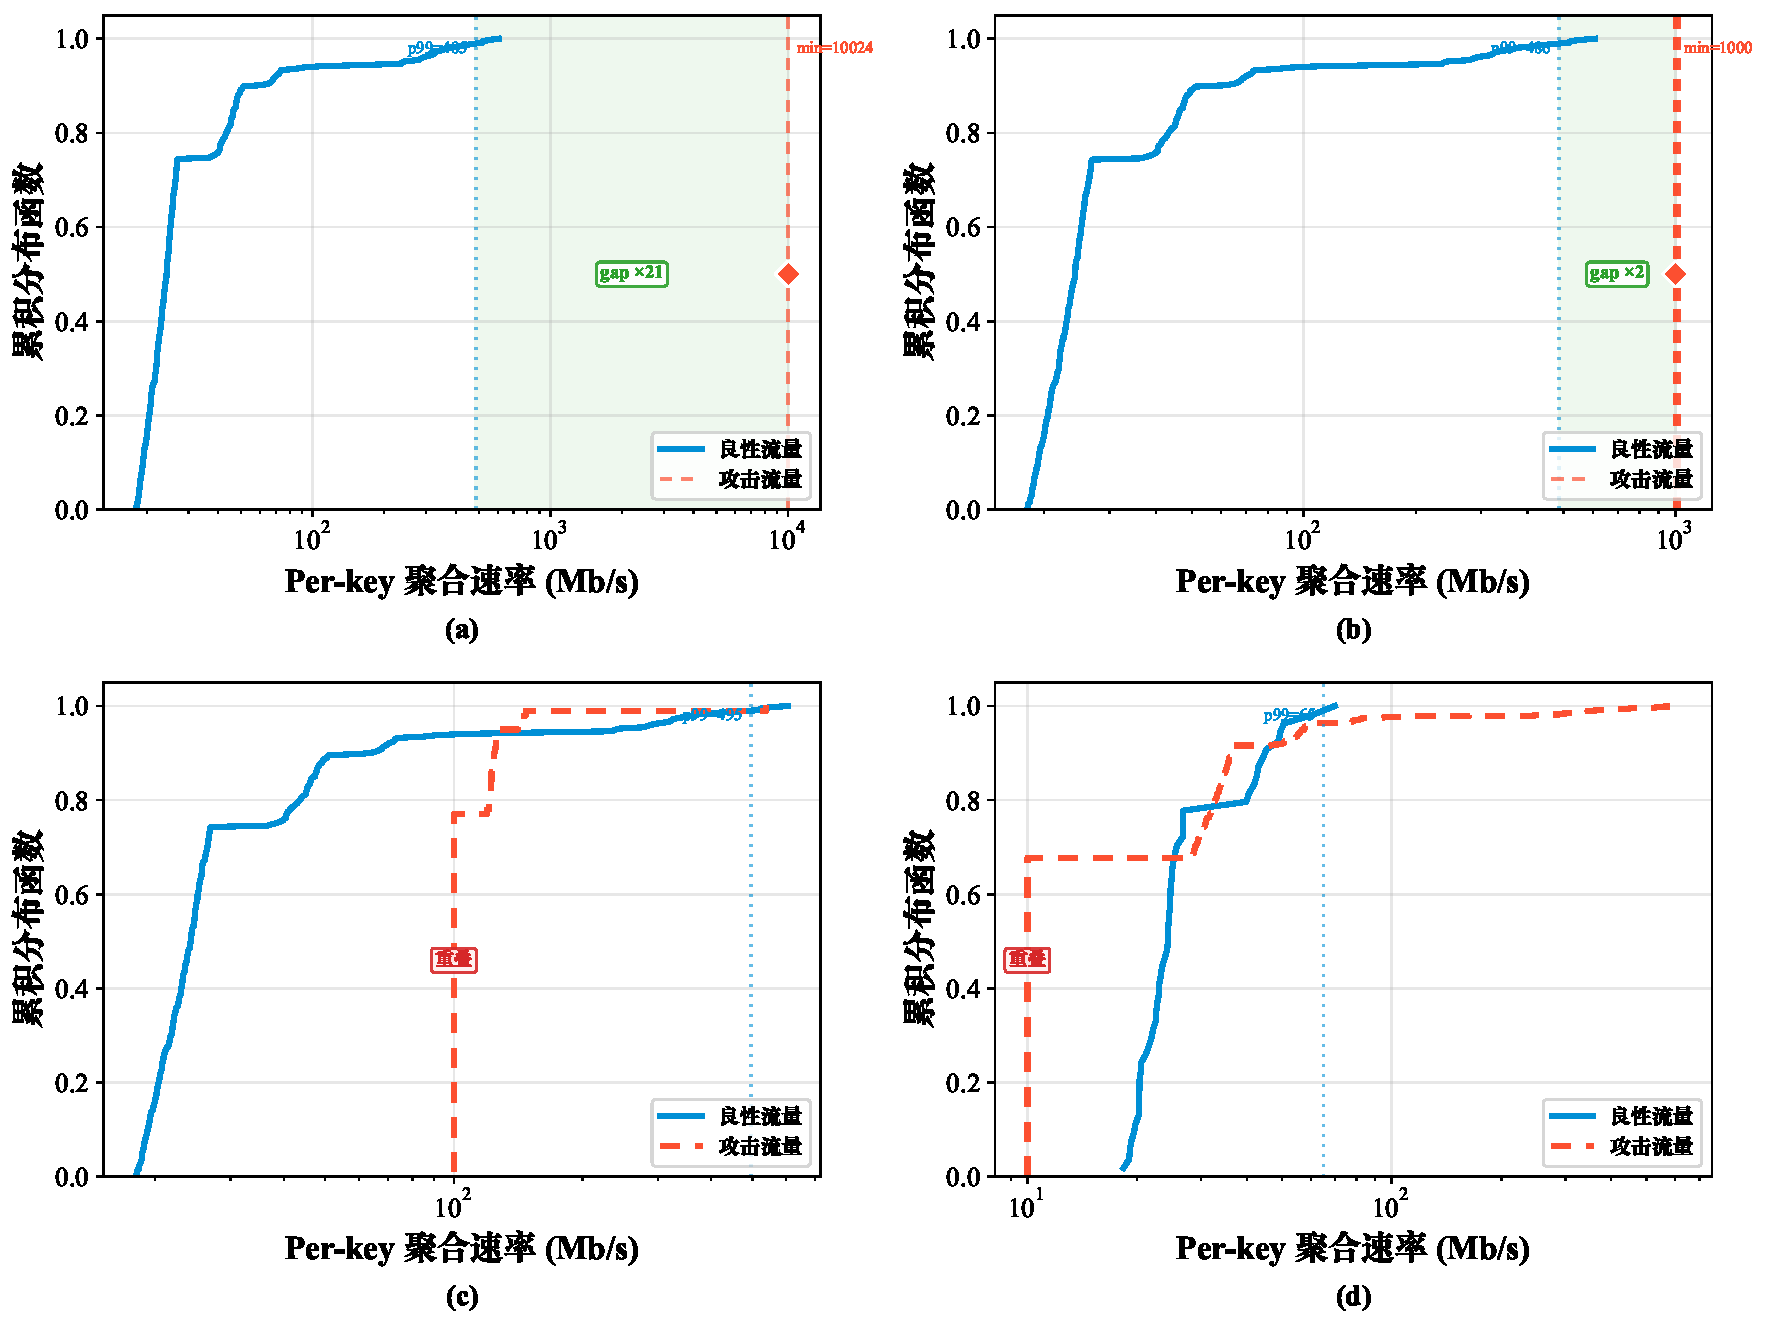
\includegraphics[width=0.92\linewidth]{figs/ch3/fig3_1_cdf.pdf}
  \caption{可分性随 decoy 数 $M$ 退化的 CDF 对比。四个子图分别对应 $M=1,10,100,1000$，蓝色实线为良性 key 聚合速率 CDF，红色虚线为攻击 key 聚合速率 CDF（$M\leq10$ 时因攻击 key 数量少，改用垂直线与散点标注）。绿色阴影区标注可分性间隙及倍数，红色 overlap 标注表示攻击与良性分布已交叉。}
  \label{fig:ch3_fig1_cdf}
\end{figure}

需要说明的是，图~\ref{fig:ch3_fig1_cdf} 中的可分性并非在任何条件下都成立。当攻击者采用更强的隐蔽策略时，速率特征可能退化并与良性长尾区间发生重叠。为明确方法的适用边界，并给出后续实验的退化路径，本章构造了三类典型设定：增大 bot 规模并降低单 bot 速率、将攻击流量分摊到更多 decoy 目的，以及采用脉冲式 on-off 策略使攻击 key 在窗口边界附近间歇出现。它们都满足 LFA 的基本约束，即总攻击注入量需要与目标链路剩余容量处于同一量级\citess{crossfire}：
\begin{equation}
\sum_{b\in\mathcal{B}} r_b \approx C_{e^\star}-U^{\text{benign}}_{e^\star},
\label{eq:lfa_budget}
\end{equation}
其中 $r_b$ 为 bot $b$ 的攻击发送速率，$U^{\text{benign}}_{e^\star}$ 为目标链路上良性占用带宽。式~(\ref{eq:lfa_budget}) 说明：如果希望将每个 key 的聚合速率压低到良性长尾附近，通常需要相应扩大可用 bot 数量或增大 decoy 分摊规模。如式~(\ref{eq:fi_lower}) 所示，这一过程中 fan-in/fan-out 至少一维往往会被放大，从而为多签名检测保留可利用的结构性痕迹。

\subsection{系统总览与数据流解释}
图~\ref{fig:ch3_fig5_arch} 展示了 MS-SatShield 的总体架构。系统由数据平面与星上代理（轻量控制平面）协同完成闭环：数据平面负责以线速维护基于 CMS 与候选缓存的一级候选生成摘要，并对活动候选执行轻量特征更新；星上代理以 epoch 为粒度拉取候选统计并计算多签名可疑度，将结果映射为队列优先级配置，再写回交换机用于下一轮调度。

\begin{figure}[!htb]
  \centering
  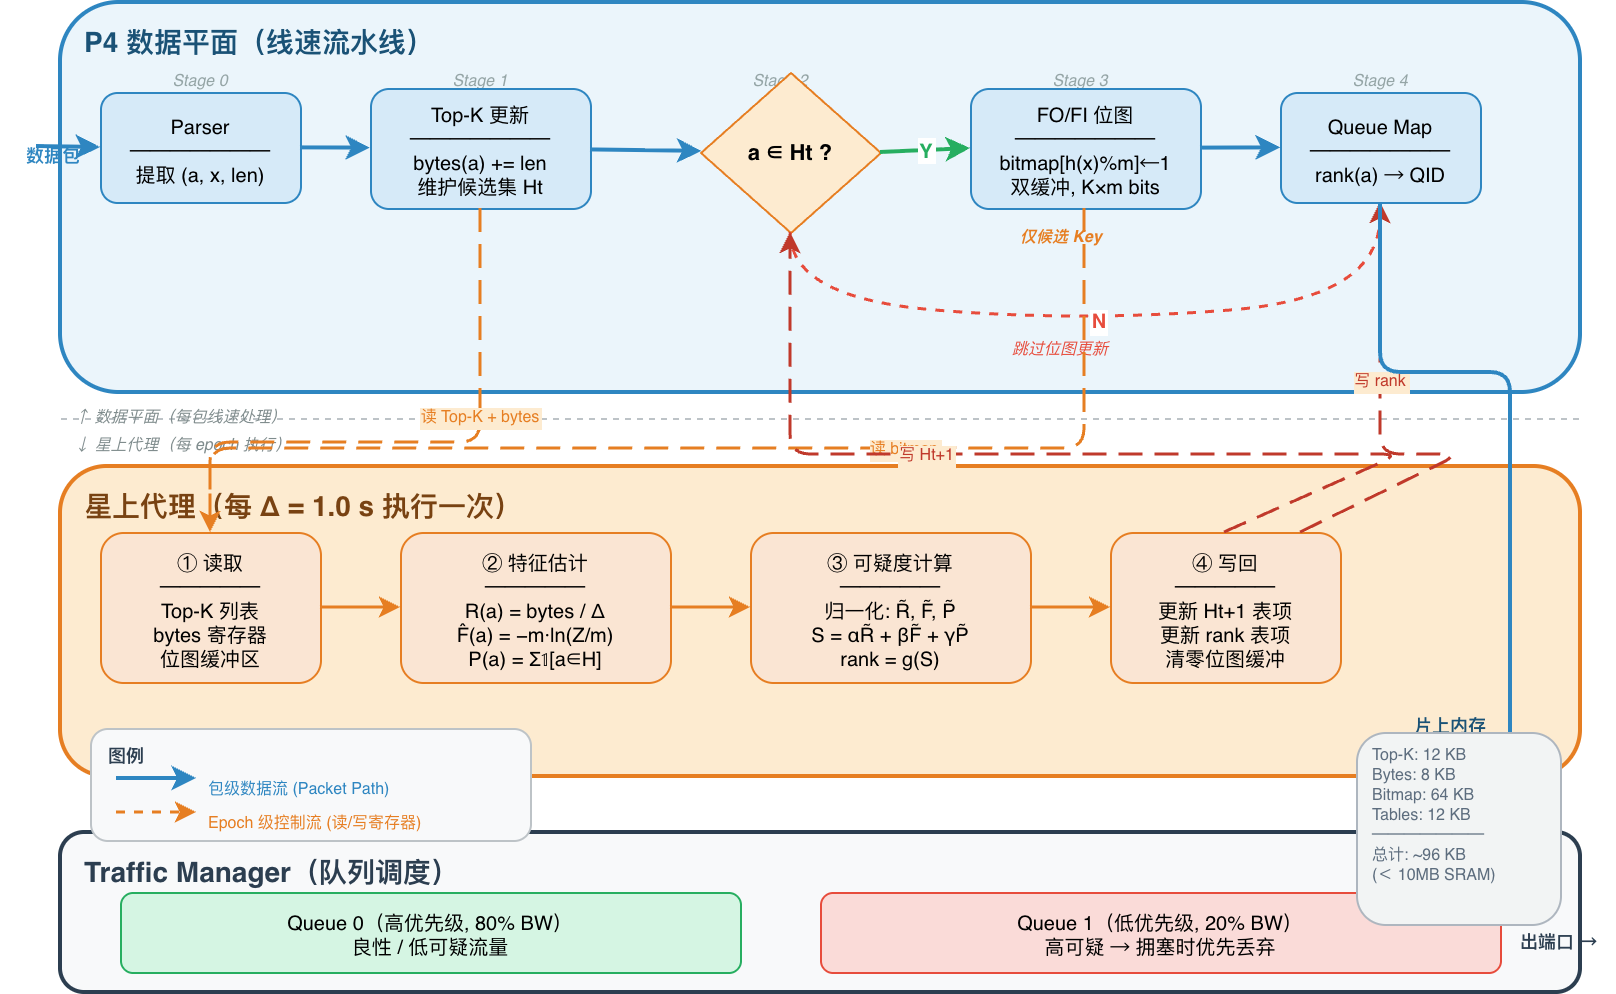
\includegraphics[width=0.96\linewidth]{figs/ch3/fig3-5_architecture.png}
  \caption{MS-SatShield 总体架构。数据平面逐包完成报文解析、CMS 与候选缓存更新、活动候选判定、FO/FI 位图更新与队列映射；星上 Agent 在每个 epoch 末读取候选摘要、字节统计与活动候选位图，估计速率、结构特征与持续性，生成下一轮活动候选配置与队列优先级映射，并写回交换机后由流量管理模块执行高/低优先级两队列调度。}
  \label{fig:ch3_fig5_arch}
\end{figure}

为了便于从处理流程理解图~\ref{fig:ch3_fig5_arch}，下面分别说明包级数据流与 epoch 级控制流。为避免时序歧义，本文保留 $\mathcal{H}_t$ 与 $\text{rank}_t(\cdot)$ 表示基于 epoch $t$ 统计结果导出的观测候选集与观测优先级，并记
\[
\mathcal{H}_t^{\mathrm{act}}=\mathcal{H}_{t-1},\qquad
\text{rank}_t^{\mathrm{act}}=\text{rank}_{t-1}.
\]
因此，在 epoch $t$ 的包处理中，交换机实际使用的是上一窗口导出的活动配置 $(\mathcal{H}_t^{\mathrm{act}},\text{rank}_t^{\mathrm{act}})$；而 epoch $t$ 结束后，代理根据当前窗口统计结果计算新的 $(\mathcal{H}_t,\text{rank}_t)$，并将其写回交换机，于 epoch $t+1$ 生效。

包级处理在交换机流水线中顺序发生。每个到达数据包 $p$ 在解析后得到地址 key $a$、对端 $x$ 与包长 $len$。系统先更新 CMS 计数矩阵，并依据当前估计频次刷新固定容量候选缓存；这一步对应一级候选生成，其目标是在固定内存内近似恢复当前窗口的重 key 集合及其显式 key 身份。对于驻留在候选缓存中的 key，数据平面同时维护候选级聚合字节计数寄存器 $\text{bytes}_t(a)$。随后系统判断该 key 是否命中活动候选集：若 $a\in\mathcal{H}_t^{\mathrm{act}}$，则进入 FO/FI 近似统计更新模块，将 $x$ 映射到位图索引并置位；若 $a\notin\mathcal{H}_t^{\mathrm{act}}$，则跳过 FO/FI 更新以节省状态访问。最后，系统依据当前已安装的队列优先级映射表 $\text{rank}_t^{\mathrm{act}}(\cdot)$ 选择队列并入队。这样安排后，CMS 更新与候选缓存刷新仍是所有数据包都必须执行的基础操作，而 FO/FI 更新只发生在活动候选集上，因此 distinct 统计的状态开销可以限制在 $O(K\cdot m)$。

epoch 级控制流由星上代理触发。代理按固定周期读取当前窗口的 CMS/候选缓存摘要与候选级字节计数，形成观测候选集合 $\mathcal{H}_t$；再读取活动候选 $\mathcal{H}_t^{\mathrm{act}}$ 对应的位图，用线性计数估计 $\widehat{F}_t(a)$，并更新持续性 $P_{t+1}(a)$；随后将 $R_t(a)$、$\widehat{F}_t(a)$、$P_t(a)$ 归一化并融合为可疑度 $S_t(a)$，再映射为下一轮活动优先级 $\text{rank}_{t+1}^{\mathrm{act}}(a)$ 并写回交换机。候选筛选、排序、归一化、对数或倒数等复杂运算都放在代理侧完成，数据平面只承担寄存器读写与简单算术，符合 PISA 流水线的可实现约束\citess{bosshart2013rmt}。

\subsection{基于 CMS 与候选缓存的一级候选生成}
与精确逐流状态不同，Count-Min Sketch（CMS）用固定大小的计数矩阵维护全局频率摘要，每包只需执行固定次数的哈希与计数更新，适合映射到 P4/PISA 流水线；但 CMS 本身不显式保存 key 身份，因此不能直接输出当前 top-$K$ key 列表。为同时兼顾\emph{全局频率估计}和\emph{显式 key 恢复}，MS-SatShield 在一级候选生成中采用 CMS 与固定容量候选缓存的组合：CMS 负责提供近似频率估计，候选缓存负责维护显式 key 集合及其候选级元数据。

具体地，设 CMS 由 $d$ 行、每行宽度为 $w$ 的计数矩阵 $\mathbf{S}_t\in\mathbb{N}^{d\times w}$ 构成，第 $i$ 行对应哈希函数 $h_i(\cdot)$。当包 $p$（长度为 $len$）携带 key $a$ 到达时，数据平面执行
\begin{equation}
\mathbf{S}_t[i,h_i(a)] \leftarrow \mathbf{S}_t[i,h_i(a)] + len,\qquad i=1,\ldots,d.
\label{eq:cms_update}
\end{equation}
随后，以各行对应计数器的最小值作为 key $a$ 在当前窗口的近似聚合字节估计：
\begin{equation}
\widehat{\text{bytes}}^{\mathrm{cms}}_t(a)=\min_{1\le i\le d}\mathbf{S}_t[i,h_i(a)],
\qquad
\widehat{R}^{\mathrm{cms}}_t(a)=\frac{\widehat{\text{bytes}}^{\mathrm{cms}}_t(a)}{\Delta}.
\label{eq:cms_query}
\end{equation}
式~(\ref{eq:cms_query}) 给出的是全局频率摘要，而非显式候选集合。为将其转化为后续多签名判决可直接使用的 key 列表，本文引入固定容量候选缓存
\begin{equation}
\mathcal{C}_t=\left\{(a,\text{bytes}_t(a),\text{meta}_t(a))\right\},\qquad |\mathcal{C}_t|\le K,
\label{eq:candidate_cache}
\end{equation}
其中每个缓存项保存显式 key 身份、候选级聚合字节计数 $\text{bytes}_t(a)$ 以及状态元数据 $\text{meta}_t(a)$（如有效位、时间戳或缓存索引等）。实现上，$\text{bytes}_t(a)$ 即由候选缓存项中的字节寄存器承载，并作为后续式~(\ref{eq:rate_def}) 中速率特征 $R_t(a)$ 的在网观测值。

候选缓存的更新规则如下：若到达 key $a$ 已存在于 $\mathcal{C}_t$，则直接刷新该项并累加 $\text{bytes}_t(a)$；若 $a\notin\mathcal{C}_t$ 且缓存未满，则插入新项；若缓存已满，则以 CMS 估计值作为替换依据。记
\begin{equation}
\theta_t=\min_{u\in\mathcal{C}_t}\widehat{\text{bytes}}^{\mathrm{cms}}_t(u),
\label{eq:cache_threshold}
\end{equation}
当 $\widehat{\text{bytes}}^{\mathrm{cms}}_t(a)>\theta_t$ 时，以 $a$ 替换当前缓存中估计最小的候选项。这里追求的是在固定容量 $K$ 下尽量恢复当前窗口中值得进入第二级判别的重 key 候选，而非在数据平面精确维护全局严格排序。因此，本文后续所称的 top-$K$ 候选，均指 CMS 与候选缓存联合恢复出的近似重流候选集合，而非精确的全局排序结果。

从资源角度看，一级候选生成器的状态预算可分解为
\begin{equation}
M_{\mathrm{CMS}}=\frac{dwb_{\mathrm{ctr}}}{8},\qquad
M_{\mathrm{cache}}=\frac{K\left(b_{\mathrm{key}}+b_{\mathrm{bytes}}+b_{\mathrm{meta}}\right)}{8},
\label{eq:stage1_budget}
\end{equation}
其中 $b_{\mathrm{ctr}}$ 为 CMS 计数器位宽，$b_{\mathrm{key}}$、$b_{\mathrm{bytes}}$ 与 $b_{\mathrm{meta}}$ 分别表示候选缓存中 key 标识、字节计数与元数据的位宽。在本文默认配置下，一级候选生成的开销通常为几十 KB，显著小于后续 FO/FI 位图区域的状态占用，因此整体资源占用仍主要由位图部分决定。


这一设计把两个任务拆开处理。CMS 在海量 key 空间中给出频率线索，候选缓存把少量需要继续观察的 key 显式保留下来。若只使用 CMS，系统虽然能估计频率上界，却无法直接枚举后续需要维护 FI/FO 的对象；若直接维护全量显式表，状态与查找代价又会随活跃 key 数量线性增长，超出星载环境可承受范围。一级候选生成器的目标因此不是精确求解 top-$K$，而是在固定状态预算下尽量恢复第二级判别所需的 key 身份。

从工程实现看，这一设计还给第二级特征统计划定了访问边界。由于 FO/FI 位图只对活动候选集维护，第二级的 bitmap、persist 与 queue mapping 状态都被限制在 $K$ 个对象之内。$K$ 因而不只是检测参数，也决定了整个数据面的内存上界与读写次数上界：一旦 $K$ 固定，distinct 近似统计、rank 表和辅助寄存器的规模也随之固定。这也是后续消融实验要专门讨论 $K$ 的原因。

\subsection{多签名可疑度建模与判决}
\label{subsec:ch3_score}
MS-SatShield 将一级候选生成与可疑判决分开处理：CMS 与候选缓存负责从海量 key 中筛选可疑候选集合 $\mathcal{H}_t$，多签名模型再在候选集合上区分攻击相关 key 与合法大流 key。为此，定义候选 key $a$ 的综合可疑度为
\begin{equation}
S_t(a)=\alpha \cdot \widetilde{R}_t(a) + \beta \cdot \widetilde{F}_t(a) + \gamma \cdot \widetilde{P}_t(a),
\label{eq:score_def}
\end{equation}
其中 $\alpha,\beta,\gamma$ 为权重，$\widetilde{(\cdot)}$ 为归一化后的特征值。权重的设计遵循如下原则：$\alpha$ 与 $\beta$ 为基础检测权重，满足 $\alpha+\beta=1$，使得仅由 rate 与 FI/FO 组成的基础分数 $S_t^{\text{base}}(a)=\alpha\widetilde{R}_t(a)+\beta\widetilde{F}_t(a)\in[0,1]$；$\gamma$ 为持续性的加性奖励权重（additive bonus），独立于基础权重之外，其作用是为反复出现的可疑 key 提供额外加分。当 $\gamma=0$ 时退化为双签名方案 S1；当 $\gamma>0$ 时，$S_t(a)$ 的值域扩展为 $[0,1+\gamma]$，但由于 $\gamma$ 较小（本文取 $\gamma=0.2$），阈值 $\tau=0.5$ 的判决语义不受实质影响——$\tau$ 仍位于基础分数值域 $[0,1]$ 的中点，持续性仅为已超过 $\tau$ 的 key 提供额外置信度提升。本文默认取 $\alpha=\beta=0.5$, $\gamma=0.2$。

归一化的目的在于使不同量纲、不同尺度的特征在同一分数空间可加。本文采用分位数归一化：以良性流量历史统计得到的分位点作为尺度基准，例如
\begin{equation}
\widetilde{R}_t(a)=\min\left(1,\frac{R_t(a)}{Q_{0.99}(R^{\text{benign}})}\right),\quad
\widetilde{F}_t(a)=\min\left(1,\frac{\widehat{F}_t(a)}{Q_{0.99}(F^{\text{benign}})}\right),
\label{eq:norm_def}
\end{equation}
其中 $Q_{0.99}(\cdot)$ 表示 $0.99$ 分位点。$Q_{0.99}$ 可通过离线分析良性 trace 获得并作为配置参数写入代理；在线场景下亦可采用滑动窗口分位数估计，但需确保窗口长度覆盖多个 epoch 以避免被攻击流量污染。持续性 $\widetilde{P}_t(a)$ 可直接按窗口长度 $k_p$ 归一化为 $\widetilde{P}_t(a)=P_t(a)/k_p$。

在给出检测判决之后，系统还需要将分数空间映射到队列优先级空间。结合当前实验与实现口径，本文采用高/低优先级两队列体系，并定义下一轮活动优先级
\begin{equation}
\text{rank}_{t+1}^{\mathrm{act}}(a)=g(S_t(a))\in\{0,1\},
\label{eq:rank_map}
\end{equation}
其中较小的 $\text{rank}$ 表示较高优先级。本文采用二值阈值映射：
\begin{equation}
g(S_t(a))=\begin{cases}
0, & \text{if } S_t(a)<\tau,\\
1, & \text{if } S_t(a)\geq\tau.
\end{cases}
\label{eq:g_def}
\end{equation}
其中 $S_{\max}=1+\gamma$ 为可疑度的理论上界（$\gamma=0$ 时 $S_{\max}=1$），$\tau$ 为检测阈值。当 $S_t(a)<\tau$ 时，key 被分配到高优先级队列并保留高优先级带宽份额；当 $S_t(a)\geq\tau$ 时，key 被分配到低优先级队列，在拥塞时优先承受丢弃。若将来扩展到多级优先级队列，可在此基础上将 $g(\cdot)$ 泛化为多段映射；但本文实验不展开该扩展。

\subsection{FO/FI 在网近似统计结构}
在网环境中对每个 key 精确维护式~(\ref{eq:fan_def}) 的 distinct 计数会导致状态空间与更新开销不可接受。为保持可实现性，MS-SatShield 仅对候选集合 $\mathcal{H}_t$ 维护 FO/FI 的近似统计结构。本章以位图（bitmap）作为主线实现\citess{whang1990linear}，原因在于其数据平面更新简单（置位操作）且内存预算可直接计算。

对每个候选 key $a$，分配一个长度为 $m$ 的位图 $\text{bitmap}_t(a)\in\{0,1\}^m$。每当观察到关系对 $(a,x)$，计算
\begin{equation}
i=h(x)\bmod m,\qquad \text{bitmap}_t(a)[i]\leftarrow 1,
\label{eq:bitmap_update}
\end{equation}
其中 $h(\cdot)$ 为哈希函数。epoch 末在星上代理侧读取位图，令 $Z$ 为位图中 0 的个数，则可用线性计数\citess{whang1990linear}估计 distinct 基数：
\begin{equation}
\widehat{F}_t(a) = -m\cdot \ln\left(\frac{Z}{m}\right).
\label{eq:linear_count}
\end{equation}
式~(\ref{eq:linear_count}) 的计算包含对数运算，因此由代理完成，数据平面只负责置位更新。为避免每个 epoch 全量清零位图带来额外开销，同时减少攻击者利用窗口边界的空间，本文采用双缓冲位图：奇偶 epoch 交替写入不同缓冲区，读取后由代理对上一缓冲区批量清零，从而避免数据平面执行大规模清理操作。具体而言，代理在每个 epoch 末通过控制平面 API 翻转一个单比特寄存器 \texttt{epoch\_parity}，数据平面据此选择写入的位图实例，无需流水线自行判断窗口切换。

若按部署口径同时为 FI 与 FO 两个视角各维护一组双缓冲位图，则位图状态预算为
\begin{equation}
M_{\text{bitmap}}^{\text{deploy}} = \frac{4Km}{8}\ \text{Bytes},
\label{eq:bitmap_budget}
\end{equation}
其中系数 $4$ 分别对应 FI/FO 两个视角与奇偶双缓冲两组实例。在此基础上，总数据面状态预算可近似写为
\begin{equation}
M_{\text{total}} \approx M_{\mathrm{CMS}} + M_{\mathrm{cache}} + M_{\text{bytes}} + M_{\text{bitmap}}^{\text{deploy}} + M_{\text{rank}} + M_{\text{aux}}.
\label{eq:total_budget}
\end{equation}
需要说明的是，位图结构的误差会随着真实基数接近或超过 $m$ 而快速增大，即出现饱和。但在本章场景中，FO/FI 主要用于区分正常情况下较小的 FO/FI 与攻击导致的显著放大，并不要求精确估计超大规模基数。因此，在有限内存下位图依然可以作为有效的判别签名。若需要覆盖更大的 FO/FI 范围，可采用 HLL-lite 结构提高抗饱和能力；本文聚焦 bitmap 主线实现，暂不展开对比实验。


选择位图加线性计数，是面向星载实现条件做出的取舍。对本文来说，FI/FO 只要能把正常情况下较小的扇入/扇出与攻击造成的明显放大区分开即可，无需在极大基数范围内追求最优无偏估计。这样一来，数据面只需完成哈希和置位，对数运算留给 agent 侧处理，逐包快路径仍保持常数次寄存器访问。若直接在数据面实现 HLL 或更复杂的 distinct 估计逻辑，寄存器读写与比较操作都会增加，也更难适配星载 PISA 的约束。

双缓冲不只是为了方便清零。它把窗口切换时的大规模状态重置从逐包快路径中剥离出来，避免攻击者利用窗口边界制造瞬时状态不一致；同时，奇偶缓冲交替写入保证当前 epoch 的统计始终对应一块干净位图，而上一块位图可以在 agent 侧按批次读取和清理。这种时序安排与前文定义的 epoch 级控制流保持一致。

\subsection{多签名在网检测与队列调度流程}
算法~\ref{alg:ms_satshield} 给出了 MS-SatShield 的整体流程。该流程与图~\ref{fig:ch3_fig5_arch} 一一对应，并明确区分了数据平面逐包处理与星上代理逐 epoch 更新。

\begin{algorithm}[t]
\caption{\textsc{MS-SatShield} 多签名在网检测与队列调度流程}
\label{alg:ms_satshield}
\Input{(1) 当前到达数据包 $p=\langle a,x,len\rangle$；\newline
(2) 当前窗口数据面状态：CMS 计数矩阵 $\mathbf{S}_t$、候选缓存 $\mathcal{C}_t$、候选级字节计数 $\text{bytes}_t(\cdot)$、活动候选集 $\mathcal{H}_t^{\mathrm{act}}$、位图 $\text{bitmap}_t(\cdot)$；\newline
(3) 控制面状态与参数：持续性 $P_t(\cdot)$、epoch 长度 $\Delta$、位图长度 $m$、评分权重 $\alpha,\beta,\gamma$。}
\Output{当前包的队列优先级决策，以及下一轮活动候选配置 $(\mathcal{H}_{t+1}^{\mathrm{act}}, \text{rank}_{t+1}^{\mathrm{act}}(\cdot))$。}

\tcc{步骤 1：数据平面逐包更新一级候选与候选级统计}
解析得到地址 key $a$（源地址或目的地址）、对端地址 $x$（目的地址或源地址）以及包长 $len$\;
更新 CMS 计数矩阵（以 $(a,len)$ 更新 $d$ 个 counter）并按当前估计值刷新候选缓存 $\mathcal{C}_t$\;
\If{$a \in \mathcal{C}_t$}{
    累加候选级字节计数 $\text{bytes}_t(a)\leftarrow \text{bytes}_t(a)+len$\;
}
\BlankLine
\tcc{步骤 2：对活动候选更新 FO/FI 位图并完成当前包入队}
\If{$a \in \mathcal{H}_t^{\mathrm{act}}$}{
    计算 $i=h(x)\bmod m$，并置位 $\text{bitmap}_t(a)[i]\leftarrow 1$\;
}
根据当前映射表 $\text{rank}_t^{\mathrm{act}}(\cdot)$ 确定队列优先级并入队\;

\BlankLine
\tcc{步骤 3：星上代理在 epoch 末生成下一轮活动配置}
从数据平面读出当前窗口的 CMS/候选缓存摘要与 $\text{bytes}_t(\cdot)$，形成观测候选集合 $\mathcal{H}_{t}$\;
\If{$\gamma>0$}{
  将 $\{a \mid P_t(a)\geq 2,\; a\notin\mathcal{H}_{t}\}$ 合并到评分候选集 $\mathcal{H}_{t}$（持续性扩展）\;
}
读取 $\mathcal{H}_t^{\mathrm{act}}$ 的位图并由式~(\ref{eq:linear_count}) 估计 $\widehat{F}_t(\cdot)$，更新持续性 $P_{t+1}(\cdot)$\;
由式~(\ref{eq:rate_def})--(\ref{eq:score_def}) 计算多签名可疑度 $S_t(\cdot)$ 并由式~(\ref{eq:g_def}) 映射为下一轮活动优先级 $\text{rank}_{t+1}^{\mathrm{act}}(\cdot)$\;
令 $\mathcal{H}_{t+1}^{\mathrm{act}}\leftarrow\mathcal{H}_{t}$，并将 $\mathcal{H}_{t+1}^{\mathrm{act}}$ 与 $\text{rank}_{t+1}^{\mathrm{act}}(\cdot)$ 写回交换机表项，使其在 epoch $t+1$ 生效\;
切换/清理位图缓冲区以开始下一 epoch\;
\textbf{return} 当前包的队列优先级决策，以及下一轮活动候选配置 $(\mathcal{H}_{t+1}^{\mathrm{act}}, \text{rank}_{t+1}^{\mathrm{act}}(\cdot))$\;
\end{algorithm}


\subsubsection*{单个epoch的运行示例}
下面给出一个以目的地址为 key 的单窗口示例。设某 decoy 目的地址 $a_d$ 在 epoch $t$ 内同时接收来自大量 bots 的低速访问。对经过受害卫星的数据包，数据平面先将每个匹配 $a_d$ 的数据包写入 CMS，并不断抬升其在候选缓存中的近似频次；当 $a_d$ 稳定驻留在候选缓存后，候选级字节计数 $\text{bytes}_t(a_d)$ 持续累加。由于当前实验默认以目的地址为 key，数据平面对每个不同源地址 $x$ 仅做一次位图置位，因此窗口结束时会形成较大的 $\widehat{F}_t(a_d)$。如果 $a_d$ 在前若干窗口中也多次进入候选集，则其持续性 $P_t(a_d)$ 也会较高。epoch 结束后，agent 读取这些统计量并计算 $S_t(a_d)$；当其超过阈值 $\tau$ 时，$a_d$ 会在 epoch $t+1$ 被映射到低优先级队列，后续所有发往 $a_d$ 的流量在拥塞时都会优先承受丢弃。相对地，正常热门目的地址虽然可能具有较高的 $R_t(a)$，但若其 FI 明显低于攻击类 decoy，或者只在短时间内进入候选集，则综合得分仍可能低于阈值，从而保留在高优先级队列。这个例子表明，MS-SatShield 的效果来自频率筛选、结构判别、历史记忆和队列执行之间的配合，而不是某个单独特征。

\section{实验设置与结果分析}
\subsection{实验平台与基线方案}
为验证 MS-SatShield 的检测与缓解效果，本文搭建了由 LEO 攻击仿真、P4/PISA 约束下的数据面原型设计和流量重放评估组成的实验框架。LEO 层面采用与 ICARUS/SatShield 一致的仿真参数与星座模型（基于 Hypatia\citess{hypatia} 仿真框架），以保证攻击与背景流量分布具有可对齐的现实依据\citess{icarus,satshield}；数据平面层面按 P4\citess{bosshart2014p4} 的可编程流水线约束实现 CMS 频率估计、固定容量候选缓存更新、候选位图更新与两队列优先级映射；星上代理在每个 epoch 周期性读取寄存器并下发队列优先级映射。
\subsubsection*{实验执行流程}
每轮实验按四个顺序步骤执行。在给定 epoch 长度 $\Delta$ 与当前拓扑快照 $G_\tau$ 的条件下，仿真器先生成该窗口内的链路状态、最短路径与目标链路位置，并据此确定背景流与攻击流的转发路径。随后，流量重放模块将良性 trace 映射为地面终端对之间的业务请求，再叠加满足式~(\ref{eq:lfa_budget})的攻击流，形成带标签的逐包输入序列。接着，输入序列按时间顺序送入在网处理程序，由数据平面逐包执行 CMS 更新、候选缓存刷新、活动候选位图置位与队列映射，同时由星上代理在 epoch 末读取寄存器摘要并生成下一轮 rank 配置。最后，离线评估脚本依据攻击生成器输出的标签文件，对 detector 级和 identifier 级结果分别计算 Precision、Recall、F1，并汇总反应时间与良性吞吐等缓解指标。

这样拆分之后，观测、判决和生效三个时序阶段被明确分开。对任意一个 epoch，数据平面实际执行的是上一窗口导出的活动配置 $(\mathcal{H}_t^{\mathrm{act}},\text{rank}_t^{\mathrm{act}})$，当前窗口只负责生成下一轮配置。这一时序与前文的双缓冲位图和 epoch 级控制流定义保持一致，也意味着后文讨论的 reaction time 表示攻击出现、当前窗口统计完成以及下一窗口缓解生效在内的闭环生效时间，而不是单次表项写入延迟。

基线对比方案主要包括：
\begin{enumerate}
\item SatShield（rate-only，记为 S0）：仅使用归一化聚合速率 $\widetilde{R}_t(a)$ 作为可疑度（即 $\alpha=1,\beta=\gamma=0$），通过阈值 $\tau=0.5$ 进行二元判决。该基线是 SatShield 原文\citess{satshield} 在本文框架内的等效实现，保留了其一级候选生成与速率阈值判决的基本逻辑；
\item MS-SatShield（rate + FO/FI，记为 S1）：在候选集合上加入 $\widehat{F}_t(a)$，取 $\alpha=\beta=0.5,\gamma=0$；
\item MS-SatShield（rate + FO/FI + persist，记为 S2）：进一步加入持续性 $P_t(a)$，取 $\alpha=\beta=0.5,\gamma=0.2$，用于对抗脉冲式攻击与候选抖动。
\end{enumerate}

\subsubsection*{基线可比性与公平性说明}
本章三组基线只在第二级判别特征上存在差异，其余实验条件保持一致：采用相同的拓扑与路由快照、相同的背景与攻击输入、相同的一级候选生成器（CMS + 候选缓存）、相同的 key 视角（默认目的地址）、相同的二值队列结构，以及相同的检测阈值 $\tau=0.5$。因此，S0、S1、S2 的比较实际发生在仅速率、速率加结构、速率加结构再加历史三种设置之间，用来考察每个新增签名带来的边际收益。这样设置后，一旦结果发生变化，就可以更直接地归因到新增特征本身，而不是候选生成、队列策略或实现细节的差异。

三种方案均使用相同阈值 $\tau=0.5$。由于 S0 与 S1 的可疑度值域均为 $[0,1]$，$\tau=0.5$ 的判决语义一致；S2 的 $\gamma=0.2$ 是加性奖励（见 \S\ref{subsec:ch3_score}），不会改变基础判决逻辑，因此共用 $\tau$ 仍然公平。这样的对比也与后续消融实验的三个层级保持一致。

% [INS-ICARUS-09]
此外，ICARUS 在同一星座配置下采用了空载网络、GDP gravity 与人口 gravity 三类背景流量场景，并通过地理网格离散化评估区域级连通性影响。本文不复现其全量攻击优化流程，而是沿用 SatShield 的带标签流量回放与在网检测、缓解这一实验主线，用来回答单节点检测器在退化策略下的区分能力问题。两类实验关注的重点不同：ICARUS 更强调攻击可达性与代价-可检测性权衡，本文更强调在网检测与缓解精度。为避免混淆，结果对比仅在共享参数与共享指标语义下进行\citess{icarus,satshield}。

\subsection{数据集、流量生成与参数设置}
良性背景流量采用 CAIDA 匿名 trace 进行重放，并依据人口（Pop）分布模型映射为城市对之间的通信需求；同时保证背景流量不会使任意链路长期超过 $90\%$ 利用率，以避免“未攻击已拥塞”的非预期干扰\citess{satshield}。攻击流量由 LFA 生成器构造：在每个攻击实验中随机选取城市对作为受害通信对，选择目标链路 $e^\star$ 并生成满足式~(\ref{eq:lfa_budget}) 的攻击注入速率。表~\ref{tab:ch3_params} 总结了主要的网络与终端参数。

% [INS-ICARUS-10]
需要说明的是，ICARUS 为了分离攻击最低资源门槛与背景噪声干扰，常采用无良性流量的保守场景作为上界评估；本文则采用含良性背景的重放场景，更接近部署侧的观测条件。两种设定并不矛盾：前者用于估计最坏情况下的攻击可行性，后者用于检验检测器在真实流量长尾存在时的稳健性。本文报告的检测收益不直接外推为最低攻击成本结论，而是作为给定背景流量下的防御性能证据\citess{icarus,satshield}。


\subsubsection*{良性背景流量的构造与映射}
选择 CAIDA 匿名互联网 trace 作为良性背景，主要基于两点。该数据集包含真实互联网主干链路中的长尾分布、突发性与热门目的地效应，比人工合成的 Poisson/CBR 流更容易暴露 rate-only 检测器在合法大流与攻击聚合之间的区分困难；同时，SatShield 已在同类 LEO-LFA 评估中采用相近的数据来源与映射思路，便于与既有结果建立可对齐的比较口径。本文并不依赖 CAIDA 在绝对业务占比上的完全真实性，而是利用其提供的真实长尾结构，检验检测器在存在正常重流时是否仍具有区分能力。

具体构造时，原始 trace 先按链路容量尺度进行比例缩放，使重放后的背景负载与 20~Gb/s 量级的 ISL 场景相匹配；再依据人口加权的城市对模型，将 trace 中的通信需求映射为 LEO 地面终端之间的源宿请求。这样的两阶段映射可以减少直接把互联网 trace 原样投射到星座链路所带来的失真：前一阶段保证负载量级与星座容量约束一致，后一阶段将业务空间分布与地理人口分布联系起来，使热点城市之间更容易形成较高的正常通信强度。为避免背景流量本身持续压满链路，本文进一步约束任意链路的长期良性利用率不超过 $90\%$，从而保证后续观测到的拥塞主要由攻击注入触发，而不是由背景配置不当造成。

\subsubsection*{攻击流生成与Ground Truth定义}
攻击流量的生成遵循 LFA 的基本构造逻辑：先在当前快照上选定目标链路 $e^\star$，再从其上游可达区域选择 bots、从下游可达区域选择 decoys，使 bot 到 decoy 的转发路径在统计意义上尽可能汇聚到 $e^\star$ 上。为保证不同退化设定之间具有可比性，本文在比较 $M$ 或 on/off 节律时，尽量保持总攻击注入量 $A$ 处于同一量级，只改变每个目的地址承载的攻击聚合速率，以及这些 key 在相邻 epoch 中是否连续出现。这样可以更明确地将实验结论归因于特征退化方式本身，而不是攻击总强度的变化。

由于后续实验默认以目的地址作为 key，ground truth 也按目的地址口径定义：凡是在当前实验配置下被攻击生成器选为 decoy，且其攻击路径穿越目标链路 $e^\star$ 的目的地址，均记为正类集合 $F$；未被攻击生成器选中的其他目的地址记为负类。这里强调标签与聚合粒度的一致性。检测器观察的是目的地址级聚合流量，而不是单条五元组流，因此标签也必须落在目的地址层级，不能混用包级或流级标签。若某一目的地址同时承载背景流量与攻击流量，只要其在观测窗口内存在攻击贡献，仍将其视为攻击相关 key。该定义与式~(\ref{eq:f1_def})的集合口径保持一致，也使后续 Precision/Recall/F1 反映的是是否识别出攻击相关聚合对象，而不是某条具体微流。

\begin{table}[t]
\centering
\caption{实验主要参数设置（与 SatShield/ICARUS 对齐）}
\label{tab:ch3_params}
\begin{tabular}{l l}
\hline
参数 & 取值 \\
\hline
星座拓扑 & Starlink Shell 1（1584 颗卫星） \\
ISL 容量 $C_e$ & 20 Gb/s \\
单终端上行/下行峰值 & 64 Mb/s / 384 Mb/s \\
单星最大服务终端数 & 2080 \\
背景流量来源 & CAIDA trace 重放并按 Pop 模型映射 \\
epoch 长度 $\Delta$ & 1.0~s \\
候选规模 $K$ & $\mathrm{clip}(0.3\cdot N_{\text{keys}},\;50,\;1000)$（自适应）\footnote{$N_{\text{keys}}$ 为上一 epoch 中一级候选生成器（CMS + 候选缓存）报告的活动 key 估计数量。} \\
位图长度 $m$ & 256~bits \\
持续窗口 $k_p$ & 5~epochs \\
可疑度阈值 $\tau$ & 0.5 \\
活动队列数 $Q$ & 2（高/低优先级） \\
高优先级带宽比 & 0.8（80\% 带宽保留给良性/低可疑流量）\\
\hline
\end{tabular}
\end{table}

为了展示速率特征退化后多签名如何恢复检测能力，本文在保持总攻击注入量 $A$ 基本不变的前提下，构造了多 decoy 分摊的退化设定。表~\ref{tab:ch3_deg_decoy} 给出了这一设定的参数组。表中包含 $M=1$ 的下界情形，它仅作为对照，用来展示当每个目的聚合速率极大时，rate-only 可以稳定工作；随着 $M$ 增大，单 decoy 的聚合速率约为 $A/M$，并逐步逼近正常业务的长尾区间，从而使 rate-only 的候选质量下降，也引出 FI/FO 的必要性。

\begin{table}[t]
\centering
\caption{退化设定：多 decoy 分摊（降低按目的聚合速率，放大 fan-in/fan-out）}
\label{tab:ch3_deg_decoy}
\begin{tabular}{c r r r r r}
\hline
组别 & $|\mathcal{B}|$ & $r$ (Mb/s) & $A$ (Gb/s) & $M$ & 约单 decoy 聚合速率 $A/M$ \\
\hline
B1 & 2000 & 5 & 10 & 1    & 10 Gb/s \\
B2 & 2000 & 5 & 10 & 10   & 1 Gb/s \\
B3 & 2000 & 5 & 10 & 100  & 100 Mb/s \\
B4 & 2000 & 5 & 10 & 1000 & 10 Mb/s \\
\hline
\end{tabular}
\end{table}

\subsection{评价指标与绘制方式}
检测侧采用 Precision、Recall、F1 作为主要指标。令真实攻击相关 key 集合为 $F$，算法输出集合为 $\widehat{F}$，则
\begin{equation}
\text{Precision}=\frac{|F\cap \widehat{F}|}{|\widehat{F}|},\qquad
\text{Recall}=\frac{|F\cap \widehat{F}|}{|F|},\qquad
\text{F1}=\frac{2\cdot \text{Precision}\cdot \text{Recall}}{\text{Precision}+\text{Recall}}.
\label{eq:f1_def}
\end{equation}
其中 $F$ 的定义需与攻击生成器一致：若以源地址为 key，则 $F$ 定义为 bot 源地址集合；若以目的地址为 key，则 $F$ 定义为 decoy 目的地址集合。缓解侧采用反应时间（reaction time）与良性吞吐下降（throughput drop）等指标，与 SatShield 的定义保持一致：reaction time 表示从观测到首个攻击包到系统开始生效缓解的时间间隔；throughput drop 表示攻击发生前后良性吞吐的下降比例\citess{satshield}。


\subsubsection*{指标统计口径与解释边界}
本章同时报告 detector 级指标与最终识别级指标，因为 MS-SatShield 具有清晰的两级结构：第一级回答攻击相关 key 是否进入候选集，第二级回答进入候选后能否被正确赋予较低优先级。若只报告最终 F1，就无法区分性能下降究竟来自候选覆盖不足，还是来自候选内判别失败。将两者拆开后，便可以像图~\ref{fig:ch3_fig2_f1}(a) 那样，更准确地定位 rate-only 方案的失效位置。

除时域曲线外，本文对吞吐与反应时间的统计都采用攻击期口径，而不是全时段口径。具体来说，良性吞吐比例按攻击持续阶段的 epoch 级结果计算并求平均，以免 warmup 与攻击结束后的恢复段稀释缓解差异；reaction time 则以首个攻击包进入系统为起点，以首批低优先级缓解规则在数据面实际生效为终点，因此反映的是包含一个 epoch 观测与配置延迟在内的闭环响应时间，而不是单次表项写入延迟。对于 on-off 场景，文中另外给出时域曲线，用于展示切换边界处的抖动与恢复过程。

图~\ref{fig:ch3_fig2_f1} 的绘制流程如下：对每组实验参数，先利用仿真器与流量重放器生成带标签的包序列；再将包序列输入在网处理程序，完成逐包处理与逐 epoch 统计；最后在离线评估脚本中按式~(\ref{eq:f1_def}) 计算 Precision、Recall 和 F1 并绘制曲线。为与 SatShield 的复现逻辑对齐，本文同时给出一级候选捕获准确性（对应 detector）与攻击相关 key 识别准确性（对应多签名判决）两类 F1 结果，从而将候选生成质量与候选内判别能力分开分析，避免混淆误差来源。

\begin{figure}[!htb]
  \centering
  \subfloat[rate-only 检测器各指标随 $M$ 变化]{%
    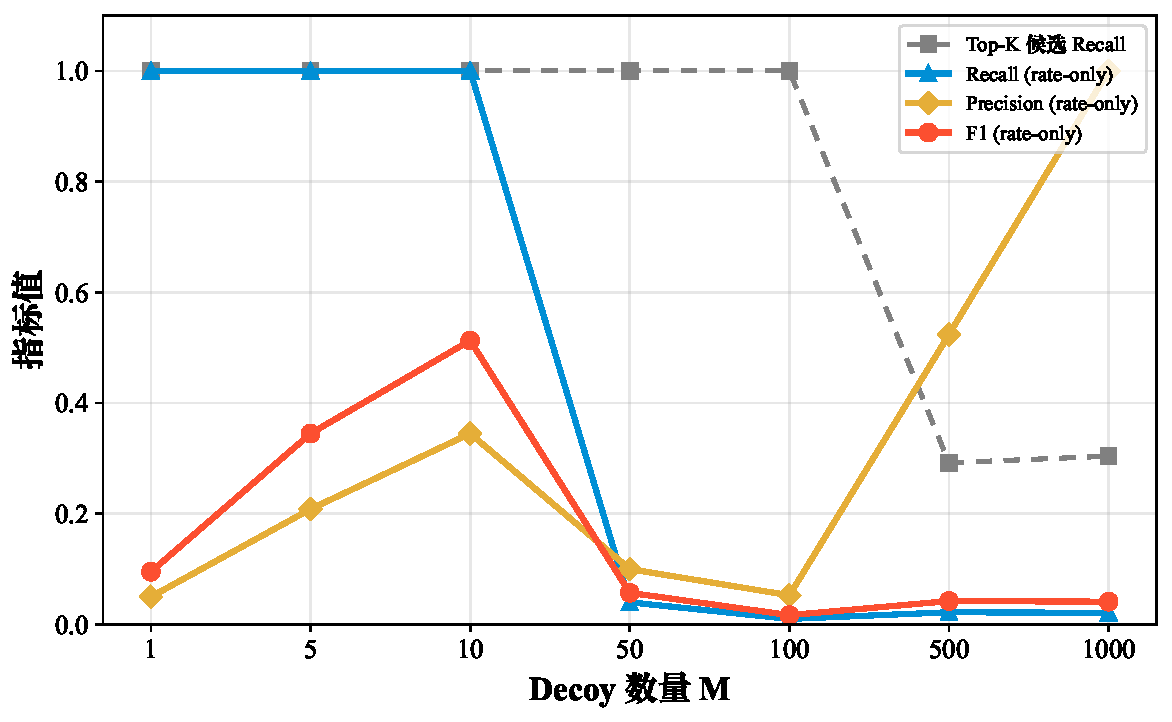
\includegraphics[width=0.48\linewidth]{figs/ch3/fig3_2a_topk_f1.pdf}%
  }%
  \hfill
  \subfloat[S0(rate-only) vs S1(+FO/FI) 的 F1 对比]{%
    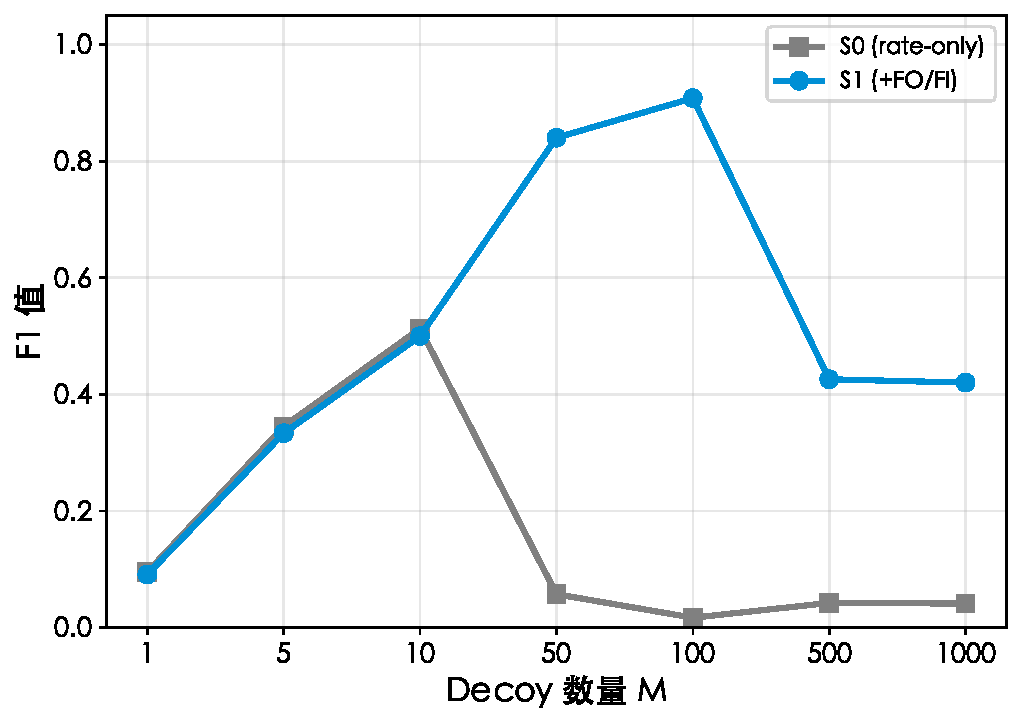
\includegraphics[width=0.48\linewidth]{figs/ch3/fig3_2b_degrade_f1.pdf}%
  }
  \caption{退化攻击下的检测性能。(a) 仅靠聚合速率（rate-only）的一级候选 Recall、阈值判决 Recall/Precision/F1 随 decoy 数 $M$ 的变化；(b) rate-only (S0) 与引入 FO/FI 后 (S1) 的 F1 对比，展示 FO/FI 特征在静态退化场景下的作用。ground truth 以 decoy 目的地址为 key。}
  \label{fig:ch3_fig2_f1}
\end{figure}

\subsection{结果分析：退化证据链与多签名收益}

\noindent\textbf{（1）可分性分析与一级候选诊断}\quad
图~\ref{fig:ch3_fig1_cdf} 从分布层面验证了速率可分性随 $M$ 退化的完整过程。$M=1$ 时，良性 $p_{99}\approx485$~Mb/s 与攻击聚合速率 $10{,}024$~Mb/s 之间存在约 $21$ 倍间隙，一级候选生成器可轻松捕获攻击 key。随着 $M$ 增大到 $100$，攻击 key 的 per-key 速率降至 $100$~Mb/s，已完全融入良性长尾区间，速率特征失去区分力。

图~\ref{fig:ch3_fig2_f1}(a) 从检测管线角度进一步诊断了 rate-only 方案的失效模式。该图同时给出一级候选 Recall、阈值判决 Recall、Precision 与 F1 四条曲线。当 $M\leq100$ 时一级候选 Recall 保持 $1.0$，说明候选生成模块在中等退化下仍具备完整的攻击 key 捕获能力；然而阈值判决 Recall 在 $M=50$ 时骤降至 $0.04$，F1 全程不超过 $0.52$，表明 rate-only 方案的瓶颈在于判决阈值无法区分攻击 key 与良性重流 key。当 $M\geq500$ 时，一级候选 Recall 本身亦降至约 $0.3$，意味着大量攻击 key 的聚合速率已低于良性 key 而被候选生成器排除。需要说明的是，$M\geq500$ 时 rate-only 的 Precision 出现回升（$M=1000$ 时达 $1.0$），但这一现象源于 Recall 极低时（$\sim0.02$）判为正的 key 集合 $|\widehat{F}|$ 极小，分母缩减导致 Precision 的数值放大，并不反映检测能力的实质改善。

从图~\ref{fig:ch3_fig2_f1}(a) 还可以看到，rate-only 方案的失效不是一步发生的，而是先出现候选仍在、判决先失效，随后再演变为候选与判决同时失效。前一阶段说明，单一速率特征的困难在于即使候选已被捕获，也难以把它们从良性重流中分离出来；后一阶段则表明，当 per-key 速率继续下降后，任何依赖重 key 假设的方案都会先撞上候选覆盖率上限。区分这两类失效模式，有助于解释本文为何把改进重点放在第二级多签名判别上，而非一味扩展一级候选规模。

\noindent\textbf{（2）FO/FI 在静态退化场景下的作用}\quad
图~\ref{fig:ch3_fig2_f1}(b) 对比了 S0（rate-only, $\alpha=1$）与 S1（+FO/FI, $\alpha=\beta=0.5$）的 F1 随 $M$ 的变化，展示了 FO/FI 特征在静态退化场景下的作用。S1 的 F1 曲线大致呈现三段变化：

\begin{itemize}
  \item \textbf{重叠段}（$M\leq10$）：S0$\approx$S1，两条线几乎重合。此时攻击 key 聚合速率$\geq1$~Gb/s，rate-only 已能检出全部攻击 key，FO/FI 不提供额外增益。
  \item \textbf{分离段}（$M=50\sim100$）：S1 大幅超越 S0。$M=50$ 时 S0 F1 骤降至 $0.057$，而 S1 跃升至 $0.84$；$M=100$ 时 S1 达峰值 $0.908$，S0 仅 $0.017$。其机理在于：虽然攻击 per-key 速率（$100\sim200$~Mb/s）已接近良性 $p_{99}$，但每个 decoy 的 fan-in（$\text{FI}=B/M=20\sim40$）仍远高于良性 key 的典型 FI（$1\sim5$），FO/FI 特征提供了有效的判别能力。
  \item \textbf{衰减段}（$M\geq500$）：S1 F1 下降至 $0.42$。攻击 per-key 速率降至 $20\sim35$~Mb/s，部分攻击 key 脱离一级候选集（一级候选 Recall$\sim0.3$），候选集的覆盖率瓶颈成为 S1 F1 的天花板。此外，此时 FI$=|\mathcal{B}|/M=2000/500=4$，已接近良性 key 的典型 FI 上界（$1\sim5$），FI 的区分能力同步退化，进一步限制了 S1 的判别空间。
\end{itemize}

需要指出的是，在所有 $M$ 值下都存在约 $20$ 个良性重流 key（rate=$290\sim606$~Mb/s，FI=$13\sim26$）被误判为可疑。这些 key 对应真实的热门目的地，其 rate 与 FI 都落在良性分布的长尾区域，评分自然会超过阈值 $\tau=0.5$，因此构成了当前参数配置（$\tau=0.5$, $\alpha=\beta=0.5$）下基于 rate+FI 检测器的误报基线。调整 $\tau$ 可以改变该数值，但也会影响 Recall（详见消融实验 \S\ref{sec:ch3_eval_ablation}）。这部分误报造成的影响，不在这里预设为可接受或不可接受，而是通过图~\ref{fig:ch3_fig4_attackstate}(d) 的良性吞吐比例结果加以量化。

图~\ref{fig:ch3_fig2_f1}(b) 表明，FO/FI 的优势主要集中在这样一段区间：速率特征已经开始失真，但攻击相关 key 还没有完全跌出候选集。对本章而言，这一点很重要，因为它说明 MS-SatShield 的收益主要来自候选内结构判别能力的恢复，而不是对极端碎片化攻击的完全免疫。当 $M$ 继续增大，FI 也回落到良性区间时，本方法仍会受到一级覆盖率与结构可分性两方面边界的限制。

\noindent\textbf{（3）持续性特征在动态攻击场景下的价值}\quad
图~\ref{fig:ch3_fig2_f1}(b) 仅展示 S0 与 S1 的对比，未包含 S2（+persist）。其原因在于：在静态退化场景中，攻击 key 在每个 epoch 均进入一级候选集，导致持续性 $\widetilde{P}\approx1.0$；同时约 $20$ 个良性重流 key 也几乎每个 epoch 进入候选集，$\widetilde{P}$ 同样趋近 $1.0$，持续性特征对两者加分相同，无法提供额外区分能力。

持续性的作用主要体现在动态退化场景中。为此，图~\ref{fig:ch3_fig4_attackstate} 给出了脉冲式 on-off 攻击下的时域响应。实验固定退化强度为 $M=100$，前 $5$ 个 epoch 为 warmup，随后攻击按 on/off 各 $10$ 个 epoch 的节律周期性切换，总仿真时长为 $100$ 个 epoch。图中红色阴影表示攻击 on-phase；图~\ref{fig:ch3_fig4_attackstate}(a) 给出目标链路利用率，图~\ref{fig:ch3_fig4_attackstate}(b) 给出一级候选命中的攻击 key 数量，图~\ref{fig:ch3_fig4_attackstate}(c) 和图~\ref{fig:ch3_fig4_attackstate}(d) 分别给出 S0、S1、S2 三种方案的 Recall 与良性吞吐比例时域曲线。

\begin{figure}[!htb]
  \centering
  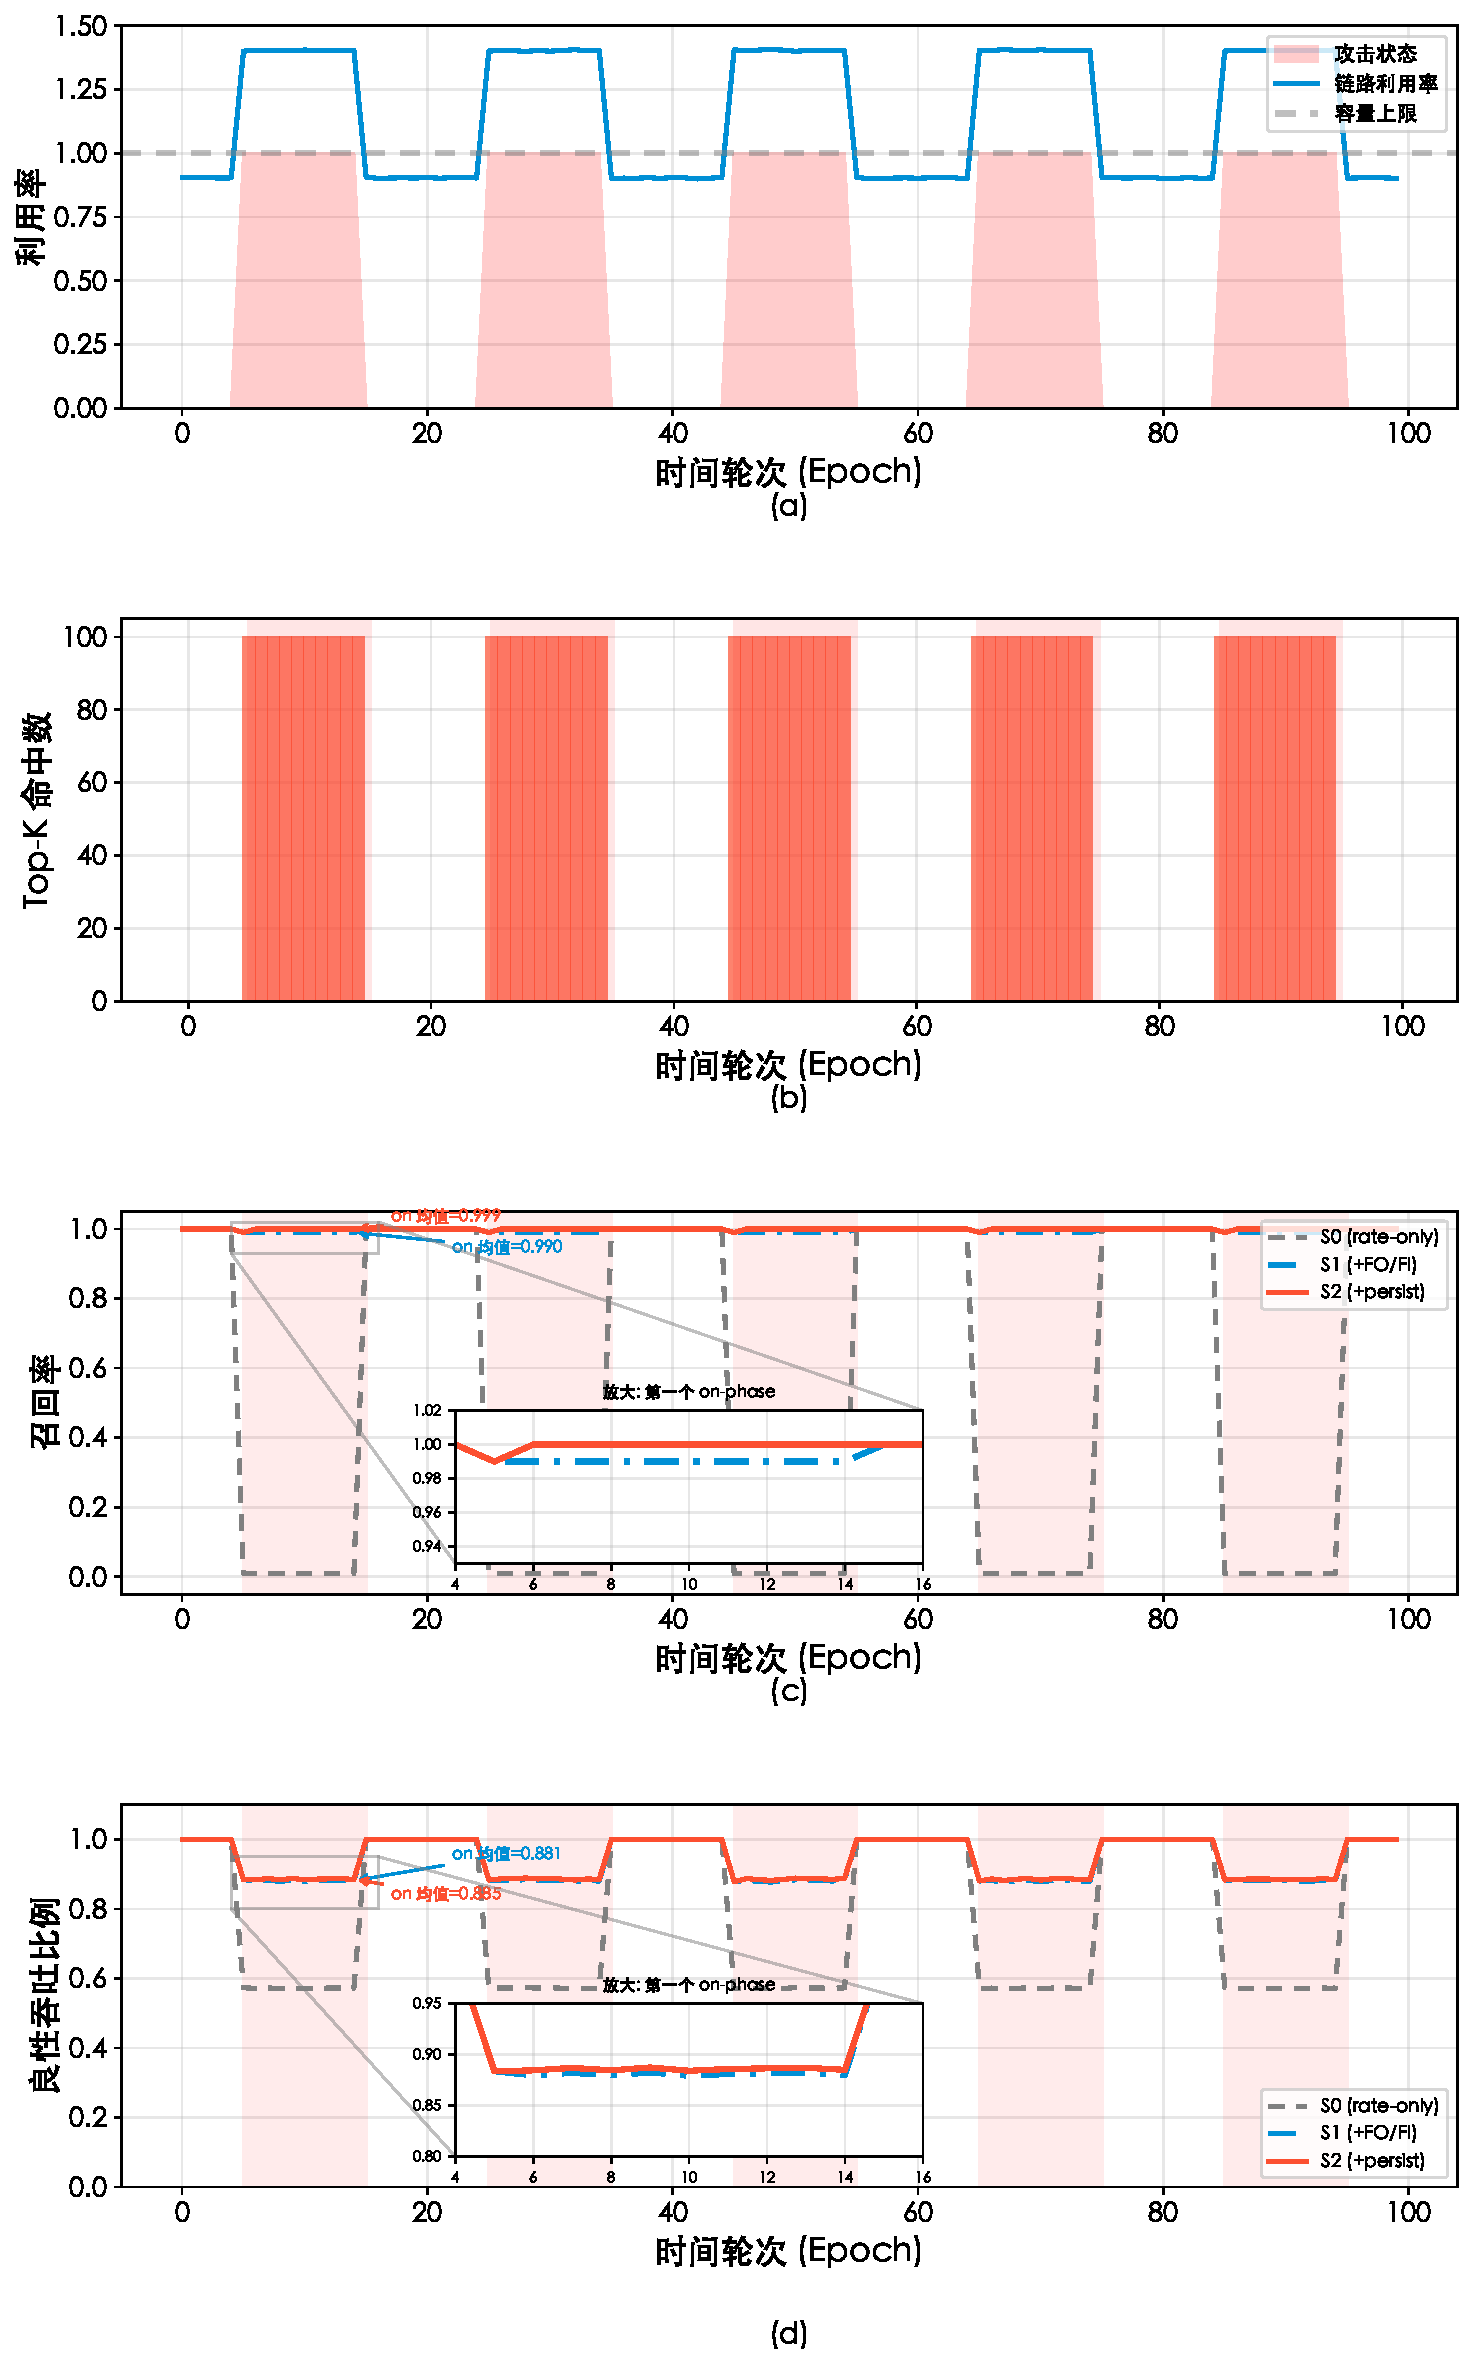
\includegraphics[width=0.94\linewidth]{figs/ch3/fig3_4_onoff.pdf}
  \caption{脉冲式 on-off 攻击下的时域响应对比（$M=100$）。红色阴影表示攻击 on-phase；(a) 目标链路利用率随 epoch 的变化；(b) 一级候选命中的攻击 key 数量；(c) S0、S1、S2 三种方案的 Recall 时域曲线；(d) 三种方案下良性吞吐比例的时域曲线。S2 通过持续性加性奖励与历史候选扩展机制，在候选抖动处保持了更平滑、更高的检测与吞吐保护效果。}
  \label{fig:ch3_fig4_attackstate}
\end{figure}

图~\ref{fig:ch3_fig4_attackstate} 的结果较为清楚。图~\ref{fig:ch3_fig4_attackstate}(a) 表明，攻击 on-phase 到来时目标链路利用率迅速升至超载区间，off-phase 又回落至正常水平，说明该设定确实对应时域上的动态退化，而不是前文的静态退化场景。图~\ref{fig:ch3_fig4_attackstate}(b) 则表明，一级候选集在 on/off 切换附近存在明显抖动：on-phase 内命中数接近攻击 key 总数，但在切换边界处会短暂回落，这正是持续性特征要补偿的部分。进一步看检测结果，图~\ref{fig:ch3_fig4_attackstate}(c) 中 S0 在 $M=100$ 下几乎完全失效（on-phase 平均 Recall$\approx0.01$）；S1 借助 FO/FI 可以实现高召回检测（on-phase 平均 Recall$\approx0.990$），但在切换边缘仍会因候选抖动出现轻微波动；S2 则进一步将 on-phase 平均 Recall 提升到 $0.999$。这里还需说明，off-phase 不存在攻击 key，Recall 按空真值 convention 记为 $1.0$，仅用于保持时域曲线连续。

S2 的提升来自两个机制叠加。持续性采用加性奖励权重（$\alpha=\beta=0.5$, $\gamma=0.2$），即 $\gamma$ 作为额外加分而不从基础权重中借用，因此 S2 的基础检测能力与 S1 保持一致。与此同时，当 $\gamma>0$ 时，系统会将历史上 $P\geq2$ 但未进入当前一级候选集的 key 也纳入评分候选集（见算法~\ref{alg:ms_satshield} 中的持续性扩展步骤），从而为短暂跌出候选集的可疑 key 保留一段记忆。这个机制在缓解侧也有体现：图~\ref{fig:ch3_fig4_attackstate}(d) 显示 S0 的良性吞吐仅为 $0.572$，S1 恢复到 $0.881$，S2 进一步提升到 $0.885$。此外，由于本文取 $k_p=5$，在 off 持续 $10$ 个 epoch 后，所有攻击 key 的 $P_t(a)$ 都会衰减为 $0$，持续性分数随之归零，因此不会把历史攻击残留带入后续判决。

从时域角度看，S2 的改进也主要集中在 on/off 边界，而不是稳态阶段。换句话说，persist 不会把原本不可分的静态样本变得可分，它做的是用跨 epoch 的弱记忆平滑短时抖动，减少候选短暂丢失带来的性能下降。这与图~\ref{fig:ch3_fig2_f1}(b) 中 S2 在静态场景下几乎没有额外收益的结果是一致的：persist 解决的是时间连续性问题，而不是静态结构可分性问题。这样一来，第三章的方法边界也会更清楚，并能更自然地引出第四章的网络级协同。

\subsection{消融实验与参数敏感性分析}
\label{sec:ch3_eval_ablation}
为进一步说明仅对一级候选维护 FO/FI 时的资源与精度权衡，本节对候选规模 $K$、位图长度 $m$、epoch 长度 $\Delta$ 三个参数进行敏感性实验。实验固定退化设定为 $M=100$（速率特征开始失效的分界点），采用 S1（$\alpha=\beta=0.5$）方案进行评估。

\begin{figure}[!htb]
  \centering
  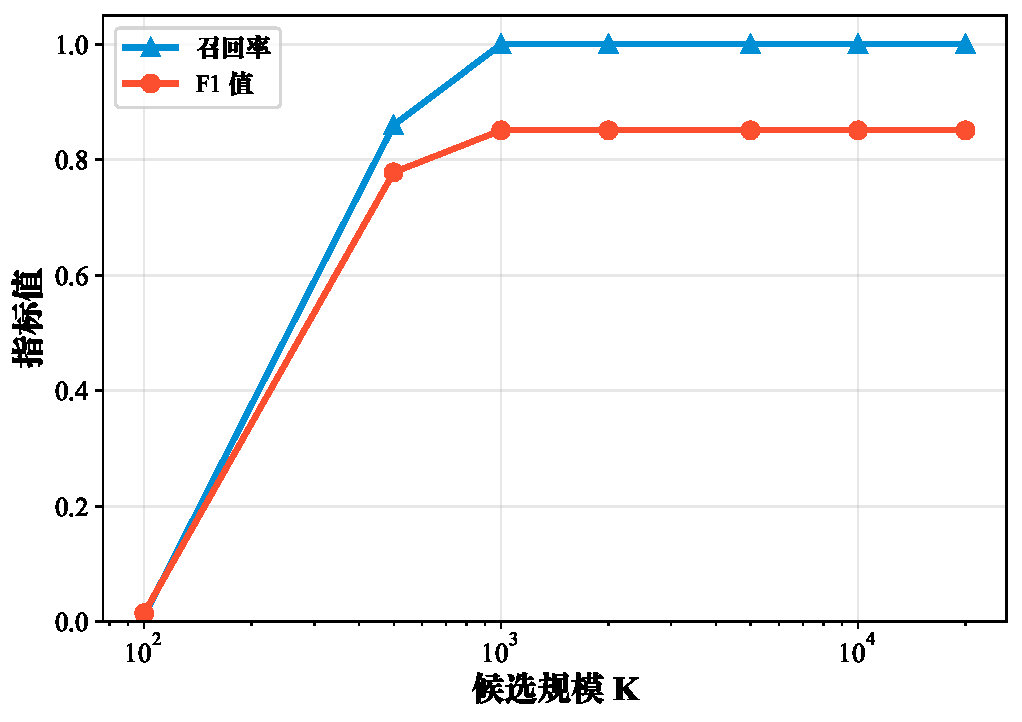
\includegraphics[width=0.65\linewidth]{figs/ch3/ablation_K.pdf}
  \caption{候选规模 $K$ 对 Recall 与 F1 的影响（$M=100$, S1 方案）。$K=1000$ 时 Recall 饱和至 $1.0$，F1 达到约 $0.91$，为推荐的默认值。}
  \label{fig:ch3_ablation_K}
\end{figure}

\noindent\textbf{（1）候选规模 $K$}\quad
图~\ref{fig:ch3_ablation_K} 展示了 Recall 与 F1 随 $K$ 的变化。当 $K<500$ 时，Recall 与 F1 几乎同步上升，这说明此区间内一级候选缓存容量过小，大量攻击 key 尚未进入候选集，是检测性能的主要瓶颈。$K$ 增至 $1000$ 时 Recall 饱和至 $1.0$，F1 达到约 $0.91$。继续增大 $K$（$2000\sim20000$）后 Recall 保持 $1.0$，F1 略有下降（趋近 $0.90$），原因是更多良性 key 涌入候选集增加了误报基数。从资源角度看，若仅计单个 $256$~bit 位图，则 $K=1000$ 时位图本体约为 $K\times m / 8 = 32$~KB；但按本文统一的部署口径，同时计入 CMS 矩阵、候选缓存、FI/FO 双视图、双缓冲位图、字节计数器、rank 表与辅助寄存器后，总状态预算约为 $200$~KB，仍显著低于典型可编程交换机的片上 SRAM 容量。因此 $K\approx1000$（或等效地 $K\approx0.3\cdot N_{\text{keys}}$）是本文实验设置下的经验较优折中。


\noindent\textbf{（2）位图长度 $m$}\quad
图~\ref{fig:ch3_ablation_m} 展示了 FO/FI 估计误差（MAPE）与总内存随 $m$ 的变化。$m=32$ 时 MAPE 约 $4.4\%$，$m=256$ 时降至 $1.1\%$，$m=1024$ 时进一步降至 $0.5\%$。内存开销从 $m=32$ 的约 $20$~KB 线性增长至 $m=1024$ 的约 $700$~KB（$K=1000$ 时）。综合考虑精度与开销，$m=256$ 是本文评估点下经验上较优的折中：MAPE 已降至 $1.1\%$，足以区分攻击 FI（$\geq20$）与良性 FI（$1\sim5$）；按统一部署口径计算，总状态预算约为 $200$~KB，处于可编程交换机可承受范围内。

\begin{figure}[!htb]
  \centering
  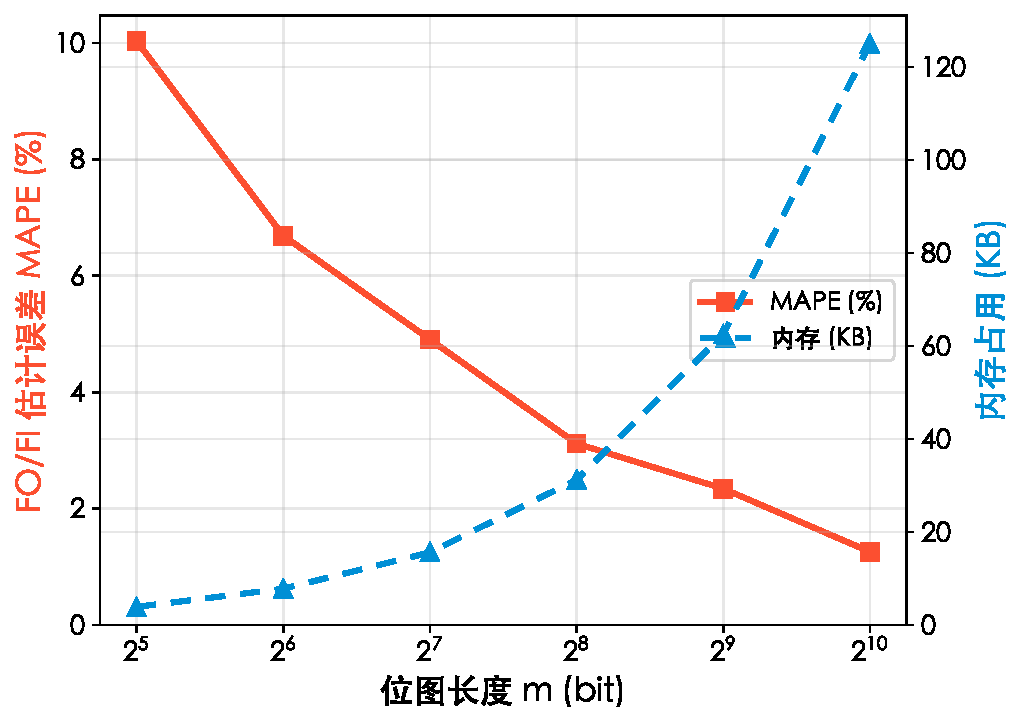
\includegraphics[width=0.65\linewidth]{figs/ch3/ablation_m.pdf}
  \caption{位图长度 $m$ 对 FO/FI 估计误差（MAPE）与总内存的影响（$M=100$, S1 方案）。$m=256$ 时 MAPE 降至 $1.1\%$，内存约 $200$~KB，为推荐的默认值。}
  \label{fig:ch3_ablation_m}
\end{figure}

\noindent\textbf{（3）epoch 长度 $\Delta$}\quad
图~\ref{fig:ch3_ablation_delta} 展示了反应时间与平均良性吞吐下降随 $\Delta$ 的变化。$\Delta=0.1$~s 时反应时间最短（约 $0.2$~s），但代理交互频率高达 $10$ 次/秒，星上计算开销显著增加；$\Delta=5$~s 时反应时间增至 $10$~s，对应良性吞吐下降约 $24\%$。在 $\Delta=0.5\sim1.0$~s 的推荐区间内，反应时间为 $0.5\sim1.0$~s（约 $1\sim2$ 个 epoch），良性吞吐下降约 $12\sim14\%$，系统在响应速度与计算开销之间取得较好平衡。本文选择 $\Delta=1.0$~s 作为默认值。

\begin{figure}[!htb]
  \centering
  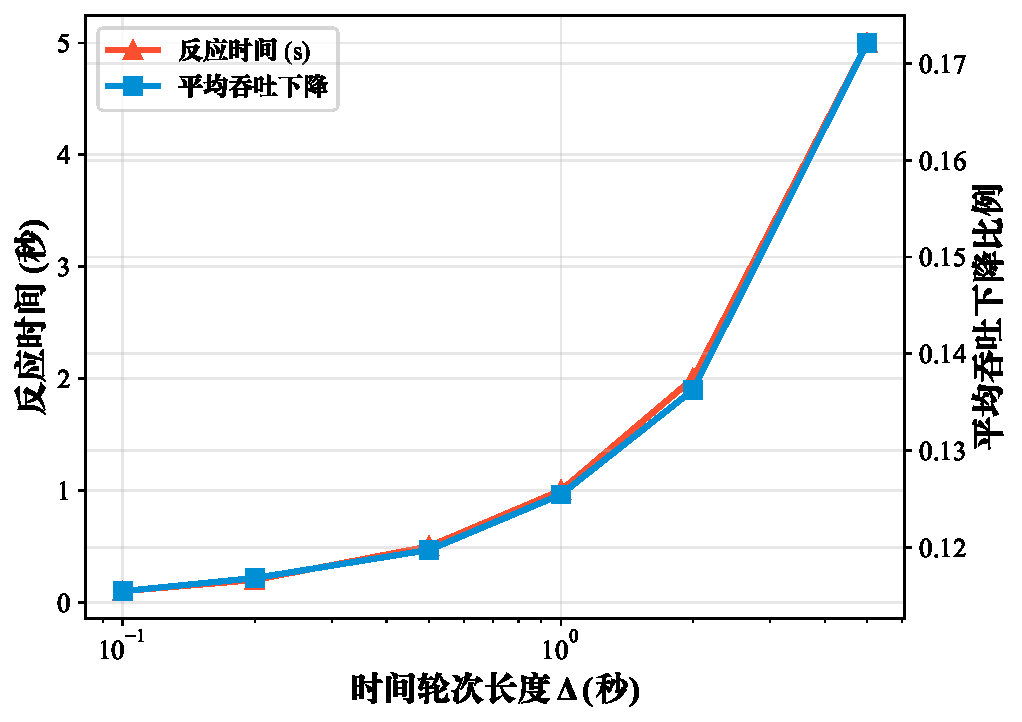
\includegraphics[width=0.65\linewidth]{figs/ch3/ablation_delta.pdf}
  \caption{epoch 长度 $\Delta$ 对反应时间与良性吞吐下降的影响（$M=100$, S1 方案）。$\Delta=1.0$~s 时反应时间约 $1$~s，良性吞吐下降约 $14\%$，为推荐的默认值。}
  \label{fig:ch3_ablation_delta}
\end{figure}

三组消融结果表明，$K$、$m$ 与 $\Delta$ 分别对应三种不同层面的资源约束：$K$ 决定候选覆盖上限，$m$ 决定候选内结构特征的估计精度，$\Delta$ 决定闭环时延与统计稳定性。它们之间并非彼此独立，例如增大 $K$ 会放大位图总开销，缩短 $\Delta$ 会提高 agent 读写频率并加剧候选抖动。因此，本文给出的 $K=1000$、$m=256$、$\Delta=1.0$~s 是面向当前星座规模、链路容量与攻击设定得到的一组经验折中参数。若部署场景发生变化，这三者应被视为联合调参量，而不是彼此孤立的常数。

需要指出的是，地面网络中已经提出了若干针对 LFA 的检测与缓解方案。在 SDN 集中式路线上，Crossfire\citess{crossfire} 利用网络范围内的流量重布局与 SDN 集中控制来检测并解除链路拥塞，Coremelt\citess{coremelt} 利用 NetFlow 分析识别可疑通信对，LinkScope\citess{linkscope} 通过主动探测检测目标链路拥塞，Woodpecker\citess{woodpecker} 和 RADAR\citess{radar} 则分别从路径重路由和相关性分析角度实现 SDN 驱动的 LFA 防御。在可编程数据面路线上，Ripple\citess{ripple} 提出了基于 P4 的去中心化 LFA 防御，Mew\citess{mew} 进一步扩展了 P4 数据面的大规模 LFA 检测能力。然而，这些方案都难以直接应用于 LEO 场景：SDN 集中式方案依赖低时延控制通道与全局视图，而 LEO 的星地和星间控制链路存在明显的时延与带宽限制；P4 方案虽然实现了数据面检测，但依赖地面交换芯片更充裕的片上资源（如 Tofino 2 的 80~MB SRAM），难以满足星载设备的 SWaP 约束。MS-SatShield 的优势在于将检测与缓解逻辑下沉到星载可编程交换机，并在约 $200$~KB 的统一部署状态预算下实现近实时在网缓解。

% [INS-ICARUS-11]
\subsection{方法适用边界与外推限制}
本文方法的第一类边界来自候选覆盖率。实验已经表明，当攻击分散度继续增大（如 $M\geq500$）时，一级候选召回下降会成为主要瓶颈，多签名判别能力也随之受制于候选质量上限。该现象与 ICARUS 在高不确定路由、高分散流量下给出的资源上升但攻击仍可行这一结论并不冲突：二者共同说明，防御侧需要同时改进候选生成与候选内判别，而不能只优化后者\citess{icarus}。

% [INS-ICARUS-12]
第二类边界来自路由策略与网络级目标的差异。本文默认单星本地检测与队列缓解，未显式建模多路径随机负载分担下的概率攻击构造，也未直接评估区域级断连目标。ICARUS 的结果表明，增强路径多样性虽然可以提高攻击成本，但也可能引入显著的时延代价；因此，本文结论应理解为既定路由与本地观测条件下的检测缓解收益，而不应直接外推为全网路由韧性的充分条件\citess{icarus,handley2018delay_not_option,handley2019ground_relays}。

\section{本章小结}
本章针对大规模低轨卫星网络中的链路洪泛攻击，提出了 MS-SatShield 多签名在网检测与队列缓解方法。该方法在 SatShield 的一级候选生成与队列调度框架上，引入 fan-in/fan-out 与持续性等结构性签名，以应对速率特征退化场景；同时通过仅对候选集合维护 FO/FI 的设计，将 distinct 统计的状态成本控制在 $O(K\cdot m)$，并在统一部署口径下将总数据面状态预算控制在约 $200$~KB（默认 $K=1000$, $m=256$，同时计入 CMS 矩阵、候选缓存、FI/FO 双视图、双缓冲位图、字节寄存器与队列映射表等辅助结构）。

实验结果表明：（1）在多 decoy 分摊退化下（$M=100$），仅靠聚合速率的 S0 方案 F1 降至 $0.017$，引入 FO/FI 后的 S1 方案 F1 恢复到 $0.908$；（2）在脉冲式 on-off 攻击下，持续性特征通过加性奖励与候选集扩展机制将 S2 方案的 on-phase 平均 Recall 提升到 $0.999$，良性吞吐恢复到 $0.885$；（3）消融实验表明，在本文评估设置下，$K\approx1000$、$m=256$、$\Delta=1.0$~s 是检测精度与资源开销之间较合适的一组经验折中参数。

不过，上述结果仍局限于单星、单链路视角。当 $M\geq500$ 时，各方案 F1 都下降到 $0.42\sim0.46$，主要受制于单链路一级候选集的覆盖率瓶颈（一级候选 Recall$\sim0.3$）。此外，单节点缓解只是在拥塞形成后于末端丢弃攻击流量，无法阻止攻击流在上游链路上继续消耗带宽。这些局限也自然引出第四章的研究方向：通过多星协同的证据融合与逐跳推回机制，在网络级实现更早、更充分的攻击缓解。



%========================
% 第四章：研究点 2（多星协同在网计算）
% 章节主题：面向大规模低轨卫星网络的抑制型邻居扩散协同与推回缓解
%========================


\chapter{面向大规模低轨卫星网络的多星协同在网计算与推回缓解方法研究}
\label{chap:coop_innetwork}

\section{引言}
\label{sec:ch4_intro}

上一章（\ref{chap:ms_satshield}）讨论了单星、单节点视角下的链路洪泛攻击检测与缓解，利用可编程交换机的数据面线速能力实现了对可疑聚合 key 的实时识别与队列调度缓解。这类星上本地闭环的优势很直接，即不必依赖地面控制器完成统计上报和策略下发，从而避开卫星到地面以及星间控制链路带来的时延开销。在 LEO 星座网络中，这一点尤其重要。现有研究指出，卫星网络控制环路的延迟可达几十毫秒，而攻击流量能够在亚毫秒级完成自适应变化，因此依赖中心控制器的传统 LFA 防御很难跟上快速演化的攻击\citess{satshield}。

然而，只依赖受害链路附近的本地缓解仍有两方面不足。本地缓解往往发生在拥塞已经形成之后，攻击流量在到达目标瓶颈链路前，已经沿多条星间链路消耗了大量带宽和队列资源。这种末端丢弃会在网络内部制造额外拥塞风险，也会明显放大对良性业务的影响。另一方面，LEO-LFA 攻击具有明显的全网性与漂移性。攻击者可以利用公开的轨道和拓扑信息，结合低时延路由偏好带来的路径可预测性，在全球范围内灵活选择 bot 分布和攻击路径，使攻击证据以碎片化形式分散在多个卫星节点上\citess{icarus}。在这种情况下，即使单个节点具备较强的本地检测能力，缺乏跨节点信息共享仍会限制整体缓解效果。各节点只能在本地丢弃已经到达的攻击流量，难以把抑制动作前推到更靠近攻击源头的上游节点，结果就是大量链路带宽被白白占用。


% [INS-2026-CH4-01]
2025--2026 年的产业实践也让多星协同的必要性更加明确。Starlink 通过 Stargaze 在星座内部形成空间态势感知能力，OneWeb 将自动化避碰纳入运营流程，Direct to Cell 与企业私网业务又使同一套卫星网络同时承载更强的连续性和关键业务保障要求\citess{spacex_stargaze_2026, eutelsat_responsible_space_2026, starlink_direct_to_cell_2026, amazon_leo_enterprise_2025, eu_iris2_2024}。在这一背景下，只在受害点附近做本地限速已经难以满足星座的自治需求。防御系统需要在邻近卫星之间快速交换证据，并把抑制动作前移到更上游的位置，使其能够和轨道侧其他自治闭环并行工作。多星协同与逐跳推回因此不再只是性能优化，而是与星座运行方式相匹配的防御需求。

从系统条件看，LEO 星座网络本身具备开展多星协同在网计算的基础。典型星座的星间连接度较低，例如 Starlink Shell 1 中每颗卫星通常配置 4 条 ISL，单条 ISL 的容量可达 20~Gb/s 量级\citess{icarus}。与此同时，星座拓扑和最短路结构的变化发生在秒级时间尺度上，因此可以将系统近似为一系列稳定的拓扑快照并分时处理\citess{icarus}。此外，卫星节点也在逐步演进到全栈可编程架构，已经具备在数据面执行轻量计算、在星上 agent 执行局部控制的条件\citess{satshield}。基于这些条件，本章提出一种面向大规模 LEO 的\textbf{抑制型邻居扩散协同（suppressed gossip）}与\textbf{推回缓解（pushback）}机制，在不依赖地面中心控制器的前提下，实现跨卫星的攻击证据聚合以及更靠近源头的分布式缓解，并通过区域限制、抑制扩散和速率配额来避免大规模网络中的信令风暴。

本章主要做了三件事。首先，给出本地证据抽取、协同证据聚合和推回缓解执行组成的多星协同在网计算框架，将上一章的本地检测能力扩展到网络级威胁判断。其次，设计面向大规模星座的抑制型邻居扩散协议，在尽量保持协同收敛速度的同时降低控制信令开销。最后，在 Starlink Shell 1 拓扑和真实流量背景（CAIDA trace）下完成系统实现与实验评估，量化展示其相对 NoDefense、SatShield 和 MS-SatShield 三类星载基线的缓解收益。至于 LinkScope、Woodpecker、RADAR、Ripple 与 Mew 等地面 LFA 防御方案，本文仍将它们保留为设计参照和假设差异的讨论对象，但不把它们作为正文图表中的数值基线\citess{satshield,icarus,linkscope,woodpecker,radar,ripple,mew}。

\section{基于抑制型邻居扩散的多星协同在网计算方法}
\label{sec:ch4_method}

\subsection{问题模型与设计目标}
\label{subsec:ch4_model_goal}

\noindent\textbf{（1）时变星座与拓扑快照假设}\quad
将LEO星座表示为时变图$G(t)=(V(t),E(t))$。由于卫星运动导致的最短路径变化发生在秒级时间尺度\citess{icarus}，本章采用离散epoch建模：在epoch长度$\Delta$内，近似认为拓扑与路由策略不变，记为$G_\tau$（$\tau$为epoch索引）。该假设与 ICARUS 按快照预计算攻击流分配的对手能力一致\citess{icarus}，也与 SatShield 在星上闭环配置 agent 的周期更新机制相兼容\citess{satshield}。

\noindent\textbf{（2）威胁模型与推回收益}\quad
攻击者控制分布在全球范围的bot集合，生成看似合法的低速流量，并通过精心选择源-目的对使攻击流聚合在目标ISL上形成拥塞\citess{crossfire, icarus}。设目标瓶颈链路为$e^\*$，其容量为$C_{e^\*}$；攻击流量在该链路处的聚合速率为$A$，则拥塞发生条件近似为$B + A > C_{e^\*}$（$B$为背景流量）。为了刻画末端丢弃对网络内部资源的消耗，本章将$W_{\text{waste}}$定义为\emph{路径积分意义下的无效带宽占用成本}：对epoch $\tau$内的攻击相关key集合$\mathcal{A}^{\text{atk}}_\tau$，记key $a$在被首次限速/丢弃之前所经历的链路集合为$P_\tau(a)$，其在链路$e\in P_\tau(a)$上的聚合速率为$x_{a,e}(\tau)$，则
\begin{equation}
W_{\text{waste}}(\tau)=\sum_{a\in\mathcal{A}^{\text{atk}}_\tau}\ \sum_{e\in P_\tau(a)} x_{a,e}(\tau),\qquad [W_{\text{waste}}]=\text{Mb/s}\cdot\text{hop}.
\label{eq:waste_bw}
\end{equation}
该定义从防御者视角将攻击流在网络中占用的每一跳链路资源都计入无效成本，因此与后文图示中的$\text{rate}\times h$以及柱状图使用的 Mb/s$\cdot$hop 量纲保持一致。若进一步假设各 key 沿路径上的速率近似恒定，且攻击流的平均承载跳数为$\bar h$，则式\eqref{eq:waste_bw}可近似写为
\begin{equation}
W_{\text{waste}}(\tau) \approx \bar h\cdot A.
\label{eq:waste_bw_approx}
\end{equation}
若只关心受害链路上游的额外浪费，可以在式\eqref{eq:waste_bw}基础上减去目标链路上的聚合速率$A$；但为了与后文图示和实验统计保持一致，本文统一采用式\eqref{eq:waste_bw}给出的全路径积分口径。在 Starlink Shell 1 中，ISL 容量约为 20~Gb/s\citess{icarus}，而 ICARUS 与 SatShield 都表明，攻击者在数百到数千 bot 规模下即可形成可观的攻击带宽\citess{icarus,satshield}。因此，即使$\bar h$取较小常数，$W_{\text{waste}}$仍可能达到数十 Gb/s$\cdot$hop 量级，并进一步引发更广泛的链路排队与连锁拥塞。推回收益能够用这一指标直接度量，这也是本章引入多星协同与 pushback 机制的直接动机。

\noindent\textbf{（3）设计目标}\quad
在上述模型下，本章主要关注三个目标。首先是快速性，协同判断与 pushback 传播需要在攻击自适应时间尺度之前完成闭环更新，避免再次落回中心控制器的高时延反馈环\citess{satshield}。其次是可扩展性，当星座规模达到数千甚至上万颗卫星时，协同机制不能采用全网广播式信令，控制开销应远小于 ISL 带宽，并且保持数据面可实现。最后是稳健性，面对分散化、低速化、脉冲化和滚动目标等攻击策略，协同机制需要把碎片化证据汇聚成网络级信号，减少本地 top-$k$ 漏检对整体防御效果的影响。这个问题在\ref{chap:ms_satshield}中已经通过退化设定作过论证。

\subsection{系统总体架构：CoopSatShield}
\label{subsec:ch4_arch}

为实现上述目标，本章提出多星协同在网计算系统\textsc{CoopSatShield}。系统由本地证据抽取（Local Evidence）、抑制型邻居扩散协同（Suppressed Gossip）和推回缓解执行（Pushback Enforcement）三部分构成。体系结构如图~\ref{fig:ch4_arch}所示。

图~\ref{fig:ch4_arch}左侧展示了单颗卫星节点$v$的内部架构，右侧展示了多节点协同拓扑。

\textbf{单节点内部架构}（图~\ref{fig:ch4_arch}左栏）分为上下两层：下层为面向 P4 可编程交换机\citess{bosshart2014p4} 的数据面快路径，上层为星上 Agent（控制面，以 epoch 为周期）。

数据面包含 6 个模块，可分为复用模块与新增模块两组：
\begin{enumerate}
\item \textbf{复用模块}（Ch.3 MS-SatShield）：CMS 与候选缓存组成的一级候选生成，用于维护候选 key 集合及其近似频次；FO/FI 位图，用于记录候选 key 的扇出或扇入结构特征；队列调度，用于基于 rank 执行优先级队列映射与限速。
\item \textbf{新增模块}（$\star$~Ch.4）：入端口贡献统计，用于维护每个候选 key 在各入端口的字节统计$\text{bytes}(a,p)$，供后续 pushback 选择上游；EG/PT 消息解析，用于完成协同消息的轻量级 header 解析与 TTL 递减；seen-set 去重，用 Bloom Filter\citess{bloom1970space}实现 O(1) 消息去重。
\end{enumerate}
上述模块在设计语义上都可以映射到可编程交换机的寄存器阵列与 match-action 表\citess{bosshart2013rmt}，每包处理保持 O(1) 复杂度。

控制面 Agent 包含 6 个模块：
\begin{enumerate}
\item 多签名评分（复用 Ch.3），计算候选 key 的多维可疑性评分；
\item 证据缓存$\mathcal{E}_{v,\tau}$，存储 ROI 内接收到的 EG 消息；
\item 抑制型扩散决策，执行冗余抑制判断（$cnt \ge k$时抑制发送）；
\item 协同聚合$S^{\text{net}}$，计算网络级加权评分（式\eqref{eq:net_score}）；
\item Pushback 判定，比较$S^{\text{net}}$与阈值$\Theta_{\text{pb}}$并触发推回；
\item EG 消息处理与合并，执行 Aggregate 操作并构造聚合消息。
\end{enumerate}
两层之间通过 epoch 读取和写回接口连接。Agent 每个 epoch 从 CMS/候选缓存摘要、FO/FI 位图以及入端口贡献表中拉取数据，计算多签名评分后，再将 rank 及推回规则写回数据面。

\textbf{多节点协同拓扑}（图~\ref{fig:ch4_arch}右栏）展示了 7 颗卫星组成的局部拓扑。当节点$V$检测到受害链路$e^*$拥塞时，会触发 EG 消息向外扩散（蓝色箭头，TTL 每跳递减），在 ROI（$R=4$）范围内完成证据共享与聚合；同时，PT 令牌沿贡献最大的上游方向反向传播（橙色箭头，$R_{\uparrow}$递减），沿途节点安装软状态缓解规则。图中也标出了抑制机制的效果：当某节点在发送窗口内已经监听到$k$条等价证据时，就会抑制本次转发，避免冗余广播。

\begin{figure}[!htb]
\centering
\includegraphics[width=0.95\linewidth]{figs/ch4/fig4_arch_TODO.pdf}
\caption{\textsc{CoopSatShield}体系结构。左栏：单节点内部架构，上层为星上Agent（控制面），下层为P4可编程交换机（数据面），标注Ch.3复用模块与Ch.4新增模块（$\star$）。右栏：多节点协同拓扑，EG消息向外扩散（蓝色）与PT令牌向上游推回（橙色），虚线圆标注ROI边界。}
\label{fig:ch4_arch}
\end{figure}

\subsection{本地证据抽取与证据单元构造}
\label{subsec:ch4_local_evidence}

本节复用\ref{chap:ms_satshield}的本地多签名检测流水线，并将其输出进一步组织为可协同处理的证据单元。对协同计算而言，节点输出不仅要给出硬判定结果，还需要便于聚合、比较和传播抑制。基于这一要求，本节定义如下证据结构。

对卫星$v$在epoch $\tau$内的某条出端口链路$e=(v,u)$，定义其拥塞指示量为：
\begin{equation}
c_{v,e}(\tau) = \mathbf{1}\big[q_{v,e}(\tau) > Q_{\text{th}} \ \vee \ d_{v,e}(\tau) > D_{\text{th}}\big],
\label{eq:cong_indicator}
\end{equation}
其中$q_{v,e}(\tau)$表示该端口的队列占用（或排队时延估计），$d_{v,e}(\tau)$表示端口丢包率（或 RED/ECN 触发率），$Q_{\text{th}},D_{\text{th}}$为阈值。该指标完全来自数据面或交换机 traffic manager 的可观测量，符合星上实时性要求。为了便于后续权重计算，本章进一步定义归一化的拥塞等级：
\begin{equation}
\texttt{cong\_level}_{v,e}(\tau)=\min\!\left(1,\max\!\left\{\frac{q_{v,e}(\tau)}{Q_{\text{th}}},\ \frac{d_{v,e}(\tau)}{D_{\text{th}}}\right\}\right)\in[0,1].
\label{eq:cong_level}
\end{equation}
其中$Q_{\text{th}},D_{\text{th}}$直接继承第\ref{chap:ms_satshield}章的数据面拥塞告警配置，本章只复用其部署阈值，不把它们作为新的调参维度；若节点在同一 epoch 内观测到多条拥塞链路，则在式\eqref{eq:weight}中取相应$\texttt{cong\_level}_{v,e}(\tau)$的最大值作为节点级拥塞强度。

当$c_{v,e}(\tau)=1$时，节点$v$从本地候选集$\mathcal{H}_{v,\tau}$中提取与链路$e$最相关的 top-$n$ 可疑 key 集合$\mathcal{A}_{v,e,\tau}$，并为每个$a\in\mathcal{A}_{v,e,\tau}$给出本地多签名评分$S_{v,\tau}(a)$（见\ref{chap:ms_satshield}式( \ref{eq:score_def} )）。与此同时，还输出该 key 在不同入端口上的贡献分布$\pi_{v,\tau}(a)$，供后续 pushback 选择上游：
\begin{equation}
\pi_{v,\tau}(a,p)=\frac{\text{bytes}_{v,\tau}(a,p)}{\sum_{p'}\text{bytes}_{v,\tau}(a,p')},
\label{eq:ingress_contrib}
\end{equation}
其中$p$为$v$的入端口编号，$\text{bytes}_{v,\tau}(a,p)$为 epoch 内从端口$p$进入且匹配 key $a$ 的字节数。由于 LEO 星间连接度较低（典型为 4 条 ISL 加地面链路）\citess{icarus}，这一分布统计可以在有限状态下实现，也能直接用于识别攻击流主要来自哪个上游邻居。

\subsection{抑制型邻居扩散协同：避免信令风暴的gossip设计}
\label{subsec:ch4_gossip}

\subsubsection*{（1）为何需要抑制机制}
在大规模星座中，朴素 gossip 的做法是每个 epoch 内每个节点都向所有邻居发送摘要并继续转发，这会使控制信令随网络规模快速增长。即使单条消息本身很小，当$|V|$达到数千时，持续扩散仍会带来不必要的链路占用和处理负担，更严重的是会在拥塞期间与数据业务争抢资源，出现防御信令反过来挤压业务的情况。LEO 网络的一个重要特征在于，攻击影响通常集中在受害链路及其上游汇聚路径附近，因此协同传播也应局部化、事件驱动，并且能够抑制重复传播。

本章用三种约束来控制信令扩散。首先采用事件驱动，只有当$c_{v,e}(\tau)=1$或接收到新颖证据时才触发发送；其次采用区域限制，让每条证据消息携带 TTL，最多传播$R$跳，从而形成受影响区域 ROI；最后采用抑制扩散，借鉴传感网中的冗余抑制思想\citess{demers1987epidemic}，当节点在一个发送周期内已经听到足够多重复证据时，就自动抑制自身转发，避免扩散规模持续膨胀。这里的实现接近 Trickle 协议\citess{levis2004trickle}的抑制思想，但并不沿用其倍增窗口机制，而是采用固定时隙$I$来简化星上实现。

\subsubsection*{（2）协同消息类型与格式}
本章定义两类星间控制消息：证据扩散消息（Evidence Gossip, EG）与推回令牌（Pushback Token, PT）。其中EG负责传播与聚合证据，PT负责执行缓解推回。表~\ref{tab:msg_format}给出EG消息字段。

\begin{table}[t]
\centering
\caption{Evidence Gossip（EG）消息字段设计}
\label{tab:msg_format}
\begin{tabular}{l|l}
\hline
字段 & 含义 \\
\hline
$\texttt{type}$ & 消息类型标识（4-bit），用于区分EG与PT \\
$\texttt{epoch}$ & 当前epoch编号，用于软状态一致性与过期清理 \\
$\texttt{link\_id}$ & 触发拥塞的链路标识（如$(v,u)$或端口号） \\
$\texttt{ttl}$ & 剩余传播跳数（ROI半径$R$） \\
$\texttt{nonce}$ & 消息唯一标识，用于去重缓存（seen-set） \\
$\texttt{digest}$ & 候选key集合摘要（例如Bloom Filter），用于快速交集判断 \\
$\langle \widehat{a_i}, \widehat{s_i}\rangle_{i=1}^{n}$ & top-$n$可疑key的哈希表示与量化评分 \\
$\texttt{cong\_level}$ & 按式\eqref{eq:cong_level}归一化得到的拥塞等级 \\
\hline
\end{tabular}

\end{table}

\begin{table}[t]
\centering
\caption{Pushback Token（PT）消息字段设计}
\label{tab:pt_format}
\begin{tabular}{l|l}
\hline
字段 & 含义 \\
\hline
$\texttt{type}$ & 消息类型标识（4-bit），用于区分EG与PT \\
$\texttt{epoch}$ & 触发epoch编号，用于软状态一致性 \\
$R_{\uparrow}$ & 剩余推回跳数（4-bit），每跳递减直至0终止 \\
$\texttt{key\_hash}$ & 目标key的CRC32短哈希$\widehat{a}$（32-bit） \\
$\texttt{rank}$ & 缓解优先级（8-bit：High/Med/Low，映射到队列与限速） \\
$T_{\text{life}}$ & 软状态生存期（8-bit，以epoch为单位），到期自动清除 \\
\hline
\end{tabular}
\end{table}

其中$\widehat{a_i}$为 key 的 CRC32 短哈希（32-bit），在实际 key 空间中碰撞率很低，同时能够节省带宽；$\widehat{s_i}$为量化评分（8-bit，线性映射$[0,1]$至$[0,255]$），分辨率$1/256$已足够完成排序和阈值判断。默认配置下，$\texttt{digest}$采用 128-bit Bloom Filter\citess{bloom1970space}编码候选 key 集合，接收端可以用 O(1) 代价判断本地候选是否与对方证据存在重叠，也就是对式\eqref{eq:overlap}中$\Omega$进行快速近似，从而避免对无关证据执行高代价合并。该默认配置对应图中的消息格式与大小统计。

图~\ref{fig:ch4_header} 用 bit-level 字段图展示了两类协同控制消息在\textbf{默认配置}下的具体格式。EG 消息的固定头部由 $\texttt{type}$（4-bit）、$\texttt{epoch}$（16-bit）、$\texttt{ttl}$（4-bit）、$\texttt{nonce}$（32-bit）、$\texttt{link\_id}$（32-bit）、$\texttt{digest}$（128-bit）和 $\texttt{cong\_level}$（8-bit）组成，共 224~bit，即 28~字节，可在 P4 交换机 parser 中以固定偏移完成线速解析；可变载荷部分每个 entry 占 5~字节（$\widehat{a_i}$ 32-bit + $\widehat{s_i}$ 8-bit），图中按默认 $n=10$ 示意，因此单条 EG 消息为 78~字节。PT 消息更紧凑，固定仅\textbf{72~bit（9~字节）}，字段顺序为 $\texttt{type}$、$\texttt{epoch}$、$R_\uparrow$、$\texttt{key\_hash}$、$\texttt{rank}$ 与 $T_\text{life}$，只携带执行缓解所需的最少信息。图下方的 ISL 传播路径示意展示了 EG 沿 TTL 递减方向向外扩散，并在中继节点执行 digest 重叠检查与抑制发送；PT 则沿$R_\uparrow$递减方向反向推回并在沿途节点安装缓解规则。右下角的消息大小对比仅比较默认 EG（$n=10$）与 PT，说明 PT 的开销显著更小。

\begin{figure}[!htb]
\centering
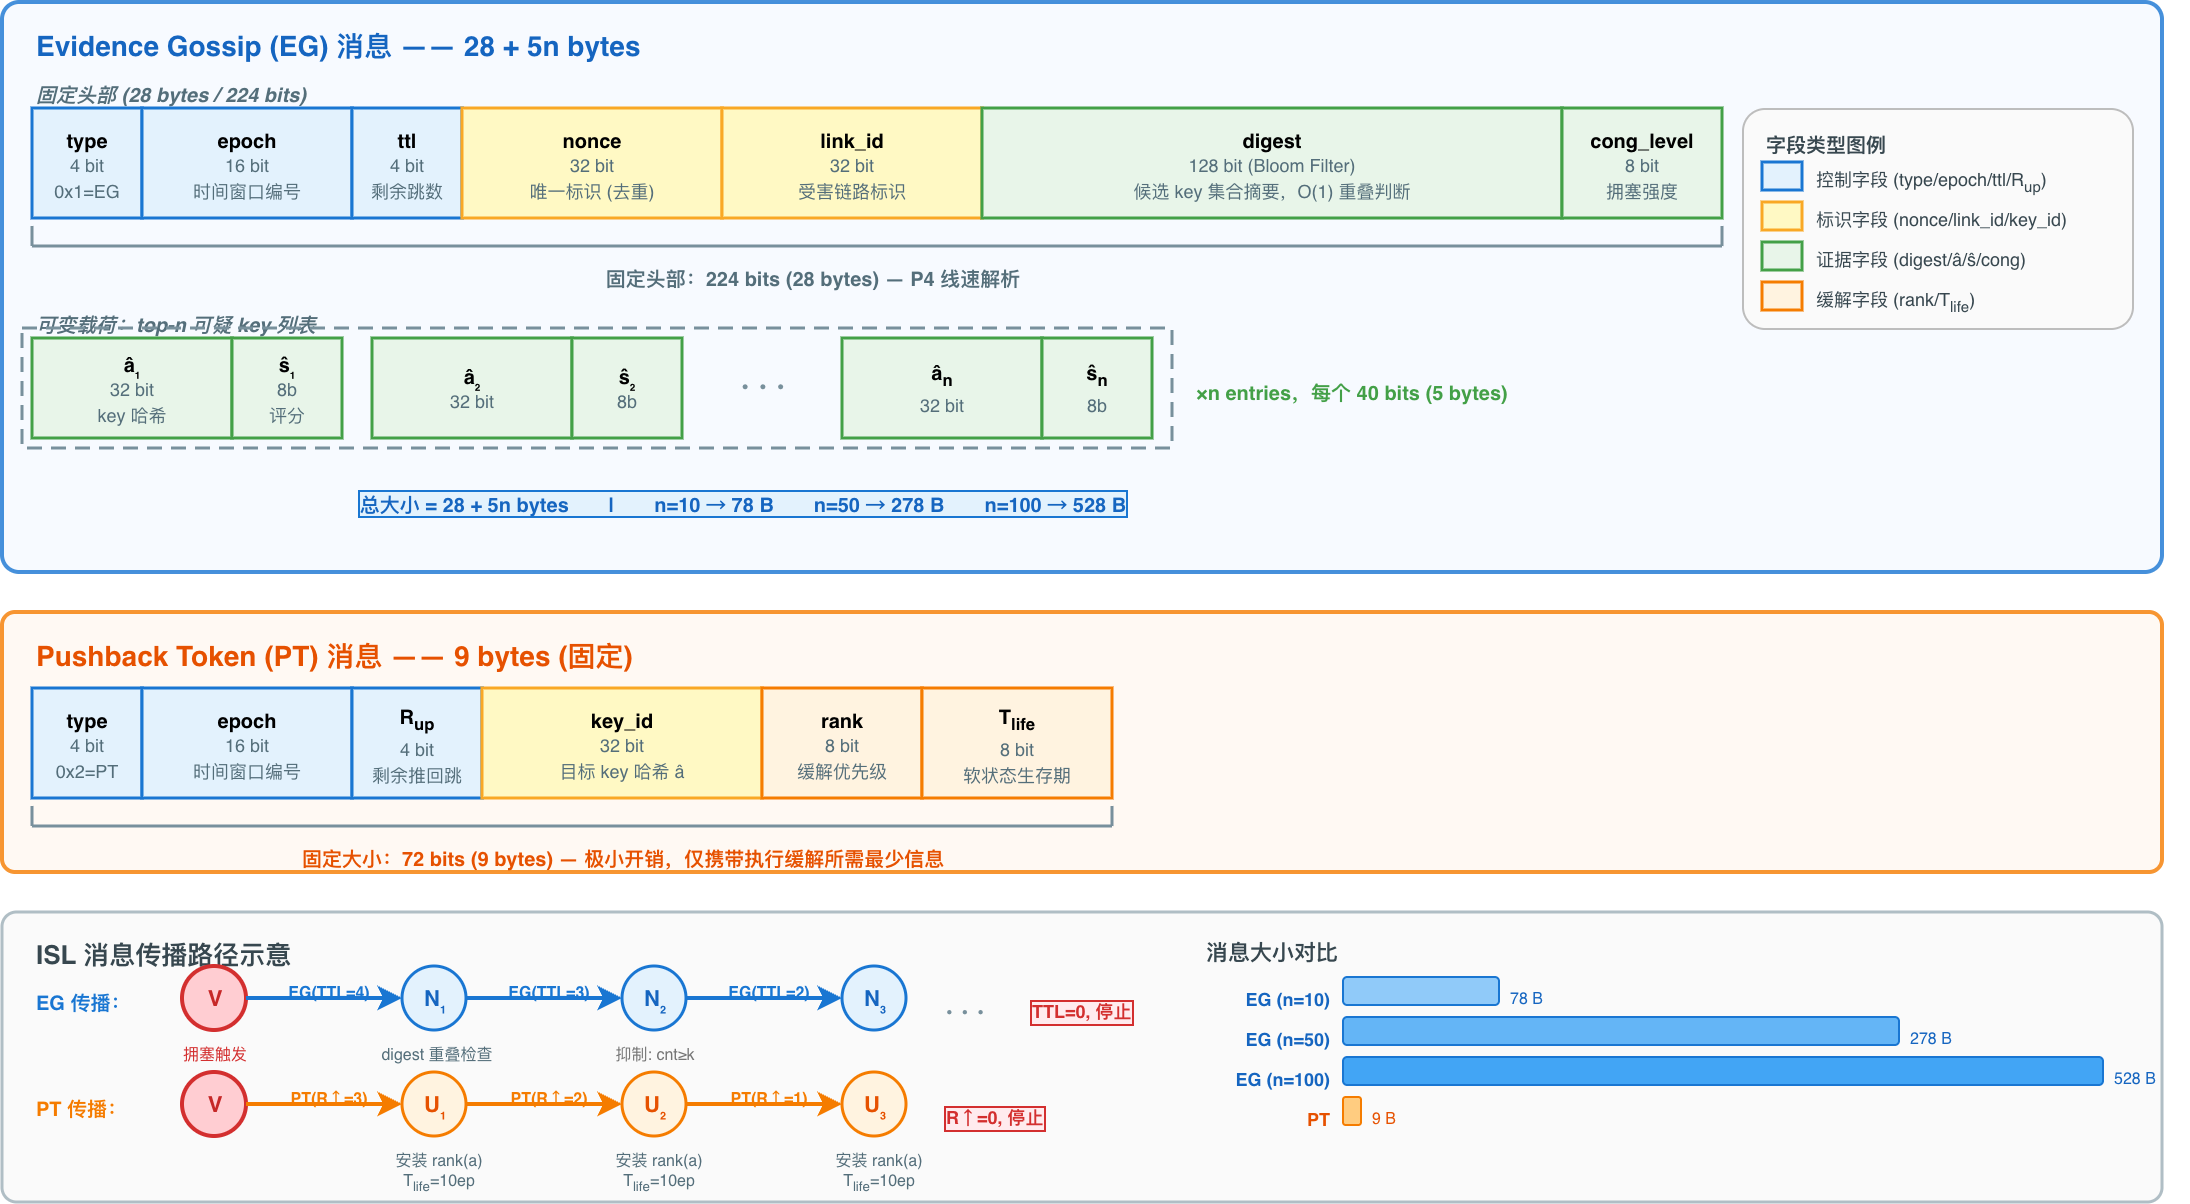
\includegraphics[width=0.92\linewidth]{figs/ch4/fig4_header.png}
\caption{\small 默认配置下的协同控制消息格式。上部：Evidence Gossip（EG）消息，固定头部 28~字节、可变载荷为 top-$n$ 可疑 key 列表，图中按默认 $n=10$ 绘制；字段按功能类型配色（蓝色=控制、黄色=标识、绿色=证据、橙色=缓解）。中部：Pushback Token（PT）消息，72~bit（9~字节）定长。下部：EG/PT 在 ISL 上的传播路径示意，以及默认 EG（$n=10$）与 PT 的消息大小对比。}
\label{fig:ch4_header}
\end{figure}

\subsubsection*{（3）抑制型扩散协议（Suppressed Gossip Protocol）}
设节点$v$在 epoch $\tau$内维护一个证据缓存$\mathcal{E}_{v,\tau}$，存储 ROI 内观察到的 EG 消息摘要。对任意$(\tau,\texttt{link\_id})$，节点以固定时隙$I = \Delta/4$执行一次抑制型扩散，即每个 epoch 内最多执行 4 轮扩散，且$I \ll \Delta$足以保证在 epoch 结束前完成收敛。其基本过程是：节点先在$I$内随机选择一个发送时刻$t_{\text{send}}$；若在$t_{\text{send}}$之前已经监听到至少$k$条等价证据（同一 epoch、同一 link\_id 且 digest 高度相似），则抑制本次发送；否则就在$t_{\text{send}}$发送聚合后的 EG 消息。通过随机化发送时机和冗余抑制，系统可以在保持传播速度的同时减少重复广播。

进一步地，为保证传播局部化，本章规定 EG 消息只有在满足相关性门限时才会继续转发。节点$v$收到来自邻居$u$的 EG 消息$M$后，计算其与本地候选集合$\mathcal{A}_{v,\tau}$的重叠度：
\begin{equation}
\Omega(M,v) = \frac{|\mathcal{A}_{v,\tau}\cap \mathcal{A}(M)|}{|\mathcal{A}(M)|},
\label{eq:overlap}
\end{equation}
其中$\mathcal{A}(M)$表示消息中的 top-$n$ key 集合。只有当$\Omega(M,v)\ge \theta_\Omega$或本地链路同样处于拥塞态$c_{v,e}(\tau)=1$时，节点才会将该证据纳入缓存并参与后续转发。这个机制借助本地观测的一致性过滤无关扩散，是控制信令规模的重要一环。

算法~\ref{alg:suppressed_gossip}给出了抑制型扩散协议的流程。与朴素 gossip 相比，这里的重点不在于能否传播，而在于结合物理网络的局部性和低度数结构，把传播范围控制在 ROI 内，并尽量避免同一证据在区域内反复回旋。

\begin{algorithm}[t]
\caption{抑制型邻居扩散协同（Suppressed Gossip Protocol）}
\label{alg:suppressed_gossip}
\Input{(1) 当前 epoch $\tau$ 的本地拥塞状态 $c_{v,e}(\tau)$ 与本地 EG 候选消息 $M_v$；\newline
(2) 节点状态：证据缓存 $\mathcal{E}_{v,\tau}$ 与发送窗口 $I$；\newline
(3) 协同参数：ROI 半径 $R$、抑制参数 $k$、重叠阈值 $\theta_\Omega$。}
\Output{节点本轮的发送结果 $O_v$：聚合 EG 消息 $\widetilde{M}_v$ 或抑制决策 \textsc{Suppress}。}
\BlankLine
\tcc{步骤 1：本地拥塞触发并启动抑制发送窗口}
初始化发送结果 $O_v\leftarrow \textsc{Suppress}$\;
若存在链路$e$使$c_{v,e}(\tau)=1$，构造本地EG候选消息$M_v$\;
将$M_v$加入缓存$\mathcal{E}_{v,\tau}$，并进入抑制发送窗口$I$\;
在窗口$I$内随机选择$t_{\text{send}}$\;
\BlankLine
\tcc{步骤 2：监听邻居消息并合并等价证据}
\While{$t < t_{\text{send}}$}{
    监听邻居EG消息$M_u$\;
    \If{$M_u$未去重（nonce未见过）且$M_u.\texttt{ttl}>0$}{
        计算$\Omega(M_u,v)$（可由digest快速近似）\;
        \If{$\Omega(M_u,v)\ge \theta_\Omega$ \textbf{or} 本地存在拥塞链路}{
            将$M_u$合并入$\mathcal{E}_{v,\tau}$（top-$n$合并$+$digest并集）\;
        }
    }
}
统计窗口$I$内等价证据数量$cnt$\;
\BlankLine
\tcc{步骤 3：根据冗余程度决定转发或抑制}
\eIf{$cnt < k$}{
    生成聚合消息$\widetilde{M}_v = \texttt{Aggregate}(\mathcal{E}_{v,\tau})$\;
    设置$\widetilde{M}_v.\texttt{ttl}\leftarrow \min(\texttt{ttl}_{\text{received}}-1,\, R)$，向所有邻居发送（不回发原入端口）\;
    $O_v\leftarrow \widetilde{M}_v$\;
}{
    抑制发送（suppress）\;
}
\textbf{return} $O_v$\;
\end{algorithm}

\noindent\textbf{\texttt{Aggregate}策略说明。}函数$\texttt{Aggregate}(\mathcal{E}_{v,\tau})$对缓存中的所有 EG 消息执行如下合并：（i）同一 key $a$若出现在多条消息中，则取$\widehat{s}(a) = \max_j \widehat{s}_j(a)$，保留最强证据；（ii）对 digest 按位 OR，得到 Bloom Filter 摘要并集，保证接收端能够判断聚合后候选集的覆盖范围；（iii）若合并后的 key 集合超过$n$，则按$\widehat{s}(a)$降序保留前$n$个，保证消息大小恒定。这样处理后，消息仍然紧凑，同时优先传播高置信度证据。

\noindent\textbf{TTL收敛性保证。}算法~\ref{alg:suppressed_gossip}中的聚合发送步骤采用$\texttt{ttl}\leftarrow \min(\texttt{ttl}_{\text{received}}-1, R)$，从而保证每次转发时 TTL 至少递减 1，即使经过聚合节点也不会被重置为完整 TTL。因此，在$R$跳半径的 ROI 内，消息最多经历$R$次转发后就会终止，不存在无限传播风险。

\subsection{协同判定与推回缓解：从受害链路推回到上游入口}
\label{subsec:ch4_pushback}

\subsubsection*{（1）协同证据聚合与判定}
在ROI内，多个节点对同一攻击相关key会给出不同程度的本地评分$S_{v,\tau}(a)$。为形成网络级判定，本章定义协同聚合评分：
\begin{equation}
S^{\text{net}}_{\tau}(a) = \sum_{v\in \mathcal{R}_{\tau}}\omega_v \cdot \widetilde{S}_{v,\tau}(a),
\label{eq:net_score}
\end{equation}
其中$\mathcal{R}_{\tau}$为在epoch $\tau$内参与协同的ROI节点集合，$\widetilde{S}_{v,\tau}(a)$为归一化后的本地评分，$\omega_v$为权重。权重的设计根植于物理可观测量：拥塞越强、越接近受害链路的节点，其证据应更可靠。于是本章取：
\begin{equation}
\omega_v = \frac{\left(1+\lambda\cdot \texttt{cong\_level}_v\right)\cdot \exp(-\mu\cdot \texttt{dist}(v,e^\*))}{\sum_{u\in\mathcal{R}_\tau}\left(1+\lambda\cdot \texttt{cong\_level}_u\right)\cdot \exp(-\mu\cdot \texttt{dist}(u,e^\*))},
\label{eq:weight}
\end{equation}
其中$\texttt{dist}(v,e^\*)$表示$v$到受害链路$e^\*$的跳数距离，$\lambda,\mu$为超参数，且所有参与节点的权重满足$\sum_{v\in\mathcal{R}_\tau}\omega_v = 1$。$\lambda$控制拥塞等级对权重的放大程度，$\mu$控制距离衰减速率。实现时，为避免复杂指数运算，控制面 agent 采用查表或分段线性近似完成权重计算；数据面只需提供$\texttt{cong\_level}$与邻接关系。式\eqref{eq:net_score}在本章中的主要用途是让 pushback 触发更稳定。它通过汇总 ROI 内的局部证据来压制单节点的瞬时误判，避免某处偶发异常立刻触发全区域推回。在后文的均匀 bot 分布实验中，CoopSatShield 与 MS-SatShield 的检测 F1 保持一致，因此本章的证据更支持把它理解为网络级触发融合机制，而不是证明加权聚合在检测能力上一定优于简单的 max 或 avg 规则。

推回判定阈值$\Theta_{\text{pb}}$的选取遵循如下工程原则：在预设验证场景下（含$M=10,50,100$三组碎片化设定），控制误推回率（即良性key被触发推回的概率）不超过$5\%$，并在此约束下选择一组稳定的触发工作点。后续实验统一采用$\Theta_{\text{pb}}=0.7$、$\lambda=1.0$、$\mu=0.5$。由于本章尚未单列weighted / unweighted / max三类聚合规则的消融对比，这些参数应理解为可工作的默认配置，而非全局最优解。

当存在$a$使$S^{\text{net}}_{\tau}(a)\ge \Theta_{\text{pb}}$时，系统对该key触发推回缓解；若多个key满足条件，则按$S^{\text{net}}_{\tau}(a)$排序取前$n_{\text{pb}}$个执行，以保证数据面策略表规模可控。

\subsubsection*{（2）推回令牌（PT）与逐跳传播}
pushback 的重点在于，它不依赖全局路由逆推，而是利用逐跳可观测的上游贡献来实现近似反向路径传播。具体来说，受害链路附近节点$v$对 key $a$计算其入端口贡献分布$\pi_{v,\tau}(a,p)$（式\eqref{eq:ingress_contrib}），再选择贡献最大的前$r=\min(2,d-1)$个上游端口集合$\mathcal{P}^\uparrow_{v}(a)$；在$d=4$的 LEO ISL 结构中，$r=2$。随后，节点向对应上游邻居发送 PT 令牌。令牌携带软状态生存期$T_{\text{life}}$与剩余推回跳数$R_{\uparrow}$，上游节点收到后立即在本地数据面安装短时效缓解规则，如队列降权或限速，并继续沿相同思路向更上游传播。由于 LEO 网络连接度较低、拓扑变化发生在秒级\citess{icarus}，这种逐跳机制在每个 epoch 内都具有稳定语义；同时，软状态到期后会自动失效，从而避免拓扑变化后留下过期规则。

算法~\ref{alg:pushback}给出了pushback传播流程。

\begin{algorithm}[t]
\caption{逐跳推回缓解（Hop-by-hop Pushback）}
\label{alg:pushback}
\Input{(1) 触发 key 集合 $\mathcal{A}^{\text{pb}}_\tau$ 及其缓解等级 $\texttt{rank}(a)$；\newline
(2) 各节点的入端口贡献分布 $\pi_{v,\tau}(a,p)$ 与本地软状态规则表；\newline
(3) 推回参数：推回半径 $R_{\uparrow}$、上游分支数 $r$、软状态生存期 $T_{\text{life}}$。}
\Output{本地安装或刷新的缓解规则，以及继续向上游传播的 PT 令牌集合 $\mathcal{T}^{\uparrow}$。}
\BlankLine
\tcc{步骤 1：受害节点按入端口贡献选择上游并发起 PT}
初始化待转发 PT 集合 $\mathcal{T}^{\uparrow}\leftarrow\varnothing$\;
\ForEach{$a\in\mathcal{A}^{\text{pb}}_\tau$}{
    在节点$v$生成PT令牌：$\langle a,\, \texttt{rank},\, \tau,\, R_{\uparrow},\, T_{\text{life}}\rangle$\;
    计算上游贡献分布$\pi_{v,\tau}(a,p)$，选取前$r$大端口$\mathcal{P}^\uparrow_v(a)$\;
    向$\mathcal{P}^\uparrow_v(a)$对应邻居发送PT\;
    将对应 PT 记入 $\mathcal{T}^{\uparrow}$\;
}
\BlankLine
\tcc{步骤 2：上游节点安装软状态并递归继续推回}
\eIf{PT未过期且$R_{\uparrow}>0$}{
    在本地数据面安装/刷新软状态规则：$\texttt{rank}(a)\leftarrow$ PT.$\texttt{rank}$，有效期$T_{\text{life}}$\;
    $R_{\uparrow}\leftarrow R_{\uparrow}-1$\;
    基于$\pi_{u,\tau}(a,\cdot)$继续向上游前$r$大邻居传播\;
    将更新后的 PT 记入 $\mathcal{T}^{\uparrow}$\;
}{
    丢弃该 PT\;
}
\textbf{return} 本地安装或刷新的缓解规则，以及继续向上游传播的 PT 令牌集合 $\mathcal{T}^{\uparrow}$\;
\end{algorithm}

\noindent\textbf{rank到队列映射与限速动作。}PT中的$\texttt{rank}$字段映射到三级缓解强度：（i）$\texttt{rank}=\text{High}$：匹配key的流量被调度至最低优先级队列Queue~0，带宽上限设为链路容量的$5\%$，实现近乎完全阻断；（ii）$\texttt{rank}=\text{Med}$：调度至Queue~1，带宽上限为$20\%$；（iii）$\texttt{rank}=\text{Low}$：调度至Queue~2，仅降低调度优先级但不硬限速。数据面通过match-action表项实现：以key哈希$\widehat{a}$匹配入向流量，命中后修改队列标记字段并施加对应meter速率。当同一key在同一epoch内收到多个PT（来自不同下游节点或路径），取最严格的rank值（即$\text{High} > \text{Med} > \text{Low}$）；若新PT的rank弱于已安装规则，则忽略。跨epoch时，新PT刷新$T_{\text{life}}$计时器，确保软状态的时效性。

图~\ref{fig:ch4_pushback}直观展示了上述推回过程的完整生命周期。该图分为三个阶段：

\textbf{阶段1}（图左上角）展示受害节点$V$的拥塞检测过程：数据面检测到受害链路$e^*$的队列占用超过阈值（$q_{v,e^*}>Q_\text{th}$，即$c(v,e^*)=1$），并输出top-$K$候选key的入端口贡献分布$\pi(a_1,p)$。图中小型条形图显示key $a_1$在三个入端口的贡献比例分别为$70\%$、$20\%$和$10\%$，指明主攻击方向。当协同聚合评分$S^\text{net}(a_1)=0.87\ge\Theta_\text{pb}=0.7$时，系统触发推回。

\textbf{阶段2}（图中部）展示PT令牌的逐跳反向传播。受害节点$V$生成PT$=\langle a_1, \texttt{rank}=\text{High}, \tau, R_\uparrow=3, T_\text{life}=10\rangle$，选择贡献最大的前$r=2$个上游端口（$p_1$: $65\%\rightarrow U_1$，$p_2$: $20\%\rightarrow U_1'$），向对应邻居发送PT。各接收节点（$U_1, U_1'$）立即在本地数据面安装软状态缓解规则$\texttt{rank}(a_1)\leftarrow\text{High}$，并将$R_\uparrow$递减后继续向上游传播。经过3跳后$R_\uparrow=0$，传播终止于节点$U_3, U_3'$。图中金色shield图标标注了所有已安装缓解规则的节点，绿色渐变链路标注了推回释放的带宽。

\textbf{阶段3}（图右下角）定量对比推回前后的效果：按本文统一采用的路径积分无效占用成本口径，推回前攻击流经历$h=5$跳到达$e^*$，$W_\text{waste}=\text{rate}\times5$；推回后攻击流在$U_3$处被限速/丢弃（$h=2$跳），$W_\text{waste}=\text{rate}\times2$，降低$60\%$。图右上角的时间线展示了软状态生命周期$T_\text{life}$：PT在epoch $\tau$安装后持续生效$T_\text{life}=10$个epoch，到期自动清除；若攻击仍在持续，新一轮PT将刷新规则，避免拓扑变化后产生"幽灵规则"。

\begin{figure}[!htb]
\centering
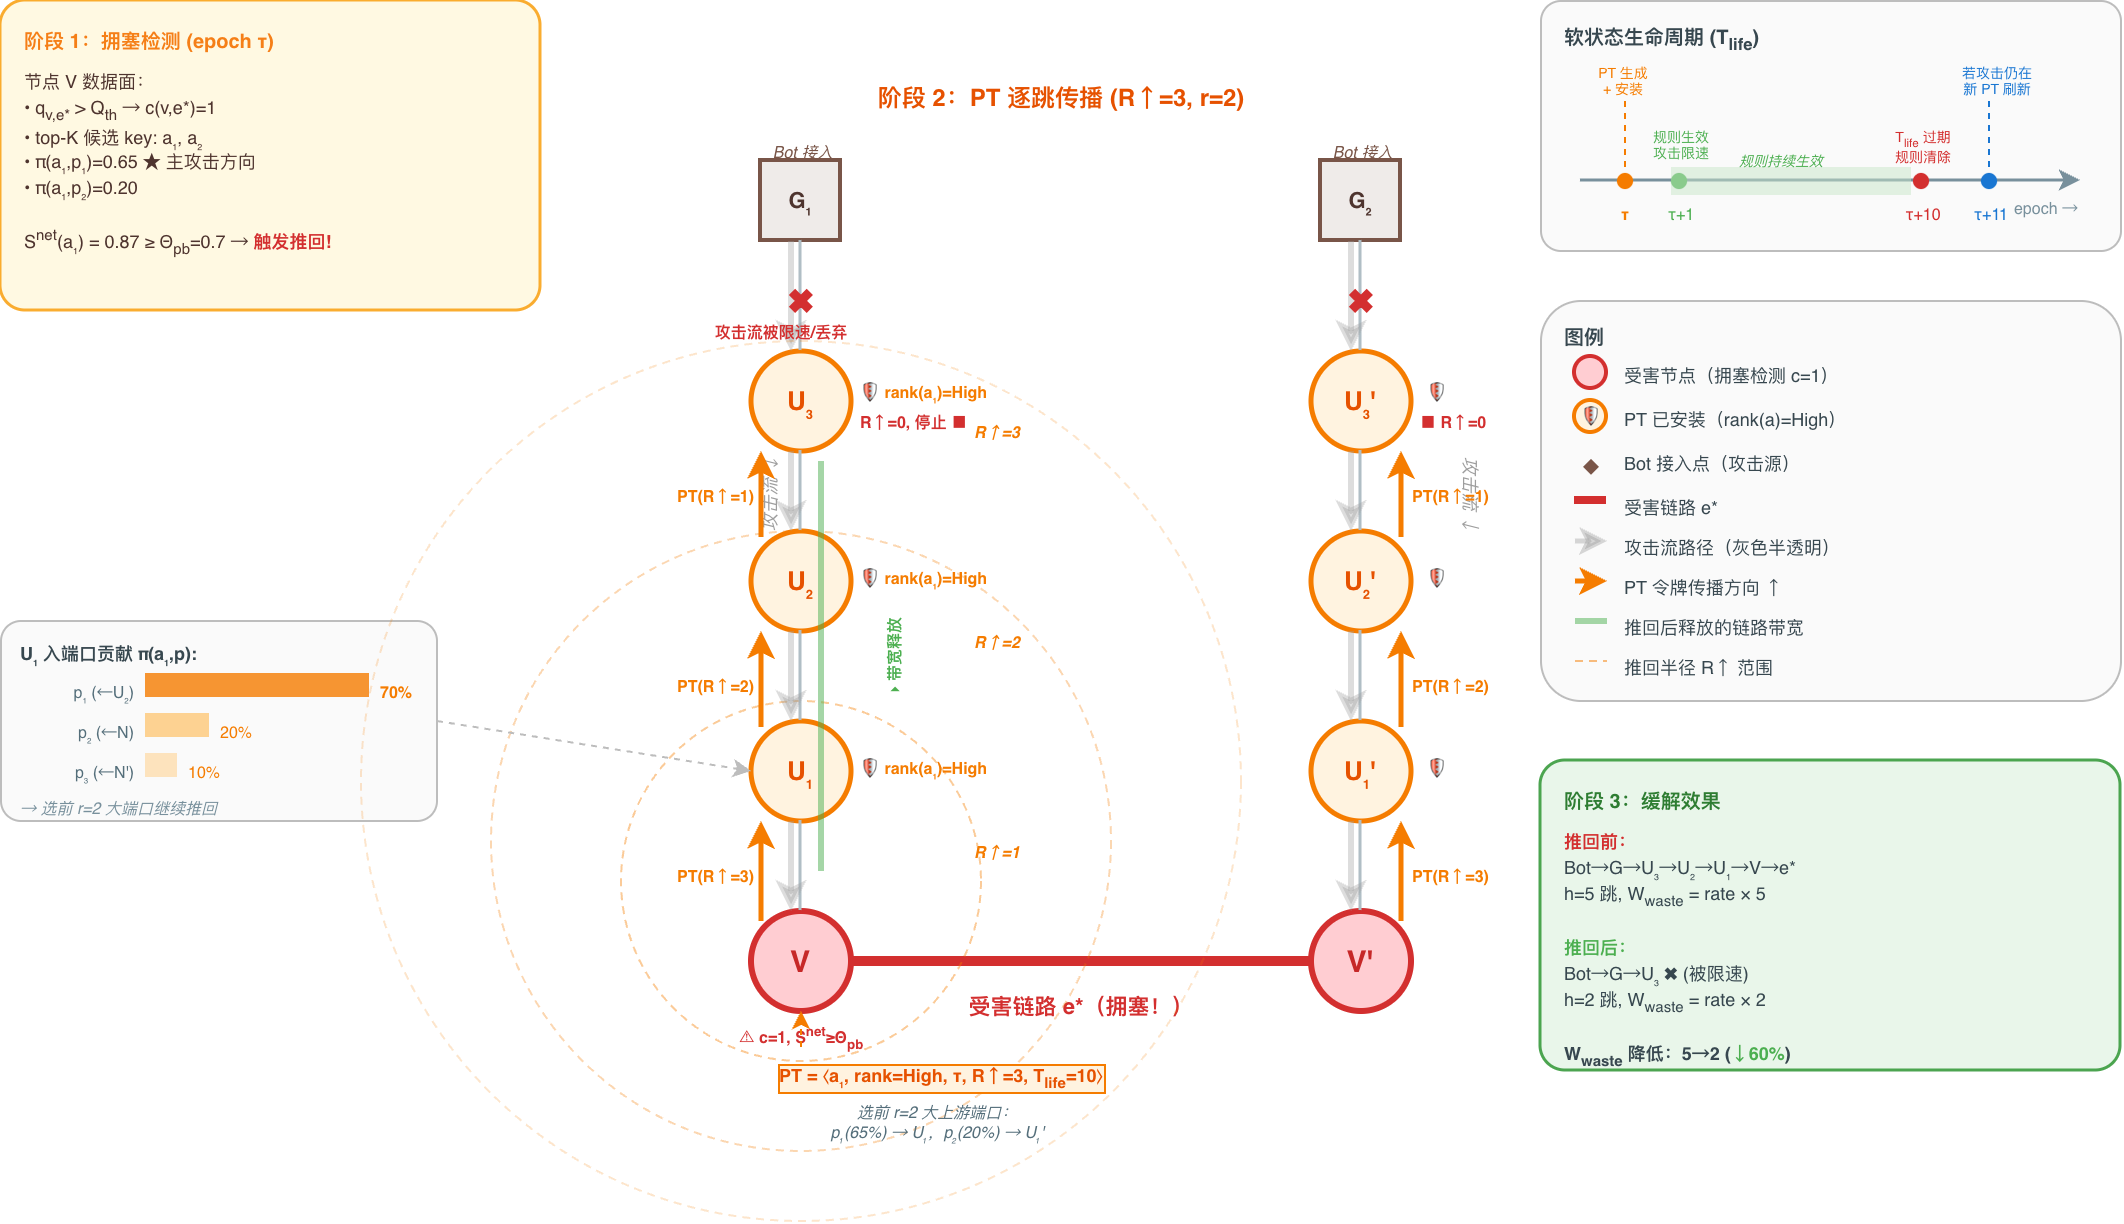
\includegraphics[width=0.93\linewidth]{figs/ch4/fig4_pushback.png}
\caption{\small 逐跳推回缓解传播示意。左上：阶段1——拥塞检测与入端口贡献分布$\pi(a,p)$；中部：阶段2——PT令牌从受害链路$e^*$向上游逐跳扩散（$R_{\uparrow}=3$，$r=2$分支），沿途节点安装软状态缓解规则；右下：阶段3——推回前后的$W_{\text{waste}}$对比（$h$从5跳降至2跳）。右上：软状态生命周期$T_{\text{life}}$时间线。}
\label{fig:ch4_pushback}
\end{figure}

\subsection{信令开销与可实现性分析}
\label{subsec:ch4_overhead}

\subsubsection*{（1）ROI限制下的信令规模上界}
设星座网络的平均度数为$d$（典型LEO ISL结构中$d\approx4$）\citess{icarus}。对任意EG消息，TTL为$R$时，其在最坏情况下可触达的节点数不超过一个$d$叉树的$R$层节点规模：
\begin{equation}
| \text{ROI}(R) | \le 1 + d\cdot \frac{(d-1)^R - 1}{d-2},\quad d>2.
\label{eq:roi_bound}
\end{equation}
当$d=4$时，上界为$| \text{ROI}(R) | \le 2\cdot 3^R -1$。例如$R=4$时，最坏触达规模不超过161个节点，远小于Starlink Shell 1的1584节点总规模\citess{icarus}。因此，TTL本身已经把协同传播限制在受影响的局部区域内，避免全网泛洪。

\subsubsection*{（2）抑制机制下的消息量与带宽开销}
在抑制型扩散中，节点在一个发送窗口内若监听到不少于$k$条等价证据即抑制发送，从而大幅降低重复广播。对\emph{单个协同事件}$(\tau,\texttt{link\_id})$而言，设ROI内有效参与节点数为$N_R$，且每个节点在该事件上每epoch至多发送一次聚合EG消息，则EG消息总数满足：
\begin{equation}
M_{\text{EG}}(\tau,\texttt{link\_id}) \le N_R.
\label{eq:msg_count}
\end{equation}
进一步地，若该事件对应的EG与PT消息大小分别为$L_{\text{EG}}$、$L_{\text{PT}}$字节，PT消息数为$M_{\text{PT}}(\tau,\texttt{link\_id})$，则其单事件控制带宽开销上界为：
\begin{equation}
B_{\text{ctrl}}^{(\tau,\texttt{link\_id})} \le \frac{M_{\text{EG}}(\tau,\texttt{link\_id})\cdot L_{\text{EG}} + M_{\text{PT}}(\tau,\texttt{link\_id})\cdot L_{\text{PT}}}{\Delta}.
\label{eq:ctrl_bw}
\end{equation}
若同一epoch内同时出现多条独立拥塞链路，则总控制开销可写为对所有事件的求和。结合式\eqref{eq:roi_bound}与Starlink ISL 20~Gb/s容量级\citess{icarus}，当$R$取小常数（本章默认$R=4$）时，$B_{\text{ctrl}}$相对ISL带宽占比可控制在远低于$1\%$的量级。实验中我们进一步验证了控制开销与$R,k,\Delta$的敏感性（见第\ref{subsec:ch4_results}节），并观察到抑制机制使得在攻击高峰期也不会出现信令风暴。

\subsubsection*{（3）数据面实现可行性}
实现上，本章遵循数据面负责常数复杂度快路径、控制面负责聚合与决策的分工。数据面新增逻辑主要包括协同消息的轻量 header 解析与 TTL 递减、seen-set 去重（可由 Bloom Filter 近似实现）、key 的入端口贡献统计$\text{bytes}_{v,\tau}(a,p)$，以及 pushback 规则的执行与软状态清理。这些操作都可以由可编程交换机的寄存器阵列与 match-action 表实现\citess{bosshart2013rmt}，每包处理仍保持 O(1) 复杂度，满足线速约束。复杂的聚合评分（式\eqref{eq:net_score}）和抑制决策则交由星上 agent 完成，避免数据面承担过重计算负担。

\section{仿真与分析}
\label{sec:ch4_eval}

\subsection{实验设置}
\label{subsec:ch4_setup}

本章的仿真实验基于自研 Python 仿真框架实现（与\ref{chap:ms_satshield}相同）。该框架集成了星座拓扑构建、最短路计算、epoch 级事件驱动与数据面行为模拟，拓扑构建与路由策略参考 Hypatia 仿真平台\citess{hypatia}的快照路由模型\citess{handley2019delay}。评估采用 Starlink Shell 1 拓扑，该拓扑包含 1584 颗卫星（72 轨道面$\times$22 颗/面），ISL 为典型的 4 链路连接结构，ISL 带宽 20~Gb/s，上下行链路容量为数 Gb/s 量级\citess{icarus}。epoch 长度取$\Delta=1$~s，与卫星拓扑快照更新周期对齐\citess{icarus}。表~\ref{tab:ch4_params}汇总了本章实验使用的主要参数。为贴近真实网络背景流量，本文采用 CAIDA UCSD Anonymized Internet Traces 2018 数据集（OC-192 链路，采集于 Equinix-Chicago 监测点）构造良性流量：原始 trace 按比例缩放至 20~Gb/s ISL 容量级别，并按人口加权的城市对分布模型将源-目的 IP 映射到 LEO 地面终端对，映射参数与\ref{chap:ms_satshield}中的设置一致\citess{satshield}。攻击流量则采用 ICARUS 式 LFA 策略生成，攻击者利用公开轨道与拓扑信息选择 bot 对并计算使目标链路拥塞的流量分配\citess{icarus}；同时，在更强的对手模型下引入低速化、多 decoy、脉冲化和滚动目标等策略，用来检验协同机制对碎片化证据的聚合能力。

为避免实验设置中声明的指标多于正文实际汇报的指标，本章只报告与后续图表直接对应的四类结果：路径积分无效带宽占用成本$W_{\text{waste}}$（单位 Mb/s$\cdot$hop，对应式\eqref{eq:waste_bw}）；攻击期间的良性吞吐，以及两类响应时延，本地检测生效时延$T_{\text{det}}=t_{\text{first-local-rule}}-t_{\text{attack-start}}$和 pushback 生效时延$T_{\text{pb}}=t_{\text{first-pushback-rule}}-t_{\text{attack-start}}$；检测质量，即攻击相关 key 识别的 Precision、Recall 和 F1（定义同\ref{chap:ms_satshield}式( \ref{eq:f1_def} )）；以及协同开销，即 EG/PT 消息数与字节开销。除非特别说明，下文提到的吞吐都指攻击持续阶段的 epoch 平均值，不包含 warmup 与恢复段。

\begin{table}[t]
\centering
\caption{第四章实验主要参数设置}
\label{tab:ch4_params}
\begin{tabular}{l|l|l}
\hline
参数 & 含义 & 取值 \\
\hline
$\Delta$ & epoch长度 & 1~s \\
$I$ & 抑制扩散时隙 & $\Delta/4 = 0.25$~s \\
$R$ & ROI半径（EG TTL） & 4跳 \\
$R_{\uparrow}$ & 推回半径（PT跳数） & 3跳 \\
$k$ & 抑制参数 & 3 \\
$n$ & EG携带的top-$n$ key数 & 10（默认）；图~\ref{fig:ch4_ctrl_overhead}(b)按保守$n=100$计费 \\
$r$ & 推回上游分支数 & $\min(2,d-1)=2$ \\
$\theta_\Omega$ & 相关性门限 & 0.3 \\
$Q_{\text{th}},D_{\text{th}}$ & 拥塞告警阈值 & 继承第\ref{chap:ms_satshield}章部署配置（本章不单独调参） \\
$\Theta_{\text{pb}}$ & 推回判定阈值 & 0.7 \\
$\lambda$ & 拥塞权重放大因子 & 1.0 \\
$\mu$ & 距离衰减因子 & 0.5 \\
$T_{\text{life}}$ & PT软状态生存期 & 10 epoch \\
\hline
\end{tabular}
\end{table}

\begin{table}[t]
\centering
\caption{量化对比基线设置（第四章正文结果）}
\label{tab:ch4_baselines}
\begin{tabular}{l|l}
\hline
方案 & 说明 \\
\hline
NoDefense & 无防御，FIFO/ECMP默认转发 \\
SatShield & 单星top-$k$过滤+队列调度缓解\citess{satshield} \\
MS-SatShield & \ref{chap:ms_satshield}多签名增强，但无协同/无pushback \\
\textsc{CoopSatShield} & 本章方案：抑制型扩散协同+逐跳pushback \\
\hline
\end{tabular}
\end{table}

表~\ref{tab:ch4_baselines}中的四种方案构成了本章正文图表的量化比较范围。至于 LinkScope、Woodpecker、RADAR、Ripple 与 Mew 等典型地面 LFA 防御机制\citess{linkscope,woodpecker,radar,ripple,mew}，本文仍将其作为相关工作与设计参照。它们分别代表主动测量、集中式流量工程、相关性检测和可编程数据面分布式防御等不同技术路线，但由于这些方案依赖的控制闭环、硬件资源或拓扑稳定性假设与 LEO 场景差异明显，本章尚未在统一的 LEO 仿真口径下完成等价复现，因此不把它们写成正文中的数值基线，也不据此宣称实验优势。若后续补齐统一实现，更合适的呈现方式应是一张代表场景下的指标汇总表，而不是继续堆叠多条长曲线。

\subsection{结果与分析}
\label{subsec:ch4_results}

\subsubsection*{（1）推回缓解带来的网络级收益}
图~\ref{fig:ch4_waste_reduction}以分组柱状图展示了在不同碎片化程度$M\in\{1,10,100,1000\}$下，各方案对路径积分无效带宽占用成本$W_{\text{waste}}$的影响。实验结果可以分为三种情形来看。

当$M\leq10$时，SatShield与MS-SatShield表现接近，均可将$W_{\text{waste}}$降至 NoDefense 的$7.2\%$（$M=1$）和$19.8\%$（$M=10$）。这是因为此时攻击 key 的聚合速率远高于良性长尾，rate-only 已能稳定检出，多签名不会带来额外增益。CoopSatShield 则通过推回把丢弃位置继续前移到上游$R_{\uparrow}=3$跳附近，使$W_{\text{waste}}$在$M=1$时进一步降到$3.0\%$。这里的收益主要来自 pushback 缩短攻击流实际承载路径，而不是协同证据聚合；在$M=1$时，单节点已经足以检出唯一的攻击 key。这说明即使不存在明显碎片化，pushback 本身也具有独立的带宽节约价值。

当$M=100$时，SatShield 的 rate-only 检测已经基本失效（F1$=0.017$），$W_{\text{waste}}=248{,}995$~Mb/s$\cdot$hop，与 NoDefense 的$251{,}005$只差$0.8\%$，几乎等同于无防御。这一结果与\ref{chap:ms_satshield}图~\ref{fig:ch3_fig2_f1}(b)中的分离段分析一致，因为在$M=100$时速率特征已经落入良性长尾。MS-SatShield 依靠 FO/FI 特征仍能保持有效检测（F1$=0.909$），使$W_{\text{waste}}$降至 NoDefense 的$17.1\%$；CoopSatShield 再通过推回把这一比例进一步压低到$11.0\%$，相较 MS-SatShield 额外释放了$6.1$个百分点的链路带宽。

当$M=1000$时，攻击 key 大量脱离 top-$K$候选集（TopK~Recall$\approx0.30$），所有方案的$W_{\text{waste}}$都明显上升。MS-SatShield 与 CoopSatShield 仍然优于 SatShield，分别占 NoDefense 的$72.5\%$和$70.8\%$，但改善幅度已经有限，这反映的正是\ref{chap:ms_satshield}中指出的候选集覆盖率瓶颈。

这些结果与式\eqref{eq:waste_bw_approx}描述的推回收益机理是一致的，即推回把攻击流的平均承载跳数$\bar h$从完整路径长度压缩到$R_{\uparrow}$跳量级。同时，不同$M$值下的渐进退化设定也延续了\ref{chap:ms_satshield}中的分析路径：先是 rate-only 仍然有效，再到需要多签名补偿，最后进入候选集覆盖率受限的区间。

\begin{figure}[!htb]
\centering
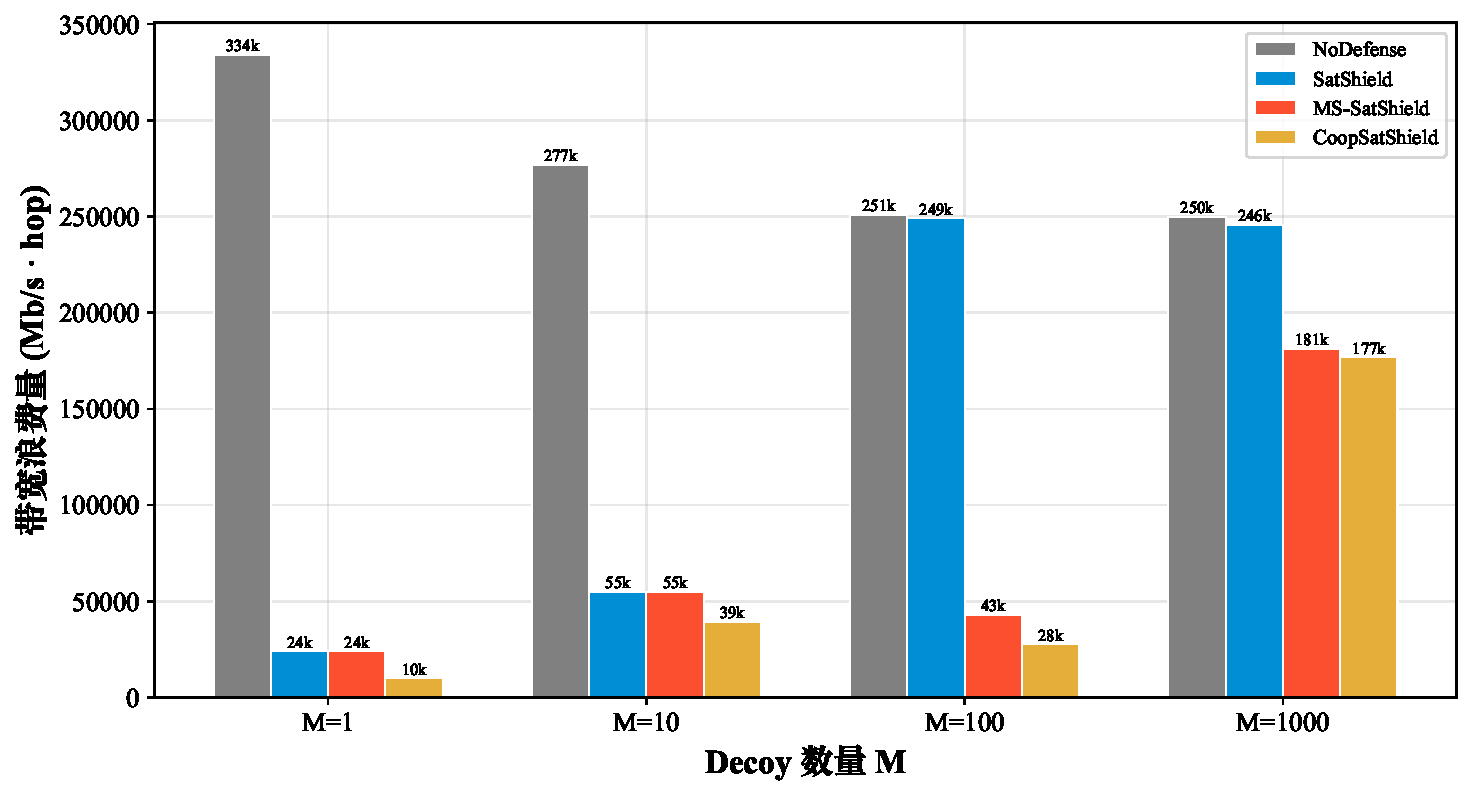
\includegraphics[width=0.92\linewidth]{figs/ch4/fig4_waste.pdf}
\caption{不同碎片化程度$M$下的无效带宽占用$W_{\text{waste}}$对比。四组分组柱状图分别对应$M=1,10,100,1000$，每组包含NoDefense（灰）、SatShield（蓝）、MS-SatShield（红）、CoopSatShield（金）四种方案，柱顶标注具体数值。}
\label{fig:ch4_waste_reduction}
\end{figure}

\subsubsection*{（2）良性吞吐与反应时间}
图~\ref{fig:ch4_throughput}给出了$M=100$攻击场景下良性吞吐随时间（epoch）变化的全过程。实验将攻击窗口设置为 epoch~30 至 epoch~120（共 90 个 epoch），图中粉色背景标出攻击持续阶段，竖虚线分别对应攻击开始、首次检测和推回生效三个时刻。按上一节的定义，本地检测生效时延为$T_{\text{det}}=1$~epoch，pushback 生效时延为$T_{\text{pb}}=2$~epoch。

\textbf{攻击前}（epoch~0$\sim$29），所有方案的良性吞吐都稳定在 1.0 附近，符合网络正常运行状态。

\textbf{攻击触发与检测延迟}（epoch~30）：由于检测算法至少需要 1 个 epoch 的统计积累，攻击开始后的第一个 epoch 内所有方案都无法检出攻击流，良性吞吐统一跌至 NoDefense 水平$\approx0.71$。这一短暂下探反映的是在网检测的内在时滞，对所有基线都成立。

\textbf{首次检测生效}（epoch~31）：SatShield 的 rate-only 检测在$M=100$下完全失效（F1$=0.017$），因此吞吐仍维持在 NoDefense 水平。MS-SatShield 依靠多签名检测能力（F1$=0.909$），通过高优先级队列保留机制（80\% 带宽保留）将攻击期间的良性吞吐恢复到$0.886$，相对 NoDefense 提升了$17.5$个百分点。CoopSatShield 在这一时刻暂时与 MS-SatShield 处于同一水平，因为检测已经生效，但推回尚未传播完成。

\textbf{推回生效}（epoch~32+）：当 gossip 消息完成 ROI 内扩散后，CoopSatShield 的 pushback 规则开始在上游节点生效，约$86\%$的已检测攻击流在上游被直接丢弃，中间链路带宽因此得到释放。稳态下，CoopSatShield 的吞吐恢复至$0.959$，相较 MS-SatShield 进一步提升了$7.3$个百分点。由于推回覆盖率并未达到$100\%$，仍有约$14\%$的攻击流沿非推回路径到达目标链路，因此稳态吞吐停留在$0.959$而不是理想的$1.0$，这体现了分布式推回在工程实现上的实际边界。

\textbf{攻击结束}（epoch~120后）：所有方案的吞吐都迅速恢复到$1.0$附近。整体来看，CoopSatShield 的吞吐恢复表现为两个连续阶段：先由检测触发的队列调度提供基础保护（$+17.5$~pp），再由推回带来的上游丢弃继续提供增量收益（$+7.3$~pp），最终使良性吞吐在攻击期间稳定维持在约$0.96$。

\begin{figure}[!htb]
\centering
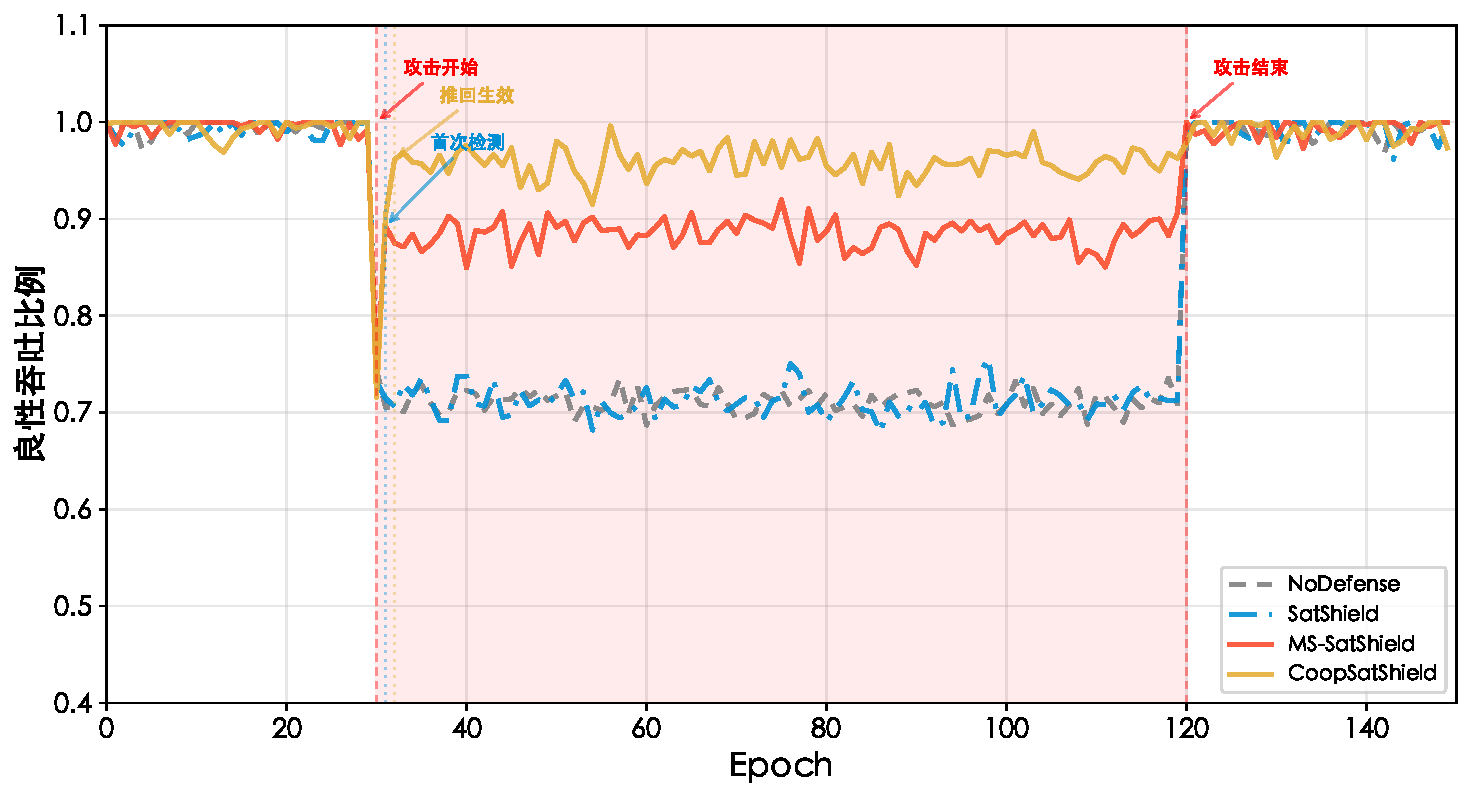
\includegraphics[width=0.92\linewidth]{figs/ch4/fig4_throughput.pdf}
\caption{良性吞吐随时间变化（$M=100$）。粉色背景标注攻击持续阶段（epoch~30$\sim$120），竖虚线分别对应攻击开始、首次检测与推回生效三个时刻。CoopSatShield经历两步递升：检测恢复至0.89，推回进一步至0.96。}
\label{fig:ch4_throughput}
\end{figure}

\subsubsection*{（3）协同开销与无信令风暴验证}
本章最关心的工程风险之一，是大规模网络中的信令风暴。图~\ref{fig:ch4_ctrl_overhead}用$1\times3$子图展示了协同开销和抑制机制的效果。

子图~(a)比较了有抑制（$k=3$）和无抑制两种情况下，EG 消息数随 ROI 半径$R$的变化。无抑制时，EG 消息数从$R=1$的 45 条增长到$R=6$的 765 条，接近超线性增长；加入抑制后，同一区间只从 45 条增长到 347 条。在$R=4$时，抑制机制把消息数从 369 条压低到 203 条，减少了$45\%$。PT 消息数则稳定在 44 条，因为它只沿推回路径单向传播，不受$R$影响。图中的浅红色填充区域直观展示了抑制带来的收益。

子图~(b)进一步将消息数换算为控制带宽（KB/epoch），并用右侧$y$轴给出其占 ISL 容量（20~Gb/s）的百分比。这里的字节统计采用了更保守的 EG 载荷配置$n=100$，并将 EG 与 PT 消息一并计入，因此 104~KB/epoch 应理解为压力条件下的上界估计，而不是默认$n=10$配置下的运行时均值。在推荐配置$R=4$时，该口径下的控制带宽仅占 ISL 容量的$0.004\%$；即使在$R=6$的最大测试半径下，占比也不超过$0.008\%$。这说明协同开销本身很低，也与式\eqref{eq:roi_bound}和式\eqref{eq:ctrl_bw}的理论分析一致。

子图~(c)展示了抑制参数$k$对 EG 消息数与抑制率的影响。$k=1$时抑制率高达$80\%$，但消息只有 9 条，覆盖明显不足；$k=10$时抑制率降到$0\%$，基本等同于无抑制。本文推荐的$k=3$（图中红色标注）在覆盖与开销之间取得了较好的平衡，此时抑制率为$30\%$，消息数为 203 条。基于当前结果，可以把$k=3$视为工程上可工作的默认配置；它对检测质量的影响仍需在后续补充实验中与$k=10$等配置进一步比较。

\begin{figure}[!htb]
\centering

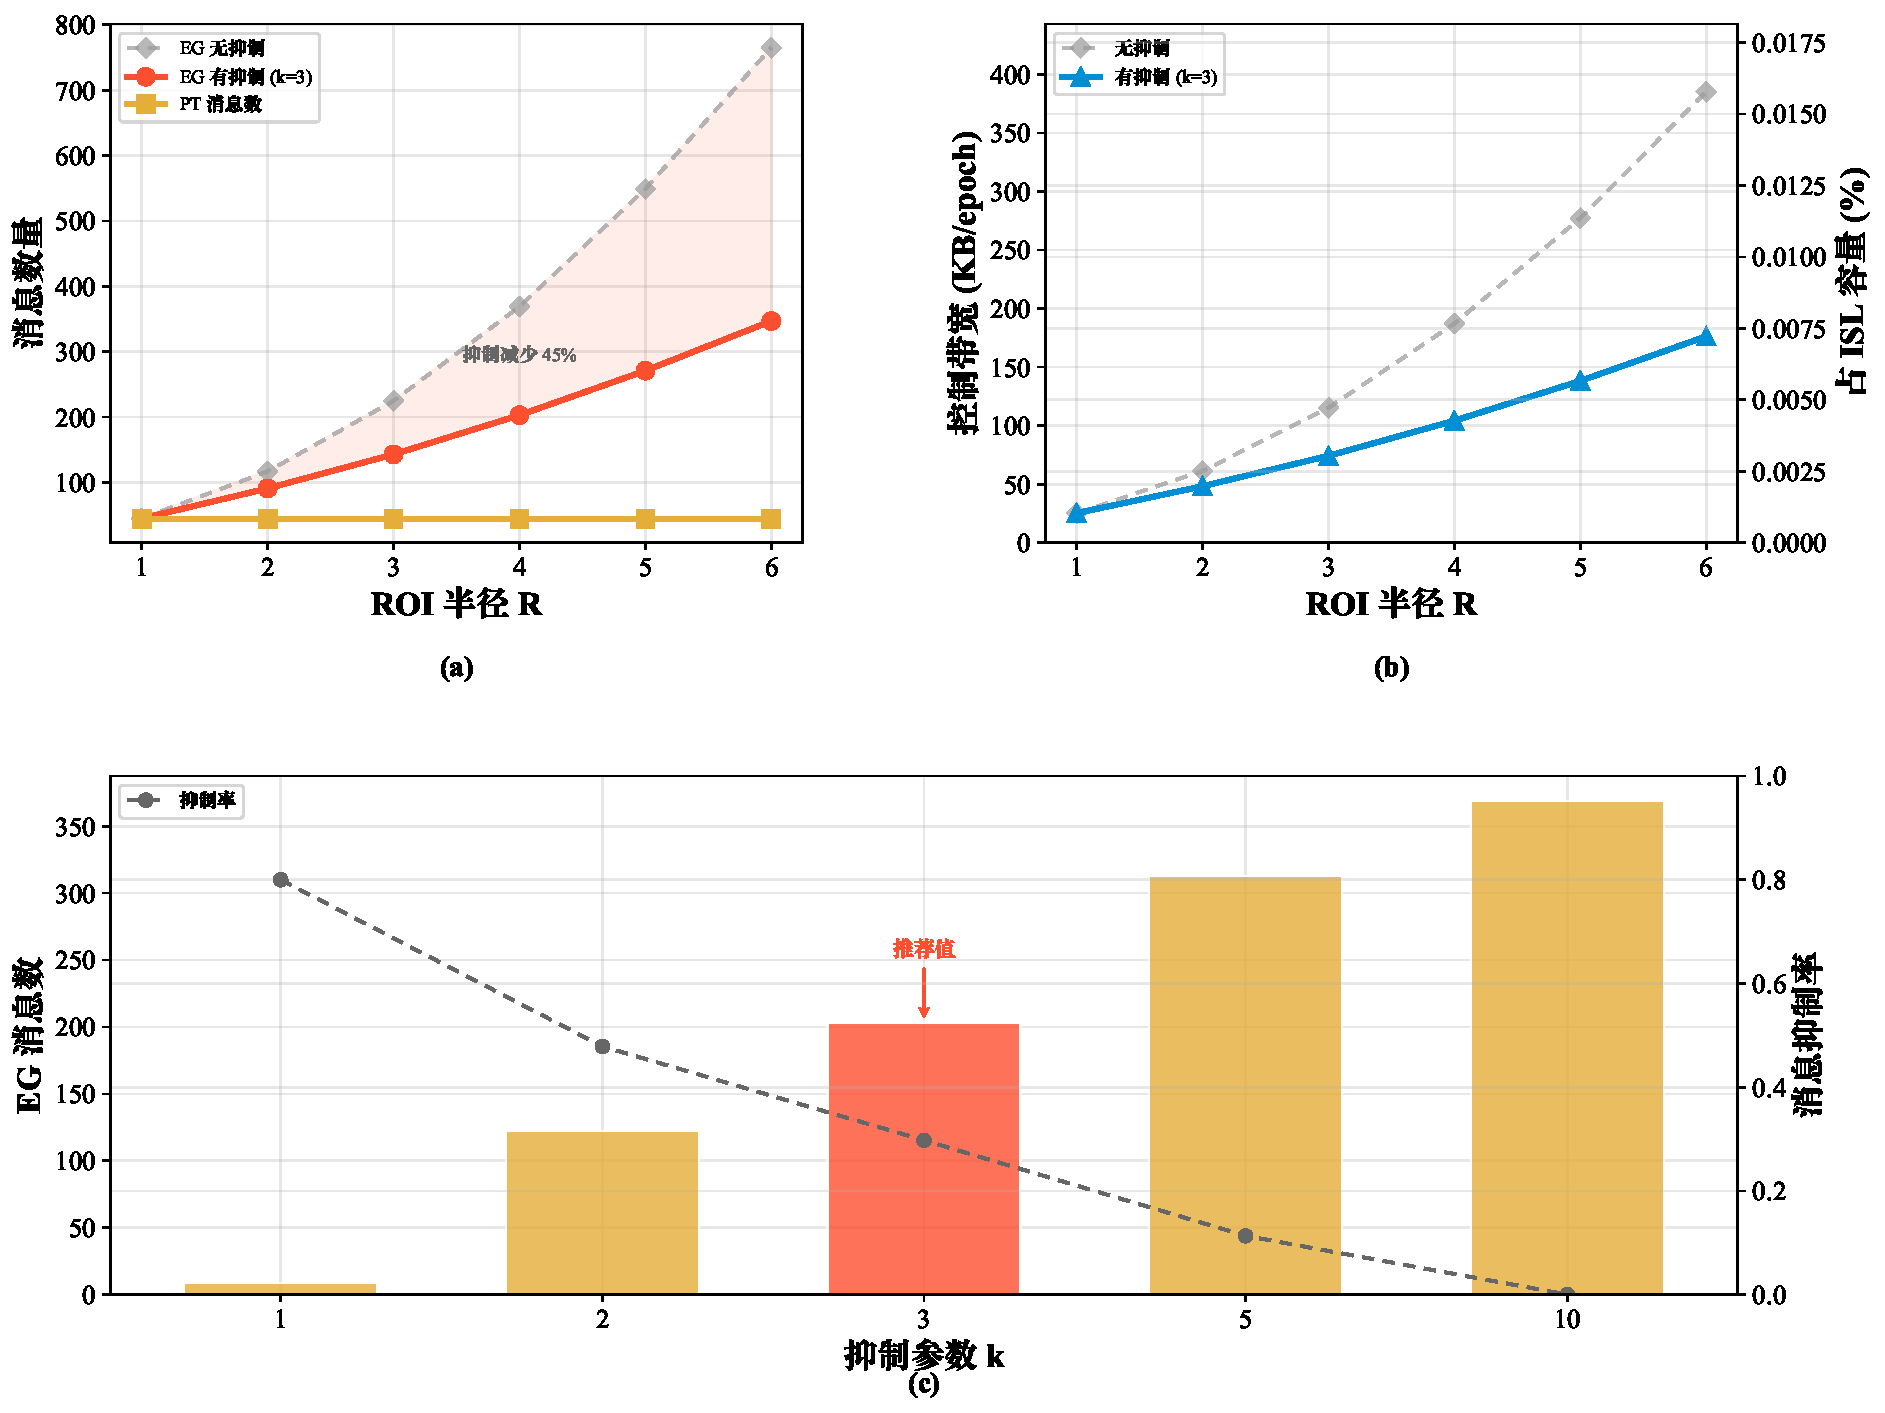
\includegraphics[width=0.92\linewidth]{figs/ch4/fig4_overhead.pdf}
\caption{协同控制开销与抑制机制效果。(a)EG消息数随$R$变化：灰色虚线为无抑制基线，红色实线为有抑制（$k=3$），填充区域为抑制收益；(b)控制带宽随$R$变化，按保守的$n=100$口径统计EG载荷并计入PT总字节，右轴标注占ISL容量百分比（$R=4$时仅$0.004\%$）；(c)抑制参数$k$的影响，$k=3$为工程默认值。}
\label{fig:ch4_ctrl_overhead}
\end{figure}

\subsubsection*{（4）对碎片化攻击证据的鲁棒性}
图~\ref{fig:ch4_robustness}用$2\times2$子图评估了各方案在碎片化攻击（$M\in\{1,5,10,50,100,500,1000\}$）下的表现。四个子图分别给出检测效果（F1 与 Recall）、检测精度（Precision）、良性吞吐恢复以及无效带宽占用。

\textbf{F1 的倒 U 型变化}（子图(a)）：MS-SatShield 与 CoopSatShield 的 F1 随$M$呈现倒 U 型，而不是简单的单调递减，这一变化大致可以分成三段。

当$M\leq10$时，所有方案的 Recall 都保持在$1.0$（虚线所示），说明攻击 key 已被完整捕获；但 F1 仍然偏低，例如$M=1$时约为$0.09$。原因并不在于漏检，而在于存在约 19 个良性重流 key 被持续误判为可疑，这些 key 的聚合速率为$474\sim606$~Mb/s，超过$\tau\cdot\text{rate}_{p99}=242.5$~Mb/s。由子图(b)可见，$M=1$时 Precision 只有$0.05$（TP$=1$，FP$\approx19$），因此 F1 偏低主要是 Precision 不足造成的。这里需要强调，F1 较低并不意味着检测无效：在$M=1$时，唯一的攻击 key（聚合速率$10{,}024$~Mb/s）仍被正确识别，子图(c)也表明 SatShield 与 MS-SatShield 的吞吐都恢复到了$0.886$，CoopSatShield 通过推回则进一步恢复到$1.000$。

当$M=50\sim100$时，攻击 key 数量已经明显多于误报数，FO/FI 特征开始有效地区分攻击流量与良性流量。$M=100$时，MS-SatShield 的 Precision 升至$0.833$，Recall 仍保持$1.0$，F1 达到峰值$0.909$。同一区间内，SatShield 已经完全失效，$M=50$时 F1 仅为$0.057$，$M=100$时进一步降到$0.017$，因为此时攻击 per-key 速率已经接近良性$p_{99}$，rate-only 无法完成区分。这一结果与\ref{chap:ms_satshield}图~\ref{fig:ch3_fig2_f1}(b)中的分离段分析保持一致。

当$M\geq500$时，攻击 key 的单 key 速率降至$20\sim35$~Mb/s，大量 key 脱离 top-$K$候选集（TopK~Recall$\approx0.30$）。MS-SatShield 的 Precision 反而提高到$0.936\sim1.000$，因为被筛入候选集的攻击 key 几乎都能被正确识别，但 Recall 只有$0.30$，最终使 F1 降至$0.445\sim0.466$。

\textbf{CoopSatShield 与 MS-SatShield 的 F1 完全一致}（子图(a)中两条 F1 实线重合）。原因在于二者共享同一检测流水线，即同一个多签名评分器。在当前实验采用的 bot 均匀分布场景下，各节点的本地 top-$K$命中率已经足够高，协同证据聚合不会改变单节点的检测输出。因此，本章协同机制的价值主要体现在缓解层面，而不是检测层面。gossip 负责跨节点共享攻击信息，pushback 则据此把缓解动作从受害链路前推到更上游的入口，这正对应了引言中提出的上游带宽浪费问题。子图(c)显示，在低到中等碎片化范围内，CoopSatShield 的良性吞吐明显高于 MS-SatShield。若统一采用与图~\ref{fig:ch4_throughput}一致的攻击期间稳态平均吞吐口径，则$M\leq 50$时其恢复值接近$1.000$，$M=100$时仍为$0.959$，显著高于 MS-SatShield 的$0.886$；子图(d)则显示，CoopSatShield 的$W_{\text{waste}}$在各个$M$值下都保持最低，这也与图~\ref{fig:ch4_waste_reduction}中的渐进退化分析一致。当$M\geq500$时，所有方案的吞吐都开始退化，CoopSatShield 也下降到$0.80$，反映出候选集覆盖率瓶颈最终会传导到缓解层面。需要补充说明的是，在 bot 分布极不均匀的特定场景下，例如攻击流量集中经过少数中继节点、而这些节点的本地候选集又无法完全覆盖时，协同聚合仍然可能提高检测 Recall；但在本章采用的均匀 bot 分布假设下，这种效果没有显现。

% TODO: 这里的图口径和上一章的图口径不一致，需要统一
% \noindent\textbf{图口径说明。} 若后续重绘图~\ref{fig:ch4_robustness}(c)，建议将$M=100$点调整为与图~\ref{fig:ch4_throughput}一致的稳态平均口径；若沿用当前导出脚本，则应至少在图注中显式注明其统计定义是“恢复峰值”还是“攻击期均值”。

\begin{figure}[!htb]
\centering
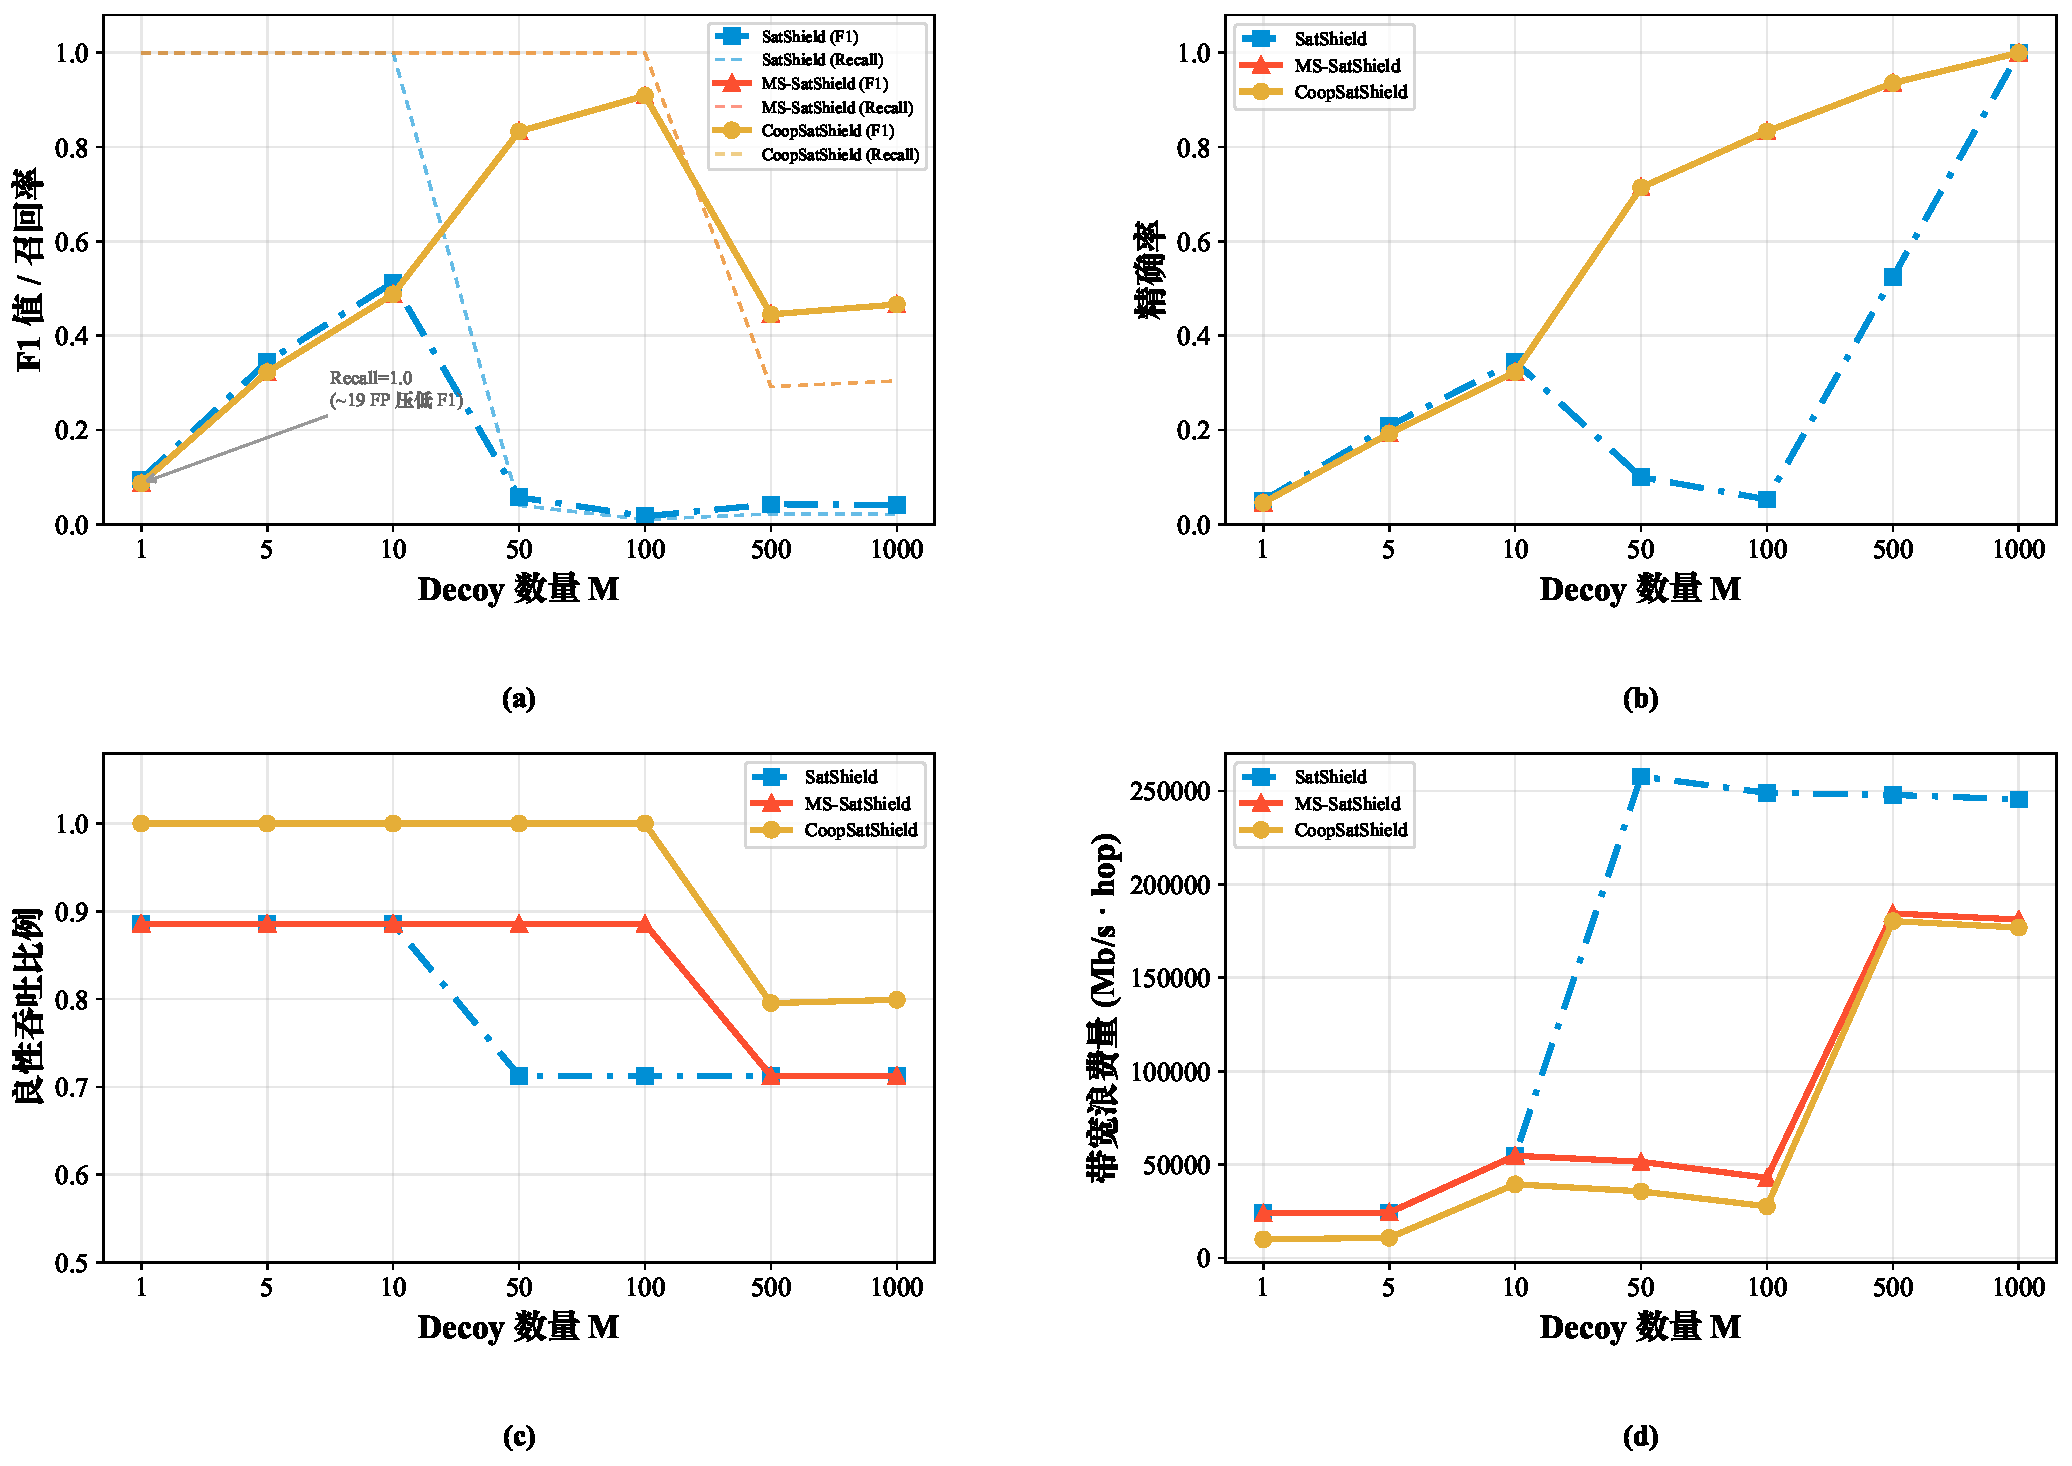
\includegraphics[width=0.92\linewidth]{figs/ch4/fig4_robustness.pdf}
\caption{碎片化攻击下的鲁棒性（$2\times2$子图）。(a)F1（实线）与Recall（虚线）随$M$变化，注意$M\leq10$时F1低是Precision不足所致，Recall始终为1.0；(b)Precision随$M$变化；(c)良性吞吐恢复；(d)无效带宽$W_{\text{waste}}$。}
\label{fig:ch4_robustness}
\end{figure}

\subsection{适用边界与讨论}
\label{subsec:ch4_discussion}

\noindent\textbf{量化比较范围。} 本章正文中的数值比较严格限定在 NoDefense、SatShield、MS-SatShield 与 CoopSatShield 四类星载方案之内。LinkScope、Woodpecker、RADAR、Ripple 与 Mew 等地面 LFA 防御机制仍然有参考价值，但在统一的 LEO 实现完成之前，它们更适合作为设计假设和控制闭环差异的讨论对象，而不适合直接写入本章实验结论。

\noindent\textbf{协同聚合的作用层次。} 在当前均匀 bot 分布设定下，协同聚合评分$S^{\text{net}}$并未改变检测 F1，因此本章能够支持的主要结论是：加权聚合有助于稳定 pushback 触发，但没有表现出显著提高检测能力的作用。若后续需要进一步说明式\eqref{eq:net_score}与式\eqref{eq:weight}相对于简单 avg 或 max 规则的必要性，最直接的办法是补充聚合规则消融以及$\Theta_{\text{pb}},\lambda,\mu$的敏感性实验。

\noindent\textbf{推回覆盖率与候选集瓶颈。} CoopSatShield 在$M=100$时仍只能将稳态良性吞吐恢复到$0.959$，说明近似反向路径推回与局部 ROI 覆盖仍然受制于拓扑分叉和路径不确定性；当$M\ge 500$时，一级候选集覆盖率下降又会进一步把检测瓶颈传导到缓解层面。就本章的证据而言，可以较明确地说明推回能够前移缓解位置并显著降低网络内部成本，但还不能说明它在任意碎片化强度下都能近乎完全消除攻击影响。

\section{本章小结}
\label{sec:ch4_summary}

本章面向大规模低轨卫星网络中的链路洪泛攻击，将研究范围从单星本地闭环防御进一步扩展到多星协同在网计算与推回缓解。针对 LEO 网络中控制环延迟高、拓扑变化快、攻击自适应速度快等约束\citess{satshield,icarus}，本文提出\textsc{CoopSatShield}：在\ref{chap:ms_satshield}的本地多签名检测基础上，将检测输出组织为可协同处理的证据单元；设计抑制型邻居扩散协议，通过事件驱动、ROI 限制和冗余抑制来控制大规模网络中的信令扩散；再结合逐跳 pushback 机制，利用入端口贡献分布实现不依赖全局逆路由的推回缓解，把攻击抑制位置前移到上游入口，从而降低网络内部无效带宽占用并提升良性吞吐保护。

实验结果表明，CoopSatShield 在$M=100$时可将路径积分无效带宽占用成本$W_{\text{waste}}$降至 NoDefense 的$11.0\%$，相比 MS-SatShield（$17.1\%$）再降低$6.1$个百分点；在良性吞吐方面，攻击期间的稳态吞吐维持在$0.959$，相较 MS-SatShield（$0.886$）提升$7.3$个百分点，本地检测与 pushback 的生效时延分别为$T_{\text{det}}=1$~epoch和$T_{\text{pb}}=2$~epoch；在协同开销方面，推荐配置$R=4,k=3$下，按保守$n=100$口径统计的控制带宽仅占 ISL 容量的$0.004\%$，抑制机制还使 EG 消息数比无抑制基线减少$45\%$，没有出现信令风暴；在碎片化攻击场景下，$M=100$时 F1 达到峰值$0.909$，低至中等碎片化范围内良性吞吐接近$1.000$，即使在$M=100$时也仍保持$0.959$。这些结果把全文关于大规模低轨卫星在网计算的研究，从单节点处理自然推进到了多节点协同处理。

\noindent\textbf{局限性与未来方向。} 本章仍有几方面局限。首先，在本章采用的均匀 bot 分布假设下，协同聚合评分$S^{\text{net}}$并未改变单节点检测输出，因此协同的主要收益仍停留在缓解层面，也就是 pushback；在 bot 分布极不均匀或攻击流量集中经过少数中继节点的场景下，协同聚合可能提高检测 Recall，但这一点还需要专门验证。其次，候选集覆盖率仍是主要瓶颈。$M\geq500$时，大量攻击 key 的单 key 速率低于 top-$K$门限而脱离候选集，导致所有方案的 F1 与吞吐保护都开始退化。如何在候选集规模与数据面资源消耗之间找到更合适的平衡，仍有待进一步研究。最后，本章默认所有邻居节点均可信，没有考虑恶意节点注入虚假 EG/PT 消息的情况。针对这类拜占庭攻击，后续可以引入轻量级签名或声誉机制来验证消息；此外，跨轨道面协同以及与 SDN 控制面的混合架构对接，也值得继续展开。


\chapter{总结与展望}
\label{chap:conclusion}

\section{全文总结}

大规模低轨（LEO）卫星巨型星座凭借其低时延、广覆盖的通信能力，正在成为下一代天地一体化信息网络的战略基础设施。然而，星间链路（ISL）带宽有限、卫星轨道参数完全公开的特性，使 LEO 星座网络面临链路洪泛攻击（LFA）的严峻威胁。本文围绕"如何在星载可编程数据面的严苛 SWaP 约束下，构建低时延、低资源消耗且能有效对抗 LFA 退化策略的在网安全防御体系"这一核心问题，以在网计算为技术路线，开展了从单节点多签名检测到多节点协同推回缓解的系统性研究。全文的主要研究成果总结如下。

（1）\textbf{面向 LEO 网络的多签名在网检测与队列缓解方法（MS-SatShield）。} 本文在第三章中针对单节点在 P4 数据面上进行 LFA 检测时面临的特征退化困境，提出了一种多签名在网检测与队列缓解方法。该方法的核心创新在于设计了级联式两级检测流水线架构：第一级采用“Count-Min Sketch 频率估计 + 固定容量候选缓存”的 sketch-based 候选生成机制，以固定内存维护全局近似频次并显式恢复候选 key 集合；第二级在候选集上部署双缓冲位图结构，在线提取扇入度（FI）、扇出度（FO）和历史持续性（Persist）等多维结构特征签名。通过“仅对候选集合维护 FI/FO”的设计，该方法将 distinct 统计的状态成本严格控制在 $O(K \cdot m)$ 范围内（默认 $K=1000$, $m=256$, 数据面总状态约 200~KB），天然契合星载平台的 SWaP 约束。实验结果验证了该方法的有效性：在多 decoy 分摊退化设定下（$M=100$），仅靠聚合速率的基线方案 F1 降至 0.017，而引入 FI/FO 后的 MS-SatShield F1 恢复至 0.908，FI/FO 特征提供了核心检测增益；在脉冲式 on-off 攻击下，持续性特征通过加性奖励与候选集扩展机制将 Recall 提升至 0.999，良性吞吐恢复至 0.885；消融实验表明了 $K \approx 1000$、$m = 256$、$\Delta = 1.0$~s 在检测精度与资源开销之间经验上较优的参数折中。

（2）\textbf{基于抑制型扩散的多星协同在网计算与推回缓解方法（CoopSatShield）。} 本文在第四章中针对单星检测视野的局限性与"被动就地丢弃"模式的不足，提出了一种多星协同在网计算与逐跳推回缓解方法。该方法包含两个核心组件：抑制型流言传播协议（Suppressed Gossip Protocol）和逐跳推回缓解机制（Hop-by-hop Pushback）。前者通过事件驱动、区域限制（ROI, $R=4$ 跳）与基于 Trickle 思想的冗余抑制三重约束，在严格限制信令开销的前提下实现局部区域内多颗卫星之间的攻击证据快速交叉验证与聚合；后者利用入端口贡献分布实现无需全局逆路由的推回令牌传播，将攻击抑制点从受害链路前推至上游入口，有效减少攻击流在网络中的无效传输。实验结果表明了该方法的显著优势：在 $M=100$ 退化下，CoopSatShield 将路径积分意义下的无效带宽占用成本（$W_{\text{waste}}$）降至无防御方案的 11.0\%，相比 MS-SatShield 进一步降低 6.1 个百分点；攻击期间良性吞吐稳态维持在 $0.959$，相比 MS-SatShield 提升 7.3 个百分点；推荐配置 $R=4, k=3$ 下，按保守 $n=100$ 口径统计的控制带宽仅占 ISL 容量的 0.004\%，抑制机制使 EG 消息数比无抑制基线减少 45\%，证实了协同通信不会引发信令风暴。

上述两项研究成果共同构成了面向大规模 LEO 卫星网络的在网计算安全防御体系，实现了从"单节点在网计算"到"多节点协同在网计算"的完整技术链条。在理论层面，本文揭示了 LFA 攻击退化策略与多维特征签名之间的对偶约束关系——攻击者无法在压缩速率特征的同时压缩 FI/FO 特征，为多签名检测提供了理论基础。在方法层面，本文提出了级联式两级检测架构和抑制型邻居扩散协同框架，将安全检测与缓解逻辑完整下沉至星载可编程数据面，规避了星地控制环路的时延瓶颈。在系统层面，数据面总状态开销控制在约 200~KB，控制信令带宽不超过 ISL 容量的 0.004\%，满足了星载环境的资源约束。

\section{未来展望}

本文围绕低轨卫星网络中的链路洪泛攻击防御开展了研究，并在单星检测、多星协同和逐跳推回等方面取得了较好的实验结果。随着星座能力持续提升，未来的研究还需要考虑新型业务载荷和更复杂网络组织形态带来的新需求。基于这一判断，后续工作可重点从以下两个方向继续展开。

（1）\textbf{面向多业务与在轨计算载荷的防御扩展。} 未来低轨卫星网络将不再只是单纯的宽带转发网络，而会同时承载公众接入、企业专网、政府业务以及在轨 AI 处理和空间侧算力协同等任务\citess{starlink_direct_to_cell_2026, amazon_leo_enterprise_2025, xinhua_space_computing_2026}。这意味着网络中的关键对象将从传统链路和队列进一步扩展到模型分发路径、在轨推理结果、跨星算力调度和业务切片保障等新型载荷。相应地，后续研究可在本文框架基础上进一步考虑面向多类业务与计算任务的分级检测、差异化缓解与联合保障机制，使在网防御能够同时适应通信业务和计算载荷并存的运行环境。

（2）\textbf{面向跨区域与异构星座场景的协同扩展。} 本文第四章主要围绕单一星座内的局部协同与逐跳推回展开，而未来低轨网络很可能朝着更大规模、跨区域互联、多轨道层协作以及异构星载平台并存的方向发展。在这类场景中，攻击证据和缓解动作不一定局限于单一 ROI 或单一星座内部，而可能涉及跨轨道面、跨区域甚至跨星座的联合响应。因此，后续可进一步研究更大范围协同条件下的证据传播、区域间推回衔接和异构数据面协同机制，将本文提出的多签名检测与推回缓解扩展到更复杂的网络组织形态中，以提升其在未来空间信息网络中的适用性和推广价值。


	\acknowledgement
	

青青园中葵，朝露待日晞。转眼间我已经在这个学校待了7年，7个春华秋实。时间过得好快，这7年里，我的弟弟从幼儿园的宝宝长到六年级的大孩子，妹妹从小学生变成高考生。也有很多亲密的人离开了我，我的爷爷、姥爷、幺爸、小舅等。

我要感谢我的爸爸妈妈，感谢你们在这么多年给我稳定的支撑、持续的指引、无尽的包容和爱护。无论是什么年纪，你们都在不断学习，不断去面对更大的挑战。我看着你们一步步从筚路蓝缕走到今天，认真地做好每一件小事。是你们给了我不断挑战的决心，不怕从头开始的勇气，以及真诚踏实的处事态度。

感谢亲爱的弟弟，感谢你给我补充“好奇心”的干细胞。很多人长大了之后就会失去对这个世界的好奇心，但是因为有你总是问我“为什么”，让我总是去深入思考一个事情背后的本质原因，你的提问让我养成了这种思考的习惯，让我无论在什么位置，都能像一个孩子一样好奇地去分析这个世界。希望你能健康茁壮成长。

我要感谢我在电子科技大学遇到的所有师长。我觉得是老师塑造了一个学校的风格，让从这里走出去的同学都有了求实求真、大气大为的底色。研究生阶段项目上合作的老师有孙健老师、段景山老师、贾蓉老师、杨宁老师等，他们从技术、表达等方面培养了我严谨认真的做事风格，感谢他们对我的耐心和宽容，感谢他们给我营造的一次次的锻炼机会。感谢吴畏虹老师，他带着我们做了很多项目，以为学生着想的态度帮助每一个学生做学业规划。感谢罗龙老师，她真诚聪明、经验丰富，带着年少的我们初入国际会议的舞台，感谢她的帮助给了我一段难忘的经历。感谢虞红芳老师，感谢她为项目组提供的丰富资源，感谢她为支撑学生自由发展所做的辛勤工作，她以宽容开放的态度在很多次谈话和讲话中激励了我，时间越长越能感觉到虞老师的高瞻远瞩、高屋建瓴与良苦用心。最后我要感谢我的导师孙罡老师，感谢他，感谢他在我毕设工作中的尽心尽力，提出了无微不至的建议，“认真、负责、严谨与追求细节”，是孙老师这次以及之前很多次项目中对我的言传身教；感谢他的课程，进而吸引我加入这个团队，感谢他为团队、为我们所有学生的奔波与辛劳。希望成电蒸蒸日上，团队人才辈出。

感谢我的女朋友赵舒心，这三年因为有你整个学校的色彩都不再一样，有了你之后，我好像就没有了后顾之忧，可以全心全意地向前奔跑。我记得在图书馆，你为我讲解一道道最优化的数学题目，一起准备期末考试；在我难以专注的时候，陪伴我听我梳理源代码；在我疲惫不想睁开眼睛时，我可以安心地让你拉着我走。我们一起经历了很多大大小小的挑战，即使我们的小舟行驶在的是波涛汹涌的大海上，我也没有一丝沮丧，我深深地相信这个小船可以平稳坚定地驶到前方。

感谢这三年里我遇到的每个同学，他们都是非常的优秀。感谢何奕晨和冯伊凡，我们一起在项目和科研上通力合作，忙碌但是充实，又有着悠闲的快乐。感谢伍东旭、郭家豪等同学、冯文佼、谢景昭、马崇喜等师兄师姐、李政廉等师弟师妹的陪伴，希望你们都前途似锦。

感谢我在阿里云实习遇到的每个人，我的leader和mentor们，他们以深厚的技术积累和经验，为我抚平了内心的焦虑、拓展了我未来的路。感谢我足球队的队友们，你们是我的另一个世界。

出生在这个时代从大部分角度来看都是幸运的，感谢有AI的存在，让我这样的学生，能够有比以前高很多倍的效率去学习新的知识，能够探索世界与自己更多的可能性，能够跟随科技更快速地发展。尽管太过强大的AI难免会给人未知的焦虑，我仍然抱有AI乐观主义。

千里之行、始于足下，还需要珍惜生命的每一分钟，珍惜和每个人相处见面的机会，珍惜每一次挑战自己的可能，永远不放弃对这个世界的好奇心。

	
	%% 参考文献部分
	% \nocite{*}% 为了便于在示例文档中展示参考文献而设，正式撰写时需要注释掉
	% \bibliographystyle{DissertUESTC}% 自v25.03.12版本后，参考文献风格文件由用户设定的论文类型选项自动确定，无需在此手动设置
	\bibliography{ref}
	
	% 附录起始位置
%	\appendix
%	\chapter{建模证明}

	\achievement
	\section*{发表论文：}

\begin{enumerate}
	\item \textbf{Gong K}, He Y, Feng Y, et al. Demo: KLONET-SAT: A Comprehensive Platform for Satellite Network Education[C]. The ACM SIGCOMM Conference: Posters and Demos, 2024: 113-115.
	\item Zhang J, Ma T, \textbf{Gong K}, et al. DTNET: Toward A Digital-Twin Computer Networks Education[C]. The 39th Youth Academic Annual Conference of Chinese Association of Automation, 2024: 585--588.
	\item 贾蓉, 张进, \textbf{龚科成}, 等. 天地一体化网络虚拟仿真实验设计[J]. 实验室研究与探索, 2026,45(01):85-91.
\end{enumerate}

\section*{参与项目：}

\begin{enumerate}
	\item 华为合作项目：基于虚拟化技术的大规模网络创新试验平台，2023年9月--2024年12月。
	\item 国家重点研发计划项目：基于源地址伪造的安全威胁分析及态势感知，项目编号：2021YFB01001，2023年6月--2024年11月。
	\item 中国电科 10 所项目：基于 SDN 的异构网验证测试软件，2025年4月--2025年7月。
\end{enumerate}

\section*{所获奖励：}

\begin{enumerate}
	\item 阿里云实习生 AI 大赛冠军，2025 年 8 月。
	\item 第十九届“挑战杯”大学生学术科技作品竞赛全国一等奖，2024 年 11 月。
	\item IEEEXtreme 18.0 极限编程大赛全球排名前 3\%，2024 年 10 月 。
	\item IEEEXtreme 17.0 极限编程大赛全球排名前 6\%，2023 年 10 月。
	\item 信息与通信工程学院研究生学术论坛最佳海报展示奖，2024 年 12 月。
	\item 电子科技大学学业奖学金一等奖，2025 年 10 月。
	\item 电子科技大学学业奖学金一等奖，2024 年 10 月。
	\item 电子科技大学学业奖学金一等奖，2023 年 10 月。
	\item “复杂网络协议分析虚拟仿真实验”获评虚拟仿真教学国家一流课程，2025年12月。
	\item “天地一体化网络虚拟仿真实验”获得第六届中国计算机教育大会计算机类教学和实验案例特等奖，2024年12月。
	\item “卫星互联网虚拟仿真实验”获得第四届全国高校电子信息类专业课程实验教学案例设计竞赛西部赛区二等奖、全国三等奖，2024 年 11 月。

\end{enumerate}

	
\end{document}
